%%%%%%%%%%%%%%%%%%%%%%%%%%%%%%%%%%%%%%%%%%%%%%%%%%%%%%%%%%%%%%%%%%%%%%
% Lớp 12 | Tọa độ của véc-tơ trong không gian | Véc-tơ và các phép toán véc-tơ trong không gian (chưa tọa độ hóa)
% Dạng 2H2?1-4: Toán thực tế áp dụng các phép toán véc-tơ
% Số câu: 55  (sinh tự động bởi tach_cau.py; từ nay thầy sửa trực tiếp file này)
%%%%%%%%%%%%%%%%%%%%%%%%%%%%%%%%%%%%%%%%%%%%%%%%%%%%%%%%%%%%%%%%%%%%%%

%%%%%%%%%%%%%%%% TRẮC NGHIỆM 4 PHƯƠNG ÁN %%%%%%%%%%%%%%%%

% nguồn: Lop_12_Hinh_hoc_Chuong_2
\begin{ex}%[2H2H1-4]%[ma:81074827]
	Theo định luật II Newton \textit{(Vật lí 10-Chân trời sáng tạo, Nhà bản Giáo dục Việt Nam, 2023, trang 60)} thì gia tốc của một vật cùng hướng với lực tác dụng lên vật. Độ lớn của  gia tốc tỉ lệ thuận với độ lớn của lực và tỉ lệ nghịch với khối lượng của vật: $\overrightarrow{F}=m\overrightarrow{a}$ trong đó $\overrightarrow{a}$ là vectơ gia tốc (m/s$^2$), $\overrightarrow{F}$ là vectơ lực (N).
	Muốn truyền cho quả bóng có khối lượng $0,5$ kg một gia tốc $50 m/s^2$ thì cần một lực đá có  độ lớn là bao nhiêu?
	 \choice
		{$10$  N}
		 {$15$ N}
		{$20$  N}
		{\True $25 $N} 
	\loigiai{Ta có $\overrightarrow{F}=m\overrightarrow{a}$ suy ra  $\Big|\overrightarrow{F}\Big|=m\Big|\overrightarrow{a}\Big|=0,5 \cdot 50=25$ (N).\\
	Vậy muốn truyền cho quả bóng khối lượng $0,5$ kg một gia tốc $50$ m/s$^2$ thì cần một lực đá có độ lớn là $25$  N.}
\end{ex}

% nguồn: Lop_12_Hinh_hoc_Chuong_2
\begin{ex}%[2H2H1-4]%[ma:6a365b5b]
	 \immini{
	Trong điện trường đều, lực tĩnh điện $\overrightarrow{F}$ (đơn vị: N) tác dụng lên điện tích điểm có điện tích $q$ (đơn vị: C) được tính theo công thức $\overrightarrow{F}=q \cdot \overrightarrow{E}$, trong đó  $\overrightarrow{E}$ là cường độ điện trường (đơn vị: N/C). Tính độ lớn của lực tĩnh điện tác dụng lên điện tích điểm khi $q=10^{-9}$ C và độ lớn điện trường $E=10^5$ N/C.
	\choice 
		{$10^{-3}$  N}
		 {$10^{4}$ N}
		{$10^{-14}$ N} 
		 {\True $10^{-4}$ N}
		 }{\hspace{1cm}
		\begin{tikzpicture}[scale=.7]
				 \def\drong{3}
				\def\drog{0.3} 
				\def\num{8} 
				\filldraw [green!5,draw,green!80!black] ($(0,0)+(-\drog,\drog)$) rectangle  ($(0,0)+(\num,0)+(\drog,-\drog)$)
					($(0,-\drong)+(-\drog,\drog)$)  rectangle ($(0,-\drong)+(\num,0)+(\drog,-\drog)$);
				\foreach  \a in {0,1,...,\num}{
					 \draw[->,>=Latex] ($(0,0)+(\a,0)$) node[red]{$+$}
					($(0,0)+(\a,0)+(0,-\drog)$)-- ($(0,-0.5*\drong)+(\a,0)$); 
					\draw ($(0,-0.5*\drong)+(\a,0)$)  -- ($(0,-\drong)+(\a,0)+(0,\drog)$)
					($(0,-\drong)+(\a,0)$) node[red]{$-$};} 
				 \draw[->,>=Latex] (3.5,-0.4*\drong)--++(-90:1) node[below]{$\overrightarrow{F}$};
				 \filldraw [green!5,draw,green!80!black] (3.5,-0.4*\drong) node[green!90!black]{$+$} circle (0.2cm);
				 \draw (4.5,-0.5*\drong) node{$M$}
					 (8.5,-0.5*\drong) node[red]{$\overrightarrow{E}$};
			\end{tikzpicture}
		} 
	 \loigiai{
		Từ công thức $\overrightarrow{F}=q \cdot \overrightarrow{E}$ suy ra $\begin{aligned}
		\left|\overrightarrow{F}\right| &=q\left|\overrightarrow{E}\right|  \\
		&=10^{-9}  \cdot 10^5\\
		 &=10^{-4} \text{ N}.
	\end{aligned}$\\
	Vậy độ lớn của lực tĩnh điện tác dụng lên  điện tích điểm là $10^{-4}$ N.
 }
\end{ex}

% nguồn: Lop_12_Hinh_hoc_Chuong_2
\begin{ex}%[2H2V1-4]%[ma:cd99debe]
	 \immini{
	Một chiếc đèn chùm treo có khối lượng $m=5$ kg được thiết kế với đĩa đèn được giữ bởi bốn đoạn xích $SA$, $SB$, $SC$, $SD$ sao cho $S.ABCD$ là hình chóp tứ giác đều có $\widehat{ASC}=60^{\circ}$. Tìm độ lớn của lực căng cho mỗi sợi  xích. Lấy g=$10$ m/s$^2$.
	\choice 
		{$\dfrac{15\sqrt{3}}{3}$ N} 
		{$\dfrac{20\sqrt{3}}{3}$ N} 
		{\True  $\dfrac{25\sqrt{3}}{3}$ N}
		 {$\dfrac{30\sqrt{3}}{3}$ N}
		} 
		{\tikzset{ 
		chain/.style={ 
		 decoration={
		markings, 
		mark=between positions 0 and 4 step 4pt  with {
		\draw[thin,rotate=90, yellow!60!black]  (0,0) ellipse (1pt and 2pt);
		} 
		 },
		postaction={decorate} 
		 }
		} 
		\begin{tikzpicture}[scale=2,ethicknode/.style={font=\small}]
				\coordinate (S) at  (0,1.5);
				\fill[brown!60!black]  (-0.2,1.5) rectangle (0.2,1.6);
				 \node[above] at (S) {$S$};
				\fill (S) circle  (0.5pt);
				\coordinate  (A) at (-1,0);
				 \coordinate (B) at (-0.3,0.3);
				\coordinate (C) at (1,0); 
				\coordinate  (D) at (0,-0.3);
				\coordinate  (Center) at (0,0);
				 \path[fill=orange!80!brown,opacity=0.9,domain=180:360,smooth,samples=100,variable=\t]
					 plot ({cos (\t)},{0.3*sin (\t)-0.1})
					--  plot[domain=360:180,smooth,samples=100,variable=\t]
					 ({cos (\t)},{0.3*sin (\t)+0.0})
					-- cycle; 
				\draw[blue] (Center)  ellipse (1 and 0.3);
				\draw[chain,white] (S) --  (A);
				\draw[chain,white] (S)  -- (B);
				\draw[chain,white] (S)  -- (C);
				 \draw[chain,white] (S) -- (D);
				\foreach \P in  {A,B,C,D}
				\fill[red!50!brown] (\P) circle (0.9pt); 
				\node[below left]  at (A) {$A$};
				\node[above right] at (B) {$B$}; 
				\node[below right]  at (C) {$C$};
				 \node[below] at (D) {$D$};
			\end{tikzpicture}
		} 
	\loigiai{ 
		\begin{itemize}
			\item Ta có $\overrightarrow{P}=m\overrightarrow{g}$ nên $\left|\overrightarrow{P}\right|=m\cdot\left|\overrightarrow{g}\right|=5 \cdot  10=50$ (N).\\
			Vậy độ  lớn của trọng lực $\overrightarrow{P}$ tác động lên chiếc đèn chùm là $50$ N.
			 \item Gọi $O$ là trọng tâm của chiếc đèn chùm cũng là chân đường cao hình chóp đều $S.ABCD$.\\
			Vẽ $\overrightarrow{OP}$ biểu diễn trọng lực tác động lên  đèn chùm với $OP \perp (ABCD).$
			Khi đó lực căng mỗi sợi xích sẽ là $\overrightarrow{AS}$, $\overrightarrow{BS}$,  $\overrightarrow{CS}$, $\overrightarrow{DS}$.\\
			Chiếc đèn chùm đứng  yên nên
			 $\overrightarrow{AS}+\overrightarrow{BS}+\overrightarrow{CS}+\overrightarrow{DS}+\overrightarrow{OP}=\overrightarrow{0}$.
		\immini{ 
			Suy ra $\begin{aligned}
			\overrightarrow{OP} 
			 &=\overrightarrow{SA}+\overrightarrow{SC}+\overrightarrow{SB}+\overrightarrow{SD}\\
			 &=2\overrightarrow{SO}+2\overrightarrow{SO}=4\overrightarrow{SO}.
		\end{aligned}$\\
		Suy ra $SO=\dfrac{1}{4}\cdot  OP=\dfrac{50}{4}=\dfrac{25}{2}$.\\
		 Tam giác $SAC$ cân tại $S$ có $\cos\widehat{OSA}=\dfrac{SO}{SA}$.\\
		Suy ra lực căng mỗi sợi xích là  $SA=\dfrac{SO}{\cos 30^{\circ}}=\dfrac{\tfrac{25}{2}}{\tfrac{\sqrt{3}}{2}}=\dfrac{25\sqrt{3}}{3}$ N.
		 }{
		\begin{tikzpicture}[scale=0.7,font=\footnotesize,line join=round,line cap=round]
				\foreach \x\y\t in {0/0/A,-1.9/-1./B,1.6/-1./C} 
				\coordinate (\t) at  (\x,\y);
				\coordinate (D) at  ($(A)+(C)-(B)$);
				 \coordinate (O) at ($(A)!1/2!(C)$);
				\coordinate (S)  at ($(O)+(0,2)$);
				\coordinate  (P) at ($(O)-(0,3)$);
				\foreach \a\b in {O/P,B/S,C/S,D/S} 
				\draw[-{Stealth[length=1mm]}] (\a)--(\b); 
				 \draw (S)--(C)--(B)--(S)--(D)--(C);
				 \draw[dashed](C)--(A)--(B)--(D)--(A)--(S)--(O);
				 \foreach \t/\g in {S/90,A/160,B/-135,C/-70,D/0,O/-135,P/0}
				\draw  (\t) circle (1pt)
					node[shift={(\g:7pt)}]{$\t$}; 
			\end{tikzpicture}
		} 
	\end{itemize}
 }
\end{ex}


%%%%%%%%%%%%%%%% ĐÚNG/SAI %%%%%%%%%%%%%%%%

% nguồn: Lop_12_Hinh_hoc_Chuong_2
\begin{ex}%[2H2H1-4]%[ma:dec86e02]
	Trong không gian cho hình hộp  $ABCD,A'B'C'D'$ tâm $O$.
	 \choiceTF
		{\True  $\overrightarrow{AC'}=\overrightarrow{AB}+\overrightarrow{AD}+\overrightarrow{AA'}$}
		{\True $\overrightarrow{AB}+\overrightarrow{BC'}+\overrightarrow{CD}+\overrightarrow{D'A}=\overrightarrow{0}$} 
		 {$\overrightarrow{AB}+\overrightarrow{AA'}=\overrightarrow{AD}+\overrightarrow{DD'}$}
		{\True  $\overrightarrow{AB}+\overrightarrow{BC}+\overrightarrow{CC'}=\overrightarrow{AD'}+\overrightarrow{D'O}+\overrightarrow{OC'}$}
	 \loigiai{
		\begin{center}
			\begin{tikzpicture}[scale=0.65,font=\footnotesize,line join=round,line cap=round,>=stealth]
					\def\bc{4} 
					 \def\ba{2}
					\def\gocB{35} 
					\coordinate[label=below  left:$B$] (B) at (0,0);
					\coordinate[label=above left:$A$] (A) at  (\gocB:\ba);
					\coordinate[label=below:$C$] (C) at (\bc,0); 
					\coordinate[label=right:$D$] (D) at  ($(C)-(B)+(A)$);
					\coordinate[label=above left:$A'$] (A')  at ($(A)+(100:\bc)$);
					\coordinate[label=left:$B'$] (B') at  ($(B)-(A)+(A')$);
					\coordinate[label=below  right:$C'$] (C') at ($(C)-(A)+(A')$);
					\coordinate[label=right:$D'$] (D') at ($(D)-(A)+(A')$); 
					\coordinate[label=right:$O'$] (O') at  ($0.5*(A) + 0.5*(C')$);
					\draw  (B')--(B)--(C)--(D)--(D')--(A')--(B')--(C')--(D')
						 (C)--(C');
					\draw[dashed] (A')--(A)--(D) 
						(A)--(B); 
					\draw[dashed] (A)--(C'); 
					\foreach  \diem in {A,B,C,D,A',B',C',D',O'}
					 \fill (\diem) circle (1.5pt);
				\end{tikzpicture}
		\end{center}
		\begin{itemchoice}
			\itemch Theo quy  tắc hình hộp thì $\overrightarrow{AC'}=\overrightarrow{AB}+\overrightarrow{AD}+\overrightarrow{AA'}$.
			\itemch Ta có $\overrightarrow{AB}+\overrightarrow{CD}=\overrightarrow{0}$ và $\overrightarrow{BC'}+\overrightarrow{D'A}=\overrightarrow{0}$. \\ 
			Do đó  $\overrightarrow{AB}+\overrightarrow{BC'}+\overrightarrow{CD}+\overrightarrow{D'A}=\overrightarrow{0}$.
			\itemch  Vì $\dfrac{\overrightarrow{AB}+\overrightarrow{AA'}}{\overrightarrow{AD}+\overrightarrow{DD'}}=\dfrac{\overrightarrow{AB'}}{\overrightarrow{AD'}}$ mà $\overrightarrow{AB'} \neq \overrightarrow{AD'} \Rightarrow \overrightarrow{AB}+\overrightarrow{AA'} \neq \overrightarrow{AD}+\overrightarrow{DD'}.$
			\itemch Ta  có $\heva{&\overrightarrow{AB}+\overrightarrow{BC}+\overrightarrow{CC'}=\overrightarrow{AC'}\\ &\overrightarrow{AD'}+\overrightarrow{D'O}+\overrightarrow{OC'}=\overrightarrow{AC'}.}$\\
			Vậy  $\overrightarrow{AB}+\overrightarrow{BC}+\overrightarrow{CC'}=\overrightarrow{AD'}+\overrightarrow{D'O}+\overrightarrow{OC'}.$
	\end{itemchoice}}
\end{ex}

% nguồn: Lop_12_Hinh_hoc_Chuong_2
\begin{ex}%[2H2H1-4]%[ma:64fb6d36]
	Trong không  gian, cho hình hộp $ABCD.A'B'C'D'$.
	\choiceTF 
		{\True $\overrightarrow{BC}+\overrightarrow{BA}=\overrightarrow{B'C'}+\overrightarrow{B'A'}$} 
		{\True  $\overrightarrow{AD}+\overrightarrow{D'C'}+\overrightarrow{D'A'}=\overrightarrow{DC}$}
		{\True  $\overrightarrow{BC}+\overrightarrow{BA}+\overrightarrow{BB'}=\overrightarrow{BD'}$}
		{$\overrightarrow{BA}+\overrightarrow{DD'}+\overrightarrow{BD'}=\overrightarrow{BC}$} 
	 \loigiai{
		\begin{center}
			\begin{tikzpicture}[scale=0.65,font=\footnotesize,line join=round,line cap=round,>=stealth]
					 \def\bc{4}
					\def\ba{2} 
					\def\gocB{35} 
					\coordinate[label=below left:$B$] (B)  at (0,0);
					\coordinate[label=above left:$A$]  (A) at (\gocB:\ba);
					\coordinate[label=below:$C$] (C) at (\bc,0); 
					\coordinate[label=right:$D$] (D)  at ($(C)-(B)+(A)$);
					\coordinate[label=above left:$A'$] (A')  at ($(A)+(100:\bc)$);
					\coordinate[label=left:$B'$] (B')  at ($(B)-(A)+(A')$);
					\coordinate[label=below right:$C'$] (C')  at ($(C)-(A)+(A')$);
					\coordinate[label=right:$D'$]  (D') at ($(D)-(A)+(A')$);
					\coordinate[label=right:$O'$] (O') at ($0.5*(A) + 0.5*(C')$); 
					\draw  (B')--(B)--(C)--(D)--(D')--(A')--(B')--(C')--(D')
						(C)--(C'); 
					\draw[dashed] (A')--(A)--(D) 
						 (A)--(B);
					 \draw[dashed] (A)--(C');
					\foreach \diem in {A,B,C,D,A',B',C',D',O'} 
					\fill  (\diem) circle (1.5pt);
				\end{tikzpicture}
		\end{center}
		\begin{itemchoice}
			\itemch  Ta có $\heva{&\overrightarrow{BC}+\overrightarrow{BA}=\overrightarrow{BD}\\ &\overrightarrow{B'C'}+\overrightarrow{B'A'}=\overrightarrow{B'D'}\\
			 &\overrightarrow{BD}=\overrightarrow{B'D'}}\Rightarrow \overrightarrow{BC}+\overrightarrow{BA}=\overrightarrow{B'C'}+\overrightarrow{B'A'}$.
			\itemch Ta  có $\overrightarrow{AD}+\overrightarrow{D'C'}+\overrightarrow{D'A'}=\overrightarrow{AD}+\overrightarrow{D'B'}=\overrightarrow{A'D'}+\overrightarrow{D'B'}=\overrightarrow{A'B'}=\overrightarrow{DC}$.
			\itemch  Ta có $\overrightarrow{BC}+\overrightarrow{BA}+\overrightarrow{BB'}=\overrightarrow{BD}+\overrightarrow{BB'}=\overrightarrow{BD'}$.
			\itemch Ta có $\overrightarrow{BA}+\overrightarrow{DD'}+\overrightarrow{BD'}=\overrightarrow{BA}+\overrightarrow{BB'}+\overrightarrow{BD'}=\overrightarrow{BA'}+\overrightarrow{BD'}  \neq \overrightarrow{BC}$.
	\end{itemchoice}}
\end{ex}

% nguồn: Lop_12_Hinh_hoc_Chuong_2
\begin{ex}%[2H2H1-4]%[ma:88b6835b]
	 Trong không gian, cho tứ diện $ABCD$ có trọng tâm $G$.
	\choiceTF 
		{\True $\overrightarrow{GA}+\overrightarrow{GB}+\overrightarrow{GC}+\overrightarrow{GD}=\overrightarrow{0}$} 
		{\True$\overrightarrow{OG}=\dfrac{1}{4}\left(\overrightarrow{OA}+\overrightarrow{OB}+\overrightarrow{OC}+\overrightarrow{OD}\right)$} 
		{\True  $\overrightarrow{BG}=\overrightarrow{GA}+\overrightarrow{GC}+\overrightarrow{GD}$}
		 {$\overrightarrow{AG}=\dfrac{2}{3}\left(\overrightarrow{AB}+\overrightarrow{AC}+\overrightarrow{AD}\right)$}
	\loigiai{\begin{itemchoice}
		\itemch Vì $G$ là trọng tâm tứ diện $ABCD  \Rightarrow \overrightarrow{GA}+\overrightarrow{GB}+\overrightarrow{GC}+\overrightarrow{GD}=\overrightarrow{0}$.
		\itemch Ta có \begin{eqnarray*}
		\overrightarrow{OG}&=&\dfrac{1}{4}\left(\overrightarrow{OG}+\overrightarrow{OG}+\overrightarrow{OG}+\overrightarrow{OG}\right)\\ 
		&=&\dfrac{1}{4}\left(\overrightarrow{OA}+\overrightarrow{AG}+\overrightarrow{OB}+\overrightarrow{BG}+\overrightarrow{OC}+\overrightarrow{CG}+\overrightarrow{OD}+\overrightarrow{DG}\right)\\ 
		 &=&\dfrac{1}{4}\left(\overrightarrow{OA}+\overrightarrow{OB}+\overrightarrow{OC}+\overrightarrow{OD}\right).
	\end{eqnarray*}
	\itemch \begin{eqnarray*}
	&  &\overrightarrow{GA}+\overrightarrow{GB}+\overrightarrow{GC}+\overrightarrow{GD}=\overrightarrow{0}\\ &\Leftrightarrow& \overrightarrow{GA}+\overrightarrow{GC}+\overrightarrow{GD}=-\overrightarrow{GB}\\
	 &\Leftrightarrow&\overrightarrow{GA}+\overrightarrow{GC}+\overrightarrow{GD}=\overrightarrow{BG}.
	\end{eqnarray*}
	\itemch 
	\begin{eqnarray*}
		\overrightarrow{AG}&=&\overrightarrow{AO}+\overrightarrow{OG}\\ 
		 &=&\overrightarrow{AO}+\dfrac{1}{4}\left(\overrightarrow{OA}+\overrightarrow{OB}+\overrightarrow{OC}+\overrightarrow{OD}\right)\\
		 &=&\overrightarrow{AO}+\dfrac{1}{4}\left(4\overrightarrow{OA}+\overrightarrow{AB}+\overrightarrow{AC}+\overrightarrow{AD}\right)\\
		 &=&\overrightarrow{AO}+\overrightarrow{OA}+\dfrac{1}{4}\left(\overrightarrow{AB}+\overrightarrow{AC}+\overrightarrow{AD}\right)\\
		 &=&\dfrac{1}{4}\left(\overrightarrow{AB}+\overrightarrow{AC}+\overrightarrow{AD}\right).
	\end{eqnarray*}
\end{itemchoice}}
\end{ex}

% nguồn: Lop_12_Hinh_hoc_Chuong_2
\begin{ex}%[2H2H1-4]%[ma:05573bc3]
	\immini{Trong không gian. cho tứ diện $ABCD$. Gọi $M$, $N$ lần lượt là  trung điểm của các cạnh $AD$ và $BC$, $I$ là trung điểm $MN$.
	\choiceTF 
		{\True  $\overrightarrow{AB}-\overrightarrow{CD}=\overrightarrow{AC}-\overrightarrow{BD}$}
		{\True  $\overrightarrow{AB}+\overrightarrow{CD}=\overrightarrow{AD}+\overrightarrow{CB}$}
		{\True $\overrightarrow{AB}+\overrightarrow{DC}=2\overrightarrow{MN}$} 
		{\True  $\overrightarrow{IA}+\overrightarrow{IB}+\overrightarrow{IC}+\overrightarrow{ID}=\overrightarrow{0}$}}
		{\begin{tikzpicture}[scale=1.5,line join=round]
		\coordinate[label=above: $A$] (A) at (-0.2,1.8); 
		\coordinate[label=left: $B$] (B)  at (-1,0);
		\coordinate[label=right: $D$] (D)  at (1,0);
		\coordinate[label=below: $C$]  (C) at (-0.5,-0.8);
		\coordinate[label=right:  $M$] (M) at ($(A)!0.5!(D)$);
		 \coordinate[label=left: $N$] (N) at ($(C)!0.5!(B)$);
		\coordinate[label=right: $I$]  (I) at ($(M)!0.5!(N)$);
		 \draw (A) -- (B) -- (C) -- (D) -- cycle (A) -- (C);
		\draw (A)  -- (D);
		\draw[dashed] (B) --  (D);
		\draw[dashed]  (M) -- (N);
		\draw[dashed] (A)  -- (I);
		\draw[dashed] (C)  -- (I);
		\draw[dashed] (B)  -- (I);
		\draw[dashed] (D) --  (I);
	\end{tikzpicture}
		 }
	\loigiai{\begin{itemchoice}
		\itemch Sử dụng quy tắc ba điểm và quy  tắc hiệu, ta có $$\overrightarrow{AB}-\overrightarrow{CD}=\left(\overrightarrow{AC}+\overrightarrow{CB}\right)-\overrightarrow{CD}=\overrightarrow{AC}+\left(\overrightarrow{CB}-\overrightarrow{CD}\right)=\overrightarrow{AC}+\overrightarrow{DB}=\overrightarrow{AC}-\overrightarrow{BD}.$$
		\itemch Theo quy tắc ba điểm, ta có $\overrightarrow{AB}=\overrightarrow{AD}+\overrightarrow{DB}$.\\ 
		 Do đó $\overrightarrow{AB}+\overrightarrow{CD}=\overrightarrow{AD}+\overrightarrow{DB}+\overrightarrow{CD}=\overrightarrow{AD}+\left(\overrightarrow{CD}+\overrightarrow{DB}\right)=\overrightarrow{AD}+\overrightarrow{CB}.$
		\itemch $\overrightarrow{AB}+\overrightarrow{DC}=\overrightarrow{AM}+\overrightarrow{MN}+\overrightarrow{NB}+\overrightarrow{DM}+\overrightarrow{MN}+\overrightarrow{NC}=2\overrightarrow{MN}$. 
		\itemch $\overrightarrow{IA}+\overrightarrow{IB}+\overrightarrow{IC}+\overrightarrow{ID}=\overrightarrow{IM}+\overrightarrow{MA}+\overrightarrow{IN}+\overrightarrow{NB}+\overrightarrow{IN}+\overrightarrow{NC}+\overrightarrow{IM}+\overrightarrow{MD}=\overrightarrow{0}$. 
\end{itemchoice}}
\end{ex}

% nguồn: Lop_12_Hinh_hoc_Chuong_2
\begin{ex}%[2H2H1-4]%[ma:53f44e4b]
	Trong không gian, cho hình lập phương $ABCD.A'B'C'D'$ có cạnh bằng $a$. Gọi $I$ là tâm hình vuông $ABCD$, gọi $G$ là trọng tâm  của tam giác $AB'C$ (tham khảo hình vẽ).
	\begin{center}
		\begin{tikzpicture}[scale=1,font=\footnotesize,line join=round,line cap=round,>=stealth]
				 \coordinate[label=left:$A'$] (A') at (0,0);
				\coordinate[label= left:$A$] (A) at  (0,3);
				\coordinate[label=left:$B'$] (B')  at (1,2);
				\coordinate[label=left:$B$] (B)  at ($(A)-(A')+(B')$);
				 \coordinate[label=below right:$D'$] (D') at (4,0);
				 \coordinate[label=below right:$D$] (D) at ($(D')-(A')+(A)$);
				\coordinate[label=right:$C$] (C)  at ($(B)-(A)+(D)$);
				\coordinate[label=right:$C'$]  (C') at ($(B')-(B)+(C)$);
				\coordinate[label=above:$I$] (I)  at ($(B)!0.5!(D)$);
				\coordinate[label=left:$G$]  (G) at ($(B')!2/3!(I)$);
				\draw (A)--(A')--(D')--(D)--(C)--(C')--(D') 
					(A)--(B)--(C) --  (D) -- (A) -- (C)
					(B) --(D); 
				\draw[dashed] (A')--(B') -- (C') 
					(B)--(B') 
					(A)--(B')--(D) 
					(B)--(D') 
					 (I) -- (B')--(C);
				\foreach \pt in {A,B,C,D,A',B',C',D',G,I} 
				 \fill (\pt) circle (1.5pt);
			\end{tikzpicture}
	\end{center}
	\choiceTF 
		 {\True $\overrightarrow{AB}+\overrightarrow{AD}+\overrightarrow{AA'}=\overrightarrow{AC'}$}
		 {$\overrightarrow{GA}+\overrightarrow{GB'}+\overrightarrow{GC}=2\overrightarrow{GI}$}
		 {\True $\overrightarrow{AB}+\overrightarrow{AD}=\overrightarrow{A'C'}$}
		{$\overrightarrow{BD'}=2\overrightarrow{BG}$} 
	\loigiai{\begin{itemchoice}
		\itemch Theo quy tắc hình  hộp thì $\overrightarrow{AB}+\overrightarrow{AD}+\overrightarrow{AA'}=\overrightarrow{AC'}$.
		\itemch $G$ là trọng  tâm của tam giác $AB'C$ nên $\overrightarrow{GA}+\overrightarrow{GB'}+\overrightarrow{GC}=\overrightarrow{0}$.
		\itemch  Ta có $\overrightarrow{AB}+\overrightarrow{AD}=\overrightarrow{AC}=\overrightarrow{A'C'}$.
		\itemch Ta có $\triangle BIG \backsim \triangle D'B'G \Rightarrow \dfrac{BG}{D'G}=\dfrac{BI}{D'B'}=\dfrac{1}{2}  \Rightarrow \dfrac{BG}{BD'}=\dfrac{1}{3} \Rightarrow \overrightarrow{BD'}=3\overrightarrow{BG}$.
\end{itemchoice}}
\end{ex}

% nguồn: Lop_12_Hinh_hoc_Chuong_2
\begin{ex}%[2H2H1-4]%[ma:ab87adec]
	Trong không gian, cho tứ diện $ABCD$. Gọi $M$, $N$ lần lượt là trung  điểm $AD$, $BC$
	\choiceTF 
		{\True $\overrightarrow{AB}$, $\overrightarrow{DC}$, $\overrightarrow{MN}$ đồng phẳng} 
		{\True $\overrightarrow{AB}$, $\overrightarrow{AC}$, $\overrightarrow{MN}$ không  đồng phẳng}
		{$\overrightarrow{AN}$, $\overrightarrow{CM}$, $\overrightarrow{MN}$  đồng phẳng}
		{\True $\overrightarrow{BD}$, $\overrightarrow{AC}$, $\overrightarrow{MN}$  đồng phẳng}
		\begin{center}
			\begin{tikzpicture}[scale=1.5,line join=round]
					\coordinate (A) at (0,1.8); 
					 \coordinate (B) at (-1,0);
					\coordinate (D)  at (1,0);
					\coordinate  (C) at (-0.4,-0.8);
					\coordinate (M)  at ($(A)!0.5!(D)$);
					 \coordinate (N) at ($(C)!0.5!(B)$);
					\draw (A) -- (B) -- (C) -- (D) -- cycle (A) --  (N)
						(A)--(C); 
					\draw (A) -- (D) 
						 (B)--(C);
					\draw[dashed]  (B) -- (D);
					\draw[dashed] (M) -- (N); 
					\node[above]  at (A) {$A$};
					\node[left] at (B)  {$B$};
					\node[right] at  (C) {$C$};
					\node[below right]  at (D) {$D$};
					\node[right] at (M) {$M$}; 
					 \node[left] at (N) {$N$};
					\foreach \pt in {A,B,C,D,M,N} 
					 \fill (\pt) circle (1pt);
				\end{tikzpicture}
	\end{center}
	\loigiai{\begin{itemchoice}
		\itemch Ta có \begin{eqnarray*}
		\overrightarrow{MN}&=&  \overrightarrow{AN}-\overrightarrow{AM}\\
		&=&\dfrac{1}{2}\left(\overrightarrow{AB}+\overrightarrow{AC}\right)-\dfrac{1}{2}\overrightarrow{AD}\\ 
		&=&\dfrac{1}{2}\left(\overrightarrow{AB}+\overrightarrow{AD}+\overrightarrow{DC}\right)-\dfrac{1}{2}\overrightarrow{AD}\\ 
		 &=&\dfrac{1}{2}\left(\overrightarrow{AB}+\overrightarrow{DC}\right).
	\end{eqnarray*}
	Suy ra $\overrightarrow{AB}$,$\overrightarrow{DC}$, $\overrightarrow{MN}$ đồng phẳng. 
	\itemch $\overrightarrow{AB}$, $\overrightarrow{AC}$, $\overrightarrow{MN}$ không đồng  phẳng vì $\overrightarrow{MN}$ không nằm trong $(ABC)$.
	\itemch $\overrightarrow{AN}$, $\overrightarrow{CM}$, $\overrightarrow{MN}$ đồng phẳng sai vì $\overrightarrow{AN}$ không nằm trong  $(MNC)$.
	\itemch $\overrightarrow{MN}=\dfrac{1}{2}\left(\overrightarrow{BD}+\overrightarrow{AC}\right)  \Rightarrow \overrightarrow{BD}$, $\overrightarrow{AC}$, $\overrightarrow{MN}$ đồng phẳng.
\end{itemchoice}}
\end{ex}

% nguồn: Lop_12_Hinh_hoc_Chuong_2
\begin{ex}%[2H2H1-4]%[ma:ec3fb685]
	\immini{Cho hình hộp chữ nhật  $ABCD.A'B'C'D'$ có cạnh $AB=a$; $AD=a\sqrt{3}$; $AA'=2a$. Xét tính đúng, sai của các khẳng định sau:
	 \choiceTF
		 {$\overrightarrow{AB'}+\overrightarrow{CD'}=\overrightarrow{0}$}
		{\True $\overrightarrow{A'D}+\overrightarrow{CB'}=\overrightarrow{0}$} 
		 {$\big|\overrightarrow{AB}+\overrightarrow{AD}\big|=a\sqrt{5}$}
		 {\True $\big|\overrightarrow{AB}+\overrightarrow{A'D'}+\overrightarrow{CC'}\big|=2\sqrt{2}a$}}{
		\begin{tikzpicture}[scale=0.6,font=\footnotesize,line join=round,line cap=round]
				\def\h{4} 
				\foreach \x\y\t  in {0/0/A,-1/-1.1/B,4.6/-1.1/C}
				\coordinate (\t) at  (\x,\y);
				\coordinate  (D) at ($(A)+(C)-(B)$);
				\coordinate  (A') at ($(A)+(0,3.2)$);
				\coordinate (B') at  ($(B)+(0,3.2)$);
				 \coordinate (C') at ($(C)+(0,3.2)$);
				 \coordinate (D') at ($(D)+(0,3.2)$);
				\draw (B')--(A')--(D')--(C')--(B')--(B)--(C)--(D)--(D') 
					 (C')--(C);
				\draw[dashed](B)--(A)--(D) 
					 (A)--(A');
				\foreach \t/\g in  {A/170,B/-150,C/-70,D/0,A'/100,B'/170,C'/-20,D'/50}
				 \draw (\t) circle (1pt)
					node[shift={(\g:7pt)}]{$\t$}; 
			\end{tikzpicture}
		 }
	\loigiai{\begin{itemchoice}
		\itemch $\overrightarrow{AB'}$ và $\overrightarrow{CD'}$ không đối nhau nên $\overrightarrow{AB'}+\overrightarrow{CD'}  \ne \overrightarrow{0}$.
		\itemch $\overrightarrow{A'D}$ và  $\overrightarrow{CB'}$ đối nhau nên $\overrightarrow{AB'}+\overrightarrow{CD'} = \overrightarrow{0}$.
		 \itemch $\left|\overrightarrow{AB}+\overrightarrow{AD}\right|=\left|\overrightarrow{AC}\right|=AC=\sqrt{AB^2+AD^2}=2a$.
		\itemch $\big|\overrightarrow{AB}+\overrightarrow{A'D'}+\overrightarrow{CC'}\big|=\big|\overrightarrow{AB}+\overrightarrow{AD}+\overrightarrow{AA'}\big|=AC'=\sqrt{AB^2+AD^2+AA^2}=2\sqrt{2}a$. 
\end{itemchoice}}
\end{ex}

% nguồn: Lop_12_Hinh_hoc_Chuong_2
\begin{ex}%[2H2H1-4]%[ma:560cabb2]
	Trong không  gian, cho hình chóp $S.ABCD$ có đáy $ABCD$ là hình bình hành tâm $O$. Gọi $G$ là điểm thỏa mãn $\overrightarrow{GS}+\overrightarrow{GA}+\overrightarrow{GB}+\overrightarrow{GC}+\overrightarrow{GD}=\overrightarrow{0}$.
	\choiceTF 
		{$\overrightarrow{AB}+\overrightarrow{BC}+\overrightarrow{CD}+\overrightarrow{DA}=\overrightarrow{SO}$} 
		{\True $\overrightarrow{OA}+\overrightarrow{OB}+\overrightarrow{OC}+\overrightarrow{OD}=\overrightarrow{0}$} 
		 {\True $\overrightarrow{SB}+\overrightarrow{SD}=\overrightarrow{SA}+\overrightarrow{SC}$}
		 {$\overrightarrow{GS}=3\overrightarrow{OG}$}
	\loigiai{ 
		\begin{center}
			\begin{tikzpicture}[scale=1,font=\footnotesize,line join=round,line cap=round,>=stealth]
					\coordinate[label=below left:$A$]  (A) at (0,0);
					\coordinate[label=below right:$B$]  (B) at (3,0);
					\coordinate[label=right:$C$] (C) at  ($(B)+(1.5,1.5)$);
					\coordinate[label=above left:$D$] (D)  at ($(A)+(1.5,1.5)$);
					\coordinate (O)  at ($(A)!0.5!(C)$);
					\fill (O) circle  (1pt) node[below right] {$O$};
					\coordinate[label=above:$S$] (S)  at ($(O)+(0,3)$);
					\coordinate (G) at ($(S)!0.5!(O)$); 
					\fill (G) circle  (1pt) node[left] {$G$};
					 \draw (A)--(B)--(C);
					\draw  (S)--(A)
						 (S)--(B)
						(S)--(C); 
					\draw[dashed] (S)--(D) 
						(A) -- (C) -- (D)  -- (B)
						(A) --  (D);
					 \draw[dashed] (S)--(O);
					\foreach  \pt in {A,B,C,D,S}
					\fill (\pt) circle  (1.5pt);
				\end{tikzpicture}
		\end{center}
		\begin{itemchoice}
			\itemch  Ta có $\overrightarrow{AB}+\overrightarrow{BC}+\overrightarrow{CD}+\overrightarrow{DA}=\overrightarrow{AA}=\overrightarrow{0}$.
			\itemch Gọi $O$ là tâm hình bình  hành $ABCD \Rightarrow \overrightarrow{OA}+\overrightarrow{OB}+\overrightarrow{OC}+\overrightarrow{OD}=\overrightarrow{0}$.
			\itemch Ta có  $\overrightarrow{SB}+\overrightarrow{SD}=2\overrightarrow{SO}$ và $\overrightarrow{SA}+\overrightarrow{SC}=2\overrightarrow{SO}$ nên $\overrightarrow{SB}+\overrightarrow{SD}=\overrightarrow{SA}+\overrightarrow{SC}$.
			\itemch Ta có\begin{eqnarray*}
			 & &
			 \overrightarrow{GS}+\overrightarrow{GA}+\overrightarrow{GB}+\overrightarrow{GC}+\overrightarrow{GD}=\overrightarrow{0}\\
			 &\Leftrightarrow& \overrightarrow{GS}+4\overrightarrow{GO}+(\overrightarrow{OA}+\overrightarrow{OB}+\overrightarrow{OC}+\overrightarrow{OD})=\overrightarrow{0}\\ &\Leftrightarrow& \overrightarrow{GS}+4\overrightarrow{GO}=\overrightarrow{0}\\
			 &\Leftrightarrow& \overrightarrow{GS}=4\overrightarrow{OG}
		\end{eqnarray*}
\end{itemchoice}}
\end{ex}

% nguồn: Lop_12_Hinh_hoc_Chuong_2
\begin{ex}%[2H2H1-4]%[ma:17852dce]
	\immini{Trong không gian,  cho hình lập phương $ABCD.A'B'C'D'$ có cạnh bằng $a$
	\choiceTF 
		{\True  $\overrightarrow{B'B}-\overrightarrow{DB}=\overrightarrow{B'D}$}
		{$\overrightarrow{BA}+\overrightarrow{BC}+\overrightarrow{BB'}=\overrightarrow{BD}$} 
		 {$\left|\overrightarrow{BA}+\overrightarrow{BC}+\overrightarrow{BB'}\right|=a\sqrt{2}$}
		{\True  $\left|\overrightarrow{BC}-\overrightarrow{BA}+\overrightarrow{C'A}\right|=a$}}
		{\begin{tikzpicture}[scale=0.6,font=\footnotesize,line join=round,line cap=round]
		 \def\h{4}
		\foreach \x\y\t in {0/0/A,-1/-1.1/B,2.6/-1.1/C} 
		 \coordinate (\t) at (\x,\y);
		\coordinate (D) at  ($(A)+(C)-(B)$);
		\coordinate (A') at ($(A)+(0,3.2)$); 
		\coordinate (B') at ($(B)+(0,3.2)$); 
		 \coordinate (C') at ($(C)+(0,3.2)$);
		\coordinate (D')  at ($(D)+(0,3.2)$);
		\draw  (B')--(A')--(D')--(C')--(B')--(B)--(C)--(D)--(D')
			(C')--(C); 
		 \draw[dashed](B)--(A)--(D)
			(A)--(A'); 
		\foreach  \t/\g in {A/170,B/-150,C/-70,D/0,A'/100,B'/170,C'/-20,D'/50}
		\draw (\t) circle (1pt) 
			node[shift={(\g:7pt)}]{$\t$}; 
	\end{tikzpicture}
		} 
	\loigiai{\begin{itemchoice}
		 \itemch Ta có $\overrightarrow{B'B}-\overrightarrow{DB}=\overrightarrow{B'B}+\left(-\overrightarrow{DB}\right)=\overrightarrow{B'B}+\overrightarrow{BD}=\overrightarrow{B'D}$.
		\itemch Áp  dụng quy tắc hình hộp ta có $\overrightarrow{BA}+\overrightarrow{BC}+\overrightarrow{BB'}=\overrightarrow{BD'}$.
		\itemch $\left| \overrightarrow{BA}+\overrightarrow{BC}+\overrightarrow{BB'} \right|=\left| \overrightarrow{BD'} \right|=a\sqrt{3}$. 
		 \itemch Ta có $\overrightarrow{BC}-\overrightarrow{BA}+\overrightarrow{C'A}=\overrightarrow{AC}+\overrightarrow{C'A}=\overrightarrow{C'C}$\\
		Do đó $\left| \overrightarrow{BC}-\overrightarrow{BA}+\overrightarrow{C'A}  \right|=\left| \overrightarrow{C'C} \right|=a$.
\end{itemchoice}}
\end{ex}

% nguồn: Lop_12_Hinh_hoc_Chuong_2
\begin{ex}%[2H2H1-4]%[ma:285f6d13]
	Cho tứ diện $ABCD$. Gọi $M$ và $N$ lần lượt là trung điểm của $AB, CD$ và $G$ là trung điểm $MN$ 
	\choiceTF 
		{\True $\overrightarrow{GA}+\overrightarrow{GB}+\overrightarrow{GC}+\overrightarrow{GD}=\overrightarrow{0}$} 
		 {\True $\overrightarrow{MA}+\overrightarrow{MB}+\overrightarrow{MC}+\overrightarrow{MD}=4\overrightarrow{MG}$}
		 {$\overrightarrow{MN}=\dfrac{1}{2}\left(\overrightarrow{AB}+\overrightarrow{CD}\right)$}
		{\True $2\overrightarrow{MN}=\overrightarrow{AC}+\overrightarrow{BD}$} 
	\loigiai{ 
		\begin{center}
			\begin{tikzpicture}[scale=1.5,line join=round]
					 \coordinate (A) at (0,1.8);
					 \coordinate (B) at (-1,0);
					\coordinate (C)  at (1,0);
					\coordinate (D)  at (-0.4,-0.8);
					\coordinate (M)  at ($(A)!0.5!(B)$);
					\coordinate (N) at  ($(C)!0.5!(D)$);
					\coordinate (G) at ($(M)!0.5!(N)$); 
					\draw (A)  -- (B) -- (D) -- (C) -- cycle;
					\draw (A)  -- (D);
					\draw[dashed]  (B) -- (C);
					 \draw[dashed] (M) -- (N);
					\draw[dashed] (A)  -- (G);
					\draw[dashed] (C)  -- (G);
					\draw[dashed] (B)  -- (G);
					 \draw[dashed] (D) -- (G);
					\node[above] at (A) {$A$}; 
					\node[left] at (B)  {$B$};
					 \node[right] at (C) {$C$};
					\node[below  right] at (D) {$D$};
					\node[below left]  at (M) {$M$};
					 \node[below right] at (N) {$N$};
					 \node[above right] at (G) {$G$};
				\end{tikzpicture}
		\end{center}\begin{itemchoice}
		\itemch Vì $M$, $N$ lần lượt  là trung điểm $AB$, $CD \Rightarrow \heva{&\overrightarrow{GA}+\overrightarrow{GB}=2\overrightarrow{GM} \\&\overrightarrow{GC}+\overrightarrow{GD}=2\overrightarrow{GN.}}$\\
		Mặt khác $G$ là trung điểm $MN$ nên $ \overrightarrow{GM}+\overrightarrow{GN}=\overrightarrow{0} \Rightarrow  \overrightarrow{GA}+\overrightarrow{GB}+\overrightarrow{GC}+\overrightarrow{GD}=\overrightarrow{0}$.
		\itemch Khi đó  $\overrightarrow{MA}+\overrightarrow{MB}+\overrightarrow{MC}+\overrightarrow{MD}=4\overrightarrow{MG}+\left(\overrightarrow{GA}+\overrightarrow{GB}+\overrightarrow{GC}+\overrightarrow{GD}\right)=4\overrightarrow{MG}$.
		\itemch Ta có \begin{eqnarray*}
		\overrightarrow{MN}&=&  \overrightarrow{AN}-\overrightarrow{AM}\\
		 &=&\dfrac{1}{2}\left(\overrightarrow{AD}+\overrightarrow{AC}\right)-\dfrac{1}{2}\overrightarrow{AB}\\
		 &=&\dfrac{1}{2}\left(\overrightarrow{AD}+\overrightarrow{AB}+\overrightarrow{BC}\right)-\dfrac{1}{2}\overrightarrow{AB}\\
		&=&\dfrac{1}{2}\left(\overrightarrow{AD}+\overrightarrow{BC}\right). 
	\end{eqnarray*}
	\itemch  Ta có $\heva{&\overrightarrow{MN}=\overrightarrow{MA}+\overrightarrow{AC}+\overrightarrow{CN}\\ &\overrightarrow{MN}=\overrightarrow{MB}+\overrightarrow{BD}+\overrightarrow{DN}.}$\\
	Do đó $2\overrightarrow{MN}=\overrightarrow{AC}+\overrightarrow{BD}$. 
\end{itemchoice}}
\end{ex}

% nguồn: Lop_12_Hinh_hoc_Chuong_2
\begin{ex}%[2H2V1-4]%[ma:025e9410]
	\immini{Một chất điểm ở vị trí đỉnh $A$ của hình lập phương $ABCD.A'B'C'D'$. Chất điểm chịu tác động bởi ba lực $\overrightarrow{a}$, $\overrightarrow{b}$, $\overrightarrow{c}$ lần lượt cùng hướng với $\overrightarrow{AD}$, $\overrightarrow{AB}$  và $\overrightarrow{AC'}$ như hình vẽ. Độ lớn của $\overrightarrow{a}$, $\overrightarrow{b}$ và $\overrightarrow{c}$ tương ứng là $10$ N, $10$ N và $20$ N.
	\choiceTF 
		 {$\overrightarrow{a}+\overrightarrow{b}=\overrightarrow{c}$}
		 {$\left|\overrightarrow{a}+\overrightarrow{b}\right|=20$ N}
		{\True $ \left|\overrightarrow{a}+\overrightarrow{c}\right|=\left|\overrightarrow{b}+\overrightarrow{c}\right|$} 
		{\True $\left|\overrightarrow{a}+\overrightarrow{b}+\overrightarrow{c}\right|=32{,}59$ N (làm tròn kết quả đến hàng  phần mười)}
		} 
		{\begin{tikzpicture}[>=stealth,line join=round,line cap=round,font=\footnotesize,scale=0.6,declare function={goc=215; a=3; b=5; h=5;}]
		\path 
			(0,0) coordinate (A')--+(0,h)  coordinate (A)
			(b,0)  coordinate (B')--+(0,h) coordinate (B)
			(goc:a) coordinate (D')--+(0,h)  coordinate (D)
			($(D')+(B')-(A')$) coordinate (C')--+(0,h) coordinate  (C)
			($(A)!0.5!(B)$)  coordinate (F)
			($(A)!0.5!(D)$) coordinate (G) 
			($(A)!0.5!(C')$) coordinate  (E);
		\foreach \i/\j in {b/F,a/G}{\draw[->,red] (A)--(\j) node[pos=0.5,above]{$\overrightarrow{\i}$};} 
		 \draw[->,red] (A)--(E) node[pos=0.75,right]{$\overrightarrow{c}$};
		 \draw[dashed] (D')--(A')--(B')
			(A')--(A)--(C'); 
		 \draw (D')--(C')--(B')--(B)--(A)--(D)--(C)--(C')
			(D')--(D) 
			 (B)--(C);
		\path (A)--(E)--([turn]90:7pt) coordinate (xt) 
			($(A)-(E)+(xt)$) coordinate (yt); 
		\foreach \x/\g  in {A'/-90,B'/-90,C'/-90,D'/-90,A/90,B/90,C/90,D/90}{
			\draw (\x) circle  (1pt) node[shift={(\g:7pt)},font=\footnotesize]{$\x$};}
	\end{tikzpicture}
		 }
	\loigiai{ 
		Từ giả thiết ta có $\overrightarrow{a} \perp \overrightarrow{b}$; $\cos\left(\overrightarrow{a},\overrightarrow{c}\right) = \cos\widehat{DAC'} = \dfrac{1}{\sqrt{3}}$; $\cos\left(\overrightarrow{b},\overrightarrow{c}\right) = \cos\widehat{BAC'} =  \dfrac{1}{\sqrt{3}}$.
		\begin{itemchoice}
			\itemch Giả sử $\overrightarrow{a}+\overrightarrow{b}=\overrightarrow{d}$.\\ 
			Theo quy tắc hình bình hành  thì $\overrightarrow{d}$ cùng hướng với $\overrightarrow{AC}$.\\
			Suy ra $\overrightarrow{a}+\overrightarrow{b} \ne  \overrightarrow{c}$.
			\itemch $|\overrightarrow{a}+\overrightarrow{b}|=10\sqrt{2}$ (đường chéo hình vuông  cạnh bằng $10$).
			\itemch Ta có $\left|\overrightarrow{a}+\overrightarrow{c}\right|^2 = \left|\overrightarrow{a}\right|^2 + \left|\overrightarrow{c}\right|^2 + 2\overrightarrow{a}\cdot \overrightarrow{c} = 10^2 + 20^2 + 2\cdot 10\cdot 20\cdot \dfrac{1}{\sqrt{3}} = 500  + \dfrac{400\sqrt{3}}{3}$.\\
			Suy ra $\left|\overrightarrow{a}+\overrightarrow{c}\right| = \sqrt{500 + \dfrac{400\sqrt{3}}{3}}$.\\ 
			Mặt khác $\left|\overrightarrow{b}+\overrightarrow{c}\right|^2  = \left|\overrightarrow{b}\right|^2 + \left|\overrightarrow{c}\right|^2 + 2\overrightarrow{b}\cdot \overrightarrow{c} = 10^2 + 20^2 + 2\cdot 10\cdot 20\cdot \dfrac{1}{\sqrt{3}} = 500 + \dfrac{400\sqrt{3}}{3}$.\\
			 Suy ra $\left|\overrightarrow{b}+\overrightarrow{c}\right| = \sqrt{500 + \dfrac{400\sqrt{3}}{3}}$.\\
			Vậy $\left|\overrightarrow{a}+\overrightarrow{c}\right| =  \left|\overrightarrow{b}+\overrightarrow{c}\right|$.
			 \itemch
			 Ta có
			\begin{eqnarray*}
				 \left(\overrightarrow{a}+\overrightarrow{b}+\overrightarrow{c}\right)^2
				&=&\left|\overrightarrow{a}\right|^2 + \left|\overrightarrow{b}\right|^2  + \left|\
				\overrightarrow{c}\right|^2  + 2\overrightarrow{a}\cdot\overrightarrow{b} + 2\overrightarrow{b}\cdot \overrightarrow{c} + 2\overrightarrow{c}\cdot\overrightarrow{a}\\
				 &=&10^2 + 10^2 + 20^2 + 0 + 2\cdot 10\cdot 20\cdot \dfrac{1}{\sqrt{3}} + 2\cdot 10\cdot 20\cdot \dfrac{1}{\sqrt{3}}\\
				&=&600+ \dfrac{800\sqrt{3}}{3}. 
			\end{eqnarray*}
			Suy ra  $\left|\overrightarrow{a}+\overrightarrow{b}+\overrightarrow{c}\right| \approx 32{,}59$.
		\end{itemchoice}
	 }
\end{ex}

% nguồn: Lop_12_Hinh_hoc_Chuong_2
\begin{ex}%[2H2V1-4]%[ma:3da2e9ee]
	\immini{Một chiếc đèn chùm treo có khối lượng $m=5$ kg được thiết kế với đĩa đèn được giữ bởi bốn đoạn xích $SA$, $SB$, $SC$, $SD$ sao cho $S.ABCD$ là hình chóp tứ giác đều có $\widehat{ASC}=60^\circ$. Biết $\overrightarrow{P}=m\overrightarrow{g}$ trong đó $\overrightarrow{g}$ là vectơ gia tốc rơi tự do có độ lớn $10$ m/s$^2$, $\overrightarrow{P}$ là trọng lực tác động vật có đơn  vị là N, $m$ là khối lượng của vật có đơn vị kg. Khi đó
	 \choiceTF
		{$\overrightarrow{SA}$, $\overrightarrow{SB}$, $\overrightarrow{SC}$, $\overrightarrow{SD}$ là $4$ vectơ đồng  phẳng}
		 {\True $\left|\overrightarrow{SA}\right|=\left|\overrightarrow{SB}\right|=\left|\overrightarrow{SC}\right|=\left|\overrightarrow{SD}\right|$}
		{\True Độ lớn của trọng lực $\overrightarrow{P}$ tác động lên chiếc đèn chùm bằng $50$ N} 
		{Độ lớn của lực căng cho mỗi  sợi xích bằng $\dfrac{25\sqrt{3}}{2}$ N}}
		{\begin{tikzpicture}[scale=.7,>=stealth,font=\footnotesize,line join=round,line cap=round]
		\tikzset{day/.pic= 
			{\draw[shade,bottom color=brown!30,top  color= white!30,rounded corners=0.5ex,line width=2.5pt,gray!80]
			(0,0)  ellipse ({2.5pt} and {8pt});}
		 }
		\def\h{6} 
		\def\a{3} 
		\def\b{1.5} 
		 \def\c{1}
		 \def\d{0.5}
		 \def\k{0.4}
		 \path
			(0,0)  coordinate (O)
			($(O)+(0,\h)$) coordinate  (S)
			 ($(O)+(10:\a cm and \b cm)$) coordinate (M)
			($(O)+(180:\a cm and 0.8*\b cm)$)  coordinate (A)
			 ($(O)+(0:\a cm and 0.8*\b cm)$) coordinate (C)
			($(O)+(60:\a cm and 0.8*\b cm)$)  coordinate (B)
			($(O)+(-120:\a cm and 0.8*\b cm)$) coordinate (D) 
			($(O)+(0,\k)$) coordinate (I) 
			($(I)+(-\c,0)$) coordinate (B') 
			($(I)+(\c,0)$) coordinate (A') 
			($(A')+(0,-\k)$) coordinate (A'') 
			($(B')+(0,-\k)$) coordinate (B''); 
		 \draw[fill=brown] (M) arc (10:-190:\a cm and \b cm);
		\draw[fill=white] (M) arc (10:-190:\a cm and 0.8*\b cm); 
		\draw [fill=white] (M) arc (10:190:\a cm and 0.8*\b cm); 
		\draw[fill,bottom color=blue!30,top color= brown!70,,left color=black!50] ($(S)-(.5,.3)$) rectangle ($(S)+(.5,.3)$); 
		\foreach \m in {0,1,2,...,12}{\pic[rotate=-20] at  ($(A)+(.25*\m,.5*\m)$) {day};}
		\foreach \m in {0,1,2,...,14}{\pic[rotate=-15]  at ($(D)+(.11*\m,.5*\m)$) {day};}
		\foreach \m in {0,1,2,...,10}{\pic[rotate=5] at ($(B)+(-.15*\m,.5*\m)$)  {day};}
		\foreach \m in  {0,1,2,...,12}{\pic[rotate=18] at ($(C)+(-.25*\m,.5*\m)$) {day};}
		 \foreach \x/\y in {A/180,B/150,C/-45,D/-90,S/90}{
			\fill (\x) circle (4pt) 
			($(\y:7mm)+(\x)$) node {$\x$};} 
	\end{tikzpicture}
		 }
	 \loigiai{
		\begin{center}
			\begin{tikzpicture}[>=stealth,line join=round,line cap=round,font=\footnotesize,scale=1]
					\def\a{4} 
					 \def\h{4.5}
					\path  (0:0) coordinate (A)
						++(0:\a) coordinate (D) 
						++(-130:\a/2)  coordinate (C)
						($(A)+(C)-(D)$) coordinate (B) 
						(intersection of  A--C and B--D) coordinate (O)
						 ($(O)+(90:\h)$) coordinate (S);
					\draw[dashed](B)--(A)--(D) 
						 (A)--(C)
						(B)--(D) 
						 (S)--(O);
					 \draw (B)--(C)--(D)
						 (B)--(S)
						(C)--(S) 
						(D)--(S); 
					\draw[dashed,->](A)--(S); 
					 \draw[dashed,->](A)--(C);
					 \draw[->](B)--(C);
					\foreach \x/\g in {A/135,B/-135,C/-45,D/45,S/90,O/-90} 
					\fill (\x) circle (1.5pt) 
						($(\g:3mm)+(\x)$)  node {$\x$};
					\draw pic[draw,angle radius=3mm]{right angle=D--O--S}; 
				\end{tikzpicture}
		\end{center}
		\begin{itemchoice}
			\itemch  $\overrightarrow{SA}$, $\overrightarrow{SB}$, $\overrightarrow{SC}$, $\overrightarrow{SD}$ là $4$ vectơ không đồng phẳng
			 \itemch $\left|\overrightarrow{SA}\right|=\left|\overrightarrow{SB}\right|=\left|\overrightarrow{SC}\right|=\left|\overrightarrow{SD}\right|$.
			\itemch Độ lớn trọng lực  tác động lên đèn chùm là $P=mg=5\cdot 10=50$ (N).
			\itemch Ta có $S.ABCD$ là hình chóp tứ  giác đều $\Rightarrow SA=SB=SC=SD$.\\
			Mà $\widehat{ASC}=60^\circ$ nên $\triangle SAC$ đều.\\ 
			Gọi  $O$ là trung điểm $AC$.\\
			Hợp lực của $4$ sợi xích là  $\overrightarrow{F}=\overrightarrow{SA}+\overrightarrow{SC}+\overrightarrow{SB}+\overrightarrow{SD}=2\overrightarrow{SO}+2\overrightarrow{SO}=4\overrightarrow{SO}$.\\
			Để đèn chùm đứng yên thì hợp  lực của các sợi xích phải cân bằng với trọng lực.\\
			 Do đó $4\overrightarrow{SO}=\overrightarrow{P}$ hay $4SO=P \Leftrightarrow SO=12{,}5$.\\
			Xét tam giác đều  $SAC$ có $SA=\dfrac{\sqrt{3}}{2}SO=\dfrac{25\sqrt{3}}{4}$.\\
			Vậy độ lớn của lực căng cho mỗi sợi xích là $\dfrac{25\sqrt{3}}{4}$  N.
		\end{itemchoice}
	} 
\end{ex}

% nguồn: Lop_12_Hinh_hoc_Chuong_2
\begin{ex}%[2H2V1-4]%[ma:488b6341]
	\immini{Một vật là chiếc đèn chùm treo có khối lượng $m=6\mathrm{~kg}$ được thiết kế với đĩa đèn được giữ  bởi bốn đoạn xích $SA$, $SB$, $SC$, $SD$ sao cho $S.ABCD$ là hình chóp tứ giác đều, có $\widehat{ASC}=60^{\circ}$. Biết $\vec{P}=m\cdot \vec{g}$ trong đó $\vec{g}$ là véc-tơ gia tốc rơi tự do có độ lớn $10$ m/s$^2$, $\vec{P}$ là trọng lực tác động lên vật có đơn vị là $N$, $m$ là khối lượng của vật có đơn vị kg. Khi đó:
	\choiceTF 
		{$\overrightarrow{SA}+\overrightarrow{SD}=\overrightarrow{SB}+\overrightarrow{SC}$} 
		{$|\overrightarrow{SA}+\overrightarrow{SB}+\overrightarrow{SC}+\overrightarrow{SD}|=0$} 
		{\True Độ lớn của trọng lực $\vec{P}$ tác động  lên chiếc đèn chùm bằng $60$ N}
		{\True Độ lớn của lực căng cho mỗi sợi xích bằng $10\sqrt{3}$  N}}
		{\begin{tikzpicture}[scale=.7,>=stealth,font=\footnotesize,line join=round,line cap=round]
		 \definecolor{beaver}{rgb}{0.62,0.51,0.44}
		 \definecolor{atomictangerine}{rgb}{1.0,0.6,0.4}
		\definecolor{bittersweet}{rgb}{1.0,0.44,0.37} 
		 \tikzset{day/.pic=
			 {\draw[rounded corners=.5ex,line width=.5pt]
			(0,0) rectangle  (1mm,2mm)
			(.5mm,0)--(.5mm,-.2) 
			(.5mm,2mm)--(.5mm,.4);} 
		 }
		 \def\h{6}
		 \def\a{3}
		\def\b{1.5} 
		\path 
			(0,0) coordinate (O) 
			 ($(O)+(0,\h)$) coordinate (S)
			($(O)+(10:\a cm and \b cm)$) coordinate  (M)
			($(O)+(180:\a cm and  0.8*\b cm)$) coordinate (A)
			($(O)+(0:\a  cm and 0.8*\b cm)$) coordinate (C)
			 ($(O)+(0,.05)+(60:\a cm and 0.8*\b cm)$) coordinate (B)
			($(O)+(.2,0)+(-120:\a cm and 0.8*\b cm)$) coordinate (D); 
		\draw[fill=beaver] (M) arc (10:-190:\a cm and  \b cm);
		\draw[fill=white] (M) arc (10:-190:\a cm and  0.8*\b cm);
		\draw [fill=white] (M) arc (10:190:\a cm  and 0.8*\b cm);
		\foreach \m in {0,1,2,...,11,11}{\pic[rotate=-22] at ($(A)+(.25*\m,.5*\m)$) {day};} 
		\foreach \m in {0,1,2,...,13}{\pic[rotate=-15]  at ($(D)+(.09*\m,.5*\m)$) {day};}
		\foreach \m  in {0,1,2,...,8,9}{\pic[rotate=12] at ($(B)+(-.12,0)+(-.15*\m,.5*\m)$) {day};}
		\foreach \m in {0,1,2,...,11}{\pic[rotate=22]  at ($(C)+(-.15,0)+(-.25*\m,.5*\m)$) {day};}
		 \foreach \x/\y in {A/180,B/150,C/-45,D/-90}
		\fill (\x) circle (2pt) 
			($(\y:7mm)+(\x)$)  node {$\x$};
		\fill  ($(S)+(0,-.22)$) circle (2pt)
			($(80:6mm)+(S)$) node  {$S$};
		\draw[fill=beaver] (S) circle  (6pt);
		\draw[fill=white] (S)  circle (4pt);
		\draw[fill=bittersweet] ($(O)+(.3*\a,0)$) arc (0:-180:.3*\a cm and 0.15*\b cm)-- ++(0,.3)--  ++(.6*\a,0)--cycle;
		\draw[fill=atomictangerine] ($(O)+(.3*\a,.3)$)  arc (0:360:.3*\a cm and 0.15*\b cm);
	\end{tikzpicture}
		} 
	 \loigiai{
		\begin{center}
			\begin{tikzpicture}[line cap=round,line join=round,>=stealth]
					 \path
						(0,0)  coordinate (A)
						(4,0) coordinate  (B)
						 (-150:3) coordinate (D)
						($(B)+(D)-(A)$)  coordinate (C)
						 ($(A)!.5!(C)$) coordinate (O)
						 ($(O)+(0,4)$) coordinate (S);
					 \draw [dashed] (A)--(B)
						 (A)--(D)
						 (A)--(C)
						 (B)--(D);
					\draw  (B)--(C)--(D);
					\draw[dashed,->] (S)--(A); 
					\draw [->]  (S)--(B);
					\draw [->]  (S)--(C);
					\draw[->] (S)--(D); 
					\draw [dashed,->] (S)--(O); 
					 \foreach \x/\y in {A/150,B/0,C/-45,D/-90,S/90,O/-90}
					 \fill (\x) circle (.5pt)
						 ($(\y:3mm)+(\x)$) node {$\x$};
				\end{tikzpicture}
		\end{center}
		\begin{itemchoice}
			\itemch  \textbf{Sai}.\\
			Gọi lực căng dây của chiếc cân đòn lần lượt là $\overrightarrow{SA}$, $\overrightarrow{SB}$, $\overrightarrow{SC}$, $\overrightarrow{SD}$ và $O$ là  giao điểm của $AC$ và $BD$.\\
			Ta  có $\overrightarrow{SA}-\overrightarrow{SB}+\overrightarrow{SD}-\overrightarrow{SC}=\overrightarrow{BA}+\overrightarrow{CD}=2\overrightarrow{BA}\ne \overrightarrow{0}$.
			 \itemch \textbf{Sai}.\\
			 $\overrightarrow{SA}+\overrightarrow{SB}+\overrightarrow{SC}+\overrightarrow{SD}=4\overrightarrow{SO}$.
			\itemch  \textbf{Đúng}.\\
			Ta có trọng lực tác dụng lên chiếc  cân là $P=m\cdot g=\cdot 10=60$ $\mathrm{N}$.\\
			\itemch \textbf{Đúng}.\\ 
			Ta có $|\vec{P}|=4|\overrightarrow{SO}|$,  suy ra $SO=15$ N.\\
			Ta có $\triangle SAC$  là tam giác đều có $SO=15$ nên $SC=10\sqrt{3}$.\\
			Suy  ra $SA=\dfrac{15\sqrt{2}}{2}=\dfrac{30\sqrt{2}}{4}$.\\
			Vậy độ lớn của lực căng cho mỗi sợi xích  bằng $10\sqrt{3}$ N.
		\end{itemchoice}
	} 
\end{ex}


%%%%%%%%%%%%%%%% TRẢ LỜI NGẮN %%%%%%%%%%%%%%%%

% nguồn: Lop_12_Hinh_hoc_Chuong_2
\begin{bt}%[2H2H1-4]%[ma:12ac3550]
	Trong không gian $Oxyz$, một cabin cáp treo ở khu nghỉ dưỡng  xuất phát từ điểm $A(-2;1;5)$ và chuyển động đều theo hướng cáp có véc-tơ chỉ phương $\overrightarrow{u}=(0;-2;6)$ với tốc độ $4$\,m/s (đơn vị trên mỗi trục tọa độ là mét). Giả sử sau $5$ giây kể từ lúc xuất phát, cabin đến điểm $M$. Gọi tọa độ $M(a;b;c)$. Tính $a+3b+c$. \\
	\begin{center}
	\end{center}
	 \shortans{6}
	 \loigiai{
		Ta có $\overrightarrow{AM}=(a+2;b-1;c-5)$.\\ 
		 Do véc-tơ $\overrightarrow{AM}$ cùng hướng với véc-tơ $\overrightarrow{u}=(0;-2;6)$ nên tồn tại một số $t>0$ sao cho
		\begin{center}
			 $\overrightarrow{AM}=t\overrightarrow{u} \Leftrightarrow \heva{&a+2=0\\&b-1=-2t\\&c-5=6t.}$\\
		\end{center}
		Cabin di chuyển với  tốc độ $4$\,m/s nên sau $5$ giây cabin đi được quãng đường là $5\cdot 4=20$\,m.\\
		Ta  có
		\begin{eqnarray*}
			 &&AM=20\\
			&\Leftrightarrow&\sqrt{(a+2)^2+(b-1)^2+(c-5)^2}=20\\ 
			 &\Leftrightarrow&0^2+(-2t)^2+(6t)^2=400\\
			 &\Leftrightarrow&40t^2=400\\
			&\Leftrightarrow&t^2=10\\ 
			&\Leftrightarrow&t=\sqrt{10}. 
		\end{eqnarray*}
		 $\Rightarrow \heva{&a=-2\\&b=1-2\sqrt{10}\\&c=5+6\sqrt{10}}$.\\
		Do đó $a+3b+c=-2+3\left(1-2\sqrt{10}\right)+5+6\sqrt{10}=6$. 
	} 
\end{bt}

% nguồn: Lop_12_Hinh_hoc_Chuong_2
\begin{bt}%[2H2H1-4]%[ma:73fe8ef4]
	Trong không gian với hệ trục tọa độ $Oxyz$ (đơn vị  trên mỗi trục tọa độ là $1$ m), một cabin cáp treo xuất phát từ điểm $A(10;3;0)$ và chuyển động theo đường cáp thẳng đến vị trí $D$ cách $A$ một khoảng $4\,050$ m. Biết đường đi của cabin cùng phương với vectơ $\vec{u}(2;-2;1)$ và sau $3$ phút kể từ khi xuất phát thì cabin đến vị trí $B$ có hoành độ $x_B = 550$. Hỏi thời gian di chuyển của cabintrên quãng đường $AD$ là bao nhiêu phút?
	 \shortans{15}
	 \loigiai{
		\begin{center}
			\begin{tikzpicture}[scale=0.8,line join=round,line cap=round,>=stealth]
					 \path
						(0,0)  coordinate (A)
						(2,0) coordinate (E) 
						(10,0) coordinate  (B)
						(0,-1) coordinate  (C)
						(10,-1) coordinate  (D)
						(1,-1) coordinate  (I);
					\draw[->]  (0,-3) -- (4,-3) node[midway,above] {$\vec{u}=(2; -2; 1)$};
					 \draw[<->] (A) -- (B) node[midway,above] {$4\,050m$};
					\node[below] at (A)  {$A (10; 3; 0)$};
					\node[below right] at (E) {$B (550; y_B; z_B)$}; 
					\node[below] at (B)  {$D$};
					 \node[below] at (I) {$\text{ 3 phút}$};
					 \draw (C) -- (D);
					 \foreach \i in {0,1,...,5}{
						\fill[red] ($(C)!\i/5!(D)$)  circle (2pt);
					 }
				\end{tikzpicture}
		\end{center}
		Ta có $\overrightarrow{AB} = k\vec{u}$, $ k \ne 0$ (do $\overrightarrow{AB}$ và $\vec{u}$ cùng phương), suy  ra
		 \[
		 (540;y_B-3;z_B) = k(2;-2;1).
		 \]
		 \[
		\Leftrightarrow 
		\heva{&540=2k  \\ &y_B-3=-2k \\ &z_B=k}
		\Leftrightarrow 
		\heva{&k=270 \\ &y_B=-537 \\  &z_B=270.}
		 \]
		Suy ra $B(550;-537;270)$. 
		 \[
		\Rightarrow AB=\sqrt{(550-10)^2+(-537-3)^2+(270-0)^2}=810 \, (m). 
		 \]
		Mặt  khác $\dfrac{AD}{AB}=\dfrac{4\,050}{810}=5 \Rightarrow AD=5AB$.\\
		Mà vận tốc không đổi (chuyển động  đều theo cáp thẳng đến $D$) và thời gian di chuyển từ $A$ đến $B$ là $3$ phút. \\
		Nên thời gian di chuyển của cabintrên quãng đường $AD$ là  $5 \cdot 3 = 15$ (phút).
	 }
\end{bt}

% nguồn: Lop_12_Hinh_hoc_Chuong_2
\begin{bt}%[2H2H1-4]%[ma:c6b8138f]
	Hình vẽ dưới đây mô tả một sân cầu lông với kích thước theo tiêu chuẩn quốc tế. Ta chọn hệ trục $Oxyz$ cho sân đó như hình dưới (đơn vị trên mỗi trục là mét). Giả sử $AB$ là một  trụ cầu lông để căng lưới. Biết tọa độ của véc-tơ $\overrightarrow{AB}=(a;b;c)$. Khi đó $S=a-b+2c$ bằng bao nhiêu?
	\begin{center}
		\begin{tikzpicture}[scale=0.6]
				\coordinate (A1) at (0,0,0); 
				\coordinate (B1)  at (13.4,0,0);
				\coordinate  (C1) at (16.4,4.1,0);
				\coordinate  (D1) at (3,4.1,0);
				\coordinate  (A2) at (-0.6,-0.3,0);
				\coordinate  (B2) at (13.6,-0.3,0);
				\coordinate (C2) at (17,4.4,0); 
				 \coordinate (D2) at (2.8,4.4,0);
				\coordinate (H)  at ($(A1)!0.38!(B1)$);
				\coordinate (K)  at ($(D1)!0.38!(C1)$);
				\coordinate (M)  at ($(A1)!0.62!(B1)$);
				\coordinate (N) at ($(D1)!0.62!(C1)$); 
				\fill[green!90] (A1) -- (B1) -- (C1) -- (D1)  -- cycle;
				\draw[blue!50,line width=3mm]  (A2) -- (B2) -- (C2) -- (D2) -- cycle;
				\draw[->,red!90] (A1) -- (3,0,0) node[above]  {$x$};
				\draw[->,red!90] (A1) --  (0,3,0) node[above] {$z$};
				\draw[->,red!90] (A1) -- (0,0.4,-3)  node[above right] {$y$};
				\draw[white] ($(A1)!0.38!(B1)$) --  ($(D1)!0.38!(C1)$);
				 \draw[white] ($(A1)!0.62!(B1)$) -- ($(D1)!0.62!(C1)$);
				\draw[white] ($(A1)!0.08!(B1)$)  -- ($(D1)!0.08!(C1)$);
				\draw[white]  ($(A1)!0.92!(B1)$) -- ($(D1)!0.92!(C1)$);
				 \draw[white] ($(A1)!0.5!(D1)$) -- ($(H)!0.5!(K)$);
				\draw[white] ($(B1)!0.5!(C1)$) -- ($(M)!0.5!(N)$); 
				 \draw[white] ($(A1)!0.15!(D1)$) -- ($(B1)!0.15!(C1)$);
				\draw[white] ($(B1)!0.85!(C1)$) --  ($(A1)!0.85!(D1)$);
				\filldraw[red] (A1) circle (2pt) node[below] {$O$}; 
				\coordinate (N1)  at ($(A1)!0.5!(B1) - (1.4,0,3.55)$);
				\coordinate  (N2) at ($(D1)!0.5!(C1) - (1.4,0,3.55)$);
				\coordinate  (M1) at ($(A1)!0.5!(B1) - (0.62,0,1.55)$);
				\coordinate (M2) at  ($(D1)!0.5!(C1) - (0.62,0,1.55)$);
				\draw  ($(A1)!0.5!(B1)$) -- (N1);
				\draw  ($(D1)!0.5!(C1)$) -- (N2);
				\draw (N1)  -- (N2);
				 \draw ($(A1)!0.5!(B1)$) -- (M1);
				\draw ($(D1)!0.5!(C1)$) -- (M2); 
				\draw (M1)  -- (M2);
				\foreach  \i in {0,0.05,...,1.0}{
					 \draw[thin] ($(N1)!\i!(N2)$) -- ($(M1)!\i!(M2)$);
				 }
				 \foreach \j in {0,0.08,...,1}{
					 \draw[thin] ($(N1)!\j!(M1)$) -- ($(N2)!\j!(M2)$);
				} 
				\draw[<->,red] ($(D1)!0.5!(C1) + (0,0,0.1)$) -- (N2)  node[midway,right] {1.55 m};
				\draw[<->,red] ($(B1) - (-0.8,0,0)$) -- ($(C1) -  (-0.8,0,0)$) node[midway,right] {6.10 m};
				\draw[<->,red]  ($(A1) + (-0.2,-1,0)$) -- ($(B1) + (-0.2,-1,0)$) node[midway,below] {13.40 m};
				\filldraw[red] ($(D1)!0.5!(C1)$) circle (2pt)  node[below] {$A$};
				\filldraw[red] (N2)  circle (2pt) node[above] {$B$};
			\end{tikzpicture}
	\end{center}
	 \shortans{3,1}
	\loigiai{ 
		Vì véc-tơ $\overrightarrow{AB}$ cùng hướng với véc-tơ đơn vị $\overrightarrow{k}$ của trục $Oz$ và độ dài $AB=1{,}55$ nên  $\overrightarrow{AB}=1{,}55\overrightarrow{k}$. Do đó $\overrightarrow{AB}=(0;0;1{,}55)\Rightarrow \heva{&a=0\\&b=0\\&c=1{,}55} \Rightarrow S=a-b+2c=3{,}1$.
	 }
\end{bt}

% nguồn: Lop_12_Hinh_hoc_Chuong_2
\begin{bt}%[2H2H1-4]%[ma:efe72fb5]
	Có ba lực cùng tác động vào một vật. Trong đó, có hai lực hợp với nhau một góc $60^\circ$ và có độ lớn đều bằng $4\sqrt{3}$N. Lực còn lại có phương vuông góc với mặt phẳng tạo bởi hai lực đã cho và có độ lớn bằng $5$N. Tính độ lớn lực tổng hợp đã  tác dụng vào vật.
	\shortans{13} 
	\loigiai{ 
		Gọi $\overrightarrow{F_1}$, $\overrightarrow{F_2}$  là hai lực hợp với nhau một góc $60^\circ$ và $\left|\overrightarrow{F_1}\right|=\left|\overrightarrow{F_2}\right|=4\sqrt{3}$.\\
		Gọi $\overrightarrow{F_3}$ là lực có phương vuông góc với mặt phẳng tạo bởi hai lực $\overrightarrow{F_1}$, $\overrightarrow{F_2}$  và $\left|\overrightarrow{F_3}\right|=5$.\\
		Độ lớn của lực  tổng hợp là
		\begin{eqnarray*}
			&\left|\overrightarrow{F_1}+\overrightarrow{F_2}+\overrightarrow{F_3}\right|&=\sqrt{\left(\overrightarrow{F_1}+\overrightarrow{F_2}+\overrightarrow{F_3}\right)^2}\\ 
			 &&=\sqrt{\overrightarrow{F_1}^2+\overrightarrow{F_2}^2+\overrightarrow{F_3}^2+2\overrightarrow{F_1}\cdot\overrightarrow{F_2}+2\overrightarrow{F_1}\cdot\overrightarrow{F_3}+2\overrightarrow{F_2}\cdot\overrightarrow{F_3}} \\
			 &&=\sqrt{2\left(4\sqrt 3\right)^2+5^2+2\left|\overrightarrow{F_1}\right|\left| \overrightarrow{F_2}\right|\cos 60^\circ}=13.
		\end{eqnarray*}
	} 
\end{bt}

% nguồn: Lop_12_Hinh_hoc_Chuong_2
\begin{bt}%[2H2H1-4]%[ma:4e93f228]
	Một lực tĩnh điện $\overrightarrow{F}$ tác động lên điện tích điểm $M$ trong điện trường đều làm cho $M$ dịch chuyển theo đường gấp khúc $MNP$ (Hình vẽ). Biết $q = 2 \cdot 10^{-12}$ C, vec-tơ điện trường có độ lớn $E = 1{,}8 \cdot 10^5$ N/C và $d = MH = 5$ mm. Tính được  công $A$ sinh bởi lực tĩnh điện $\overrightarrow{F}$ bằng $a \cdot 10^b$ (J), $(a \in \mathbb{R}; b \in \mathbb{Z})$. Tìm $a+b$.
	\shortans{-7,2} 
	\begin{center}
		\begin{tikzpicture}[line join = round,line cap=round,>=stealth,font=\footnotesize,scale=0.8]
				 \draw[fill=green!70] (-0.5,-0.25) coordinate (A) rectangle (8.5,0.25);
				\draw[fill=green!70] (-0.5,-4.25) coordinate (B) rectangle (8.5,-3.75); 
				\foreach  \x in{0,1,2,3,4,5,6,7,8}
				\draw (\x,0)  node[red]{$+$}
					(\x,-4)  node[red]{$-$};
				\draw[<->,line  width=2pt] ($(A)!0.05!(B)$)--($(A)!0.85!(B)$) node[pos=0.5,right]{$d$};
				\draw ($(A)!0.05!(B)+(2.3,0)$) coordinate  (M) node[below left]{$M$}--($(A)!0.85!(B)+(2.3,0)$) coordinate (H) node[above left]{$H$}node[pos=0.5,left]{$\overrightarrow{F}$};
				\draw[->,line  width=2pt] ($(A)!0.05!(B)+(2.3,0)$)--($(A)!0.35!(B)+(2.3,0)$);
				\draw  ($(A)!0.05!(B)+(2.3,0)$)--($(A)!0.85!(B)+(7,0)$);
				 \draw[dashed] ($(A)!0.85!(B)+(7,0)$)--($(A)!0.85!(B)+(2.3,0)$);
				\draw ($(A)!0.05!(B)+(2.3,0)$)--($(A)!0.05!(B)+(4.3,-2.5)$)--($(A)!0.85!(B)+(7,0)$)  coordinate (N) node[above right]{$N$};
				\draw ($(A)!0.05!(B)+(4.3,-2.5)$) coordinate (P) node[left]{$P$}--($(A)!0.05!(B)+(4.3,-3.2)$) coordinate  (R);
				\draw  ($(M)+(0.5,0)$) node{$\alpha$}
					($(M)+(0.5,-1)$)  node{$\alpha_1$}
					($(M)!1/2!(N)$) node[above right]{$s$} 
					($(M)!2/3!(P)$)  node[below left]{$s_1$}
					 ($(P)+(0.15,-0.75)$) node[above right]{$\alpha_2$}
					($(N)+(-1.3,-0.1)$)  node[above]{$s_2$};
				\draw[->,red]  ($(M)+(4,0)$)--($(M)+(4,-1)$) node[pos=0.5,right]{$\overrightarrow{E}$};
				\begin{scope}
					\clip  (H)--(M)--(N);
					\draw (M) circle (15pt); 
				\end{scope}
				\begin{scope}
					 \clip (H)--(M)--(P);
					 \draw (M) circle (19pt)
						(M) circle (21pt); 
				\end{scope}
				\begin{scope}
					 \clip (R)--(P)--(N);
					\draw  (P) circle (12pt);
				\end{scope}
			\end{tikzpicture}
	\end{center}
	 \loigiai{
		Đổi $5$ mm = $0{,}005$ m.\\ 
		Gọi $K$ là điểm thuộc $MH$ sao cho $PK  \perp MH$, $L$ là điểm thuộc $HN$ sao cho $PL \perp HN$.
		\begin{eqnarray*}
			&& A_{MNP} = A_{MP} + A_{PN} = F_d  \cdot MP \cdot \cos \alpha_1 + F_d \cdot PN \cdot \cos \alpha_2\\
			&\Leftrightarrow& A_{MNP} = q \cdot E \cdot \dfrac{MK}{\cos \alpha_1} \cdot \cos \alpha_1  + q \cdot E \cdot \dfrac{PL}{\cos \alpha_2}\cdot \cos \alpha_2\\
			&\Leftrightarrow& A_{MNP} = q\cdot E\cdot(MK + PL) =  q\cdot E\cdot(MK + KH) = q\cdot E \cdot MH \\
			&\Leftrightarrow& A_{MNP} = 2 \cdot  10^{-12} \cdot 1{,}8 \cdot 10^5 \cdot 0{,}005 = 1{,}8 \cdot 10^{-9}~ \text{ J}.
		\end{eqnarray*}
		Do đó $\heva{&  a=1{,}8\\ & b= -9} \Rightarrow a+b = -7{,}2$.
	} 
\end{bt}

% nguồn: Lop_12_Hinh_hoc_Chuong_2
\begin{bt}%[2H2H1-4]%[ma:e1195c58]
	\immini{ 
	Ta đã biết trọng tâm của tứ diện $ABCD$ là một điểm $I$ thoả mãn $\overrightarrow{AI} = 3\overrightarrow{IG}$, ở đó $G$ là trọng tâm của tam giác $BCD$. Áp dụng tính chất trên để tính khoảng cách từ trọng tâm của một khối rubik (đồng chất) hình tứ diện đều đến một mặt của nó (đơn vị: cm), biết rằng chiều cao của khối rubik là  $8$ cm.
	 \shortans{2}
	}{ 
	\begin{tikzpicture}[scale=0.7,font=\footnotesize,line join=round,line cap=round,>=stealth,transform shape]
			 \def\a{1}
			\def\b{0.85} 
			 \def\c{1.5}
			\def\ga{150} 
			\def\gb{40} 
			\def\gc{95} 
			\tikzset{matt/.pic = {\fill[draw,white,rounded corners] (0,0) --  +({\ga}:{\a}) -- ({\gc}:{\c}) --cycle;}}
			 \tikzset{matp/.pic = {\fill[draw,white,rounded corners] (0,0) -- (\gb:\b) -- (\gc:\c) --cycle;}}
			\fill[gray!40!white,rounded corners] (0,0)  -- (\ga:3*\a) -- (\gc:3*\c) -- (\gb:3*\b)-- cycle;
			\foreach \i in {(0,0),(\ga:\a),(\ga:{2*\a}),(\gc:\c),(\gc:\c)++(\ga:\a),(\gc:{2*\c})} \path \i pic[line  width=1pt,green!90!blue]{matt};
			\foreach \k  in {(\ga:\a)++(\gc:\c),(\ga:2*\a)++(\gc:\c),(\ga:\a)++(\gc:{2*\c})} \path \k pic[line width=1pt,green!90!blue,scale=-1]{matt};
			\foreach \j in {(0,0),(\gb:\b),(\gb:{2*\b}),(\gc:\c),(\gc:\c)++(\gb:\b),(\gc:{2*\c})} \path \j pic[line  width=1pt,red!80!black]{matp};
			\foreach \t in {(\gb:\b)++(\gc:\c),(\gb:2*\b)++(\gc:\c),(\gb:\b)++(\gc:{2*\c})}  \path \t pic[line width=1pt,red!80!black,scale=-1]{matp};
		\end{tikzpicture}
	 }
	\loigiai{ 
		\begin{center}
			\begin{tikzpicture}[line join=round,line cap=round,scale=1]
					\path 
						(0,0) coordinate (B) 
						 (1.5,-1.5) coordinate (C)
						 (4.5,0) coordinate (D)
						($(C)!1/2!(D)$) coordinate (M) 
						($(B)!2/3!(M)$) coordinate  (G)
						($(G)+(0,3)$) coordinate  (A)
						($(A)!3/4!(G)$) coordinate (I); 
					\draw (A)--(B)--(C)--(D)--(A)--(C) 
						(A)--(M); 
					\draw[dashed,thin] (M)--(B)--(D); 
					 \draw[dashed,->,red,-stealth] (A)--(G);
					 \pic[draw,thin,angle radius=2mm] {right angle = A--G--M};
					\foreach  \i/\g in {A/90,B/-150,C/-90,D/-50,G/-90,M/-50,I/30}{\fill (\i) circle (1.5pt)
						 ($(\i)+(\g:3mm)$) node[scale=1]{$\i$};}
				\end{tikzpicture}
		\end{center}
		Đặt tên khối rubik là tứ diện đều $ABCD$ có $G$ là trọng tâm tam giác $BCD$, $I$ là trọng tâm tứ  diện $ABCD$.\\
		Do đó $\overrightarrow{AI} = 3\overrightarrow{IG} \Rightarrow IG =  \dfrac{1}{4}AG$.\\
		Vì chiều cao của rubik bằng $8$ cm nên $AG = 8  \Rightarrow IG = \dfrac{1}{4} \cdot 8 = 2$ (cm).\\
		Vậy khoảng cách từ trọng tâm của một khối rubik (đồng chất) hình tứ diện đều đến  một mặt của nó bằng $2$ cm.
	} 
\end{bt}

% nguồn: Lop_12_Hinh_hoc_Chuong_2
\begin{bt}%[2H2H1-4]%[ma:1a0d526c]
	Trong không gian với hệ toạ độ $Oxyz$ (đơn vị đo lấy theo km), một Radar phát hiện một chiếc máy bay di chuyển với tốc độ và hướng không đổi từ điểm $A(812;600;5)$ đến điểm $B(950;530;6)$ trong $10$ phút.  Nếu máy bay tiếp tục giữ nguyên tốc độ và hướng bay thì toạ độ của máy bay sau $10$ phút tiếp theo là $C(x;y;z)$. Khi đó $x+y+z$ bằng bao nhiêu?
	 \shortans{1555}
	\loigiai{ 
		\begin{center}
			\begin{tikzpicture}[scale=0.8,font=\footnotesize,line join=round,line cap=round,>=stealth]
					\path 
						(0,0)  coordinate (A)
						 ($(A)+(3,3)$) coordinate (B)
						 ($(A)+(6,6)$) coordinate (C);
					\draw [->]  (A)--(B);
					\draw [->,dashed] (B)--(C); 
					\foreach \i/\g in {B/-90,A/0,C/0} 
					\fill (\i)  circle (1pt)+(\g:3mm) node[scale=1]{$\i$};
				\end{tikzpicture}
		\end{center}
		Do chiếc máy bay di chuyển với tốc độ và hướng không đổi từ $A$ đến $B$ trong $10$  phút và từ $B$ đến $C$ trong $10$ phút. \\
		Nên suy ra  $AB = BC$ và $A$, $B$, $C$ thẳng hàng.
		Suy ra $B$ là trung điểm  của $AC$. Vậy ta có
		\[ 
		 \heva {
		&x_B =  \dfrac{x_A + x_C}{2} \\
		&y_B = \dfrac{y_A + y_C}{2} \\ 
		 &z_B = \dfrac{z_A + z_C}{2}
		 }
		\Rightarrow 
		\heva { 
		&950 = \dfrac{812  + x}{2} \\
		&530 = \dfrac{600 + y}{2} \\ 
		&6 = \dfrac{5  + z}{2}
		} 
		\Rightarrow 
		\heva { 
		&x =  1\,088 \\
		&y =  460 \\
		&z =  7.
		 }
		 \]
		 Vậy $x + y + z =1\,088+460+7= 1\,555$.
	} 
\end{bt}

% nguồn: Lop_12_Hinh_hoc_Chuong_2
\begin{bt}%[2H2V1-4]%[ma:7f97bbc8]
	Có ba lực cùng tác động vào một vật. Hai trong ba lực này hợp với nhay một góc $100^{\circ}$ và có độ lớn lần lượt là $25$ N và $12$ N. Lực thứ ba vuông góc với mặt phẳng tạo bởi hai lực đã cho và có độ lớn $4$ N. Tính độ lớn của hợp lực  của ba lực trên (kết quả làm tròn đến hàng đơn vị).
	\shortans{26} 
	 \loigiai{
	\immini{ 
	Gọi $\overrightarrow{F_1}$, $\overrightarrow{F_2}$, $\overrightarrow{F_3}$ là ba lực tác động vào vật đặt tại điểm $O$ lần lượt có độ lớn là  $25 \mathrm{\,N}$, $12 \mathrm{\,N}$ và $4 \mathrm{\,N}$.\\
	Vẽ $\overrightarrow{OA}=\overrightarrow{F_1}$, $\overrightarrow{OB}=\overrightarrow{F_2}$,  $\overrightarrow{OC}=\overrightarrow{F_3}$.\\
	Dựng hình  bình hành $OADB$ và hình bình hành $ODEC$.\\
	Hợp lực tác động vào vật là 
	$$\overrightarrow{F}=\overrightarrow{OA}+\overrightarrow{OB}+\overrightarrow{OC}=\overrightarrow{OD}+\overrightarrow{OC}=\overrightarrow{OE}.$$ 
	Áp dụng định lý cô-sintrong tam giác $OBD$, ta  có
	$$\begin{aligned}
	 OD^2
	&=BD^2+OB^2-2BD\cdot OB\cdot  \cos\widehat{OBD}\\
	 &=OA^2+OB^2+2\cdot OA\cdot OB\cdot\cos 100^{\circ}.
\end{aligned}$$
 }
 {\vspace{-0.5cm}
\begin{tikzpicture}[scale=0.9,font=\footnotesize,line join=round,line cap=round]
		\foreach \x\y\t in  {0/0/O,-2/-1.3/B,4/0/A,0/3/C}
		\coordinate  (\t) at (\x,\y);
		\coordinate  (D) at ($(A)+(B)$);
		 \coordinate (E) at ($(C)+(D)$);
		\coordinate (x) at (intersection  of A--O and E--D);
		\path (x)--(A) node[pos=0.5,above]{$\overrightarrow{F_1}$}; 
		\path (O)--(B) node[pos=0.5,above left]{$\overrightarrow{F_2}$}; 
		\path (O)--(C)  node[pos=0.5,left]{$\overrightarrow{F_3}$};
		\path (O) pic[draw,angle radius=6]{angle=B--O--A}node[shift={(-85:10pt)}]{$100^{\circ}$}; 
		 \foreach \a\b in {O/B,x/A,O/D,O/C,O/E}
		\draw[-{Stealth[length=2mm]}]  (\a)--(\b);
		\draw  (B)--(D)--(A)
			 (C)--(E)--(D);
		\draw[dashed] (O)--(x); 
		\foreach \t\g  in {O/170,A/90,B/150,C/90,D/-80,E/45}
		\draw (\t) circle (0.6pt) +(\g:8pt) node{$\t$}; 
	\end{tikzpicture}
} 
\noindent 
Vì $OC  \perp (OADB)$ nên $OC \perp OD$, suy ra $ODEC$ là hình chữ nhật.\\
Do  đó tam giác $ODE$ vuông tại $D$.\\
Ta  có $OE^2=OC^2+OD^2=OC^2+OA^2+OB^2+2\cdot OA\cdot OB\cdot\cos 100^{\circ}$.\\
 Suy ra
$\begin{aligned}
 OE
&=\sqrt{OC^2+OA^2+OB^2+2\cdot OA\cdot OB\cdot\cos  100^{\circ}}\\
&=\sqrt{4^2+25^2+12^2+2\cdot  25\cdot 12\cdot \cos 100^{\circ}} \approx 26{,}092.
\end{aligned}$\\
Vậy độ lớn của  hợp lực là $F=OE \approx 26 \mathrm{\,N}$.
 }
\end{bt}

% nguồn: Lop_12_Hinh_hoc_Chuong_2
\begin{bt}%[2H2V1-4]%[ma:4023d539]
	 Trong không gian, cho tứ diện $ABCD$. Gọi $E,F$ lần lượt là trung điểm của $AB$, $CD$. Cho $AB=2a$, $CD=2b$, $EF=2c$. Với $M$ là một điểm tùy ý, biết tổng $MA^2+MB^2=k\cdot ME^2+l\cdot a^2$. Tính $k+l$.
	\shortans{4} 
	\loigiai{ 
		\begin{center}
			\begin{tikzpicture}[scale=2,line join=round]
					\coordinate[label=above: $A$] (A) at (-0.5,1.3); 
					\coordinate[label=left: $B$] (B) at  (-1,0);
					\coordinate[label=right: $D$] (D) at (1,0); 
					\coordinate[label=below: $C$] (C) at (-0.3,-0.8); 
					\coordinate[label=left: $E$] (E) at  ($(A)!0.5!(B)$);
					\coordinate[label=below: $F$] (F)  at ($(C)!0.5!(D)$);
					\draw (A)  -- (B) -- (C) -- (D) -- cycle (A) -- (C);
					 \draw[dashed] (E) -- (F)
						(B) --  (D);
					\foreach \pt in  {A,B,C,D,E,F}
					\fill (\pt) circle (1pt); 
				\end{tikzpicture}
		\end{center}
		 Áp dụng công thức độ dài dường trung tuyến, ta có\\
		 $ME^2=\dfrac{MA^2+MB^2}{2}-\dfrac{AB^2}{4} \Rightarrow MA^2+MB^2=2ME^2+\dfrac{AB^2}{2}=2ME^2+2a^2$.\\
	 Vậy $k+l=2+2=4$.}
\end{bt}

% nguồn: Lop_12_Hinh_hoc_Chuong_2
\begin{bt}%[2H2V1-4]%[ma:7c4c94cc]
	Hai chiếc khinh khí cầu $A$ và  $B$ bay lên từ cùng một vị trí $O$ trên mặt đất. Sau một khoảng thời gian, khinh khí cầu $A$ nằm cách điểm xuất phát $4$ km
	về phía Đông và $3$ km về phía Nam, đồng thời cách mặt đất $1$ km; khinh khí cầu $B$ nằm cách điểm xuất phát $1$ km  về phía Bắc và $1{,}5$ km về phía Tây, đồng thời cách mặt đất $0{,}8$ km. Cùng thời điểm đó, một người đứng trên mặt đất và nhìn thấy hai khinh khí cầu nói trên. \\
	Biết rằng, so với các vị trí quan sát khác trên mặt đất, vị trí người đó đứng có tổng khoảng cách đến hai khinh khí cầu là nhỏ  nhất. Hỏi tổng khoảng cách nhỏ nhất ấy bằng bao nhiêu kilômét? (Làm tròn kết quả đến hàng phần trăm).
	 \shortans{7,03}
	\loigiai{ 
		\begin{center}
			\begin{tikzpicture}[scale=1,line join=round,line cap=round,>=stealth]
					\tikzset{kkc/.pic={ 
					\fill (0.66,-0.75) arc (-48.59:228.59:1)--(-0.26,-1.1)--(-0.26,-1.1) arc (228.59:311.41:0.4)--cycle; 
					\draw  (-0.91,-0.4)--(-.6,-1.8)
						 (0.91,-0.4)--(.6,-1.8);
					 \fill (.6,-1.8)--(-.6,-1.8)--(-0.6,-2.4) arc (180:270:0.2)--(0.4,-2.6) arc (270:360:0.2)--cycle;
						}} 
					 \draw[->] (0,0) node[below right=-.1]{$O$}--(4,0) node[above]{$y$};
					\draw[->] (0,0)--(-3,-1.5)  node[left]{$x$};
					\draw[->] (0,0)--(0,4)  node[right]{$z$};
					\draw (-5,0)--(0,0)--(2,1); 
					 \draw[dashed] (-3,0.75)--(0,0)--(0,-1.5)
						(-2.5,-1.25) node[above]{$3$}--(0.5,-1.25)--(0.5,1.75) node[above right]{$A$}--(0,3)  node[left=-.1]{$1$}
						(0.5,-1.25)--(3,0)  node[above]{$4$}
						 (1.5,0.75) node[right]{$-1$}--(-3,0.75)--(-4.5,0) node[below]{$1{,}5$}
						 (-3,0.75)--(-3,3) node[above left]{$B$}--(0,2.25) node[below left=-.1]{$0{,}8$};
					 \node[below] at (-3,-1.5) {$\text{ Nam}$};
					\node[below] at (4,0) {$\text{  Đông}$};
					\node[above] at (1.5,0.75) {$\text{ Bắc}$}; 
					\node[above] at (-4.5,0) {$\text{  Tây}$};
					\foreach \x in {(0,0),(0.5,1.75),(-3,3),(-2.5,-1.25),(0,3),(3,0),(1.5,0.75),(-4.5,0),(0,2.25)}{\fill  \x circle (1pt);}
					\path  (0.5,1.75) pic[scale=.15]{kkc}
						(-3,3)  pic[scale=.15]{kkc};
				\end{tikzpicture}
		\end{center}
		Chọn hệ trục tọa độ $Oxyz$ sao cho điểm xuất phát là gốc  $O$ như hình vẽ trên.\\
		Khi đó tọa  độ hai khinh khí cầu là $A(3;4;1)$, $B\big(-1;-\dfrac{3}{2};-\dfrac{4}{5}\big)$.\\
		Gọi $M$ là vị trí người quan  sát và $B'\left(-1;-\dfrac{3}{2};\dfrac{4}{5}\right)$ là điểm đối xứng với $B$ qua mặt phẳng $(Oxy)$.\\
		Khi đó $MA+MB=MA+MB'  \geq AB'=\sqrt{(3+1)^2+\left(4+\dfrac{3}{2}\right)^2+\left(1+\dfrac{4}{5}\right)^2}\approx7{,}03$ km.\\
		Dấu \lq\lq =\rq\rq \, xảy ra khi và chỉ khi $M$, $A$, $B'$ thẳng hàng và $M$ thuộc đoạn  $AB$.
	} 
\end{bt}

% nguồn: Lop_12_Hinh_hoc_Chuong_2
\begin{bt}%[2H2V1-4]%[ma:0a7d5423]
	\immini[thm]{Một chiếc cân đòn tay đang cân một vật có khối lượng $m = 3$ (kg) được thiết kế với đĩa cân được giữ bởi bốn đoạn xích $SA$, $SB$, $SC$, $SD$ sao cho $S.ABCD$ là hình chóp tứ giác đều có $\widehat{ASC} =  90^\circ$.
	Biết độ lớn của lực căng mỗi sợi xích có dạng $\dfrac{a\sqrt{2}}{4}$ (N). Biết trọng lượng của vật nặng được tính theo công thức $P = mg$,  lấy $g = 10$ (m/s$^2$). Khi đó giá trị của $a$ bằng bao nhiêu?
	 \shortans{30}
	}{\begin{tikzpicture}[line cap=round,line join=round]
		\tikzset{ 
			chain/.style={ 
			 decoration={
			 markings,
			mark=between positions 0 and 2  step 4pt with {
		\draw (0,0) ellipse (2pt and  1pt);
		} 
			 },
			 postaction={decorate}
		} 
		 }
		\path[top  color=orange,bottom color=orange!75!black]
			(-2,0)..  controls +(-90:0.16) and +(165:0.52)..
			(-1.2,-0.48).. controls  +(-15:0.2) and +(180:0.4)..
			(0,-0.6).. controls +(0:0.4) and +(-165:0.2).. 
			(1.2,-0.48).. controls +(15:0.4) and  +(-90:0.16)..
			(2,0)..  controls +(-165:0.52).. cycle;
		\path[draw,line width=1pt,fill=white] (0,0) ellipse (2  and 0.32);
		\path (60:{2 and 0.32}) coordinate (B) 
			(240:{2 and 0.32}) coordinate (D) 
			(2,0)  coordinate (A)
			(-2,0) coordinate (C); 
		\draw[rounded corners=2pt,fill=brown!65!black]  (-0.4,3.04) rectangle (0.4,3.36);
		\foreach  \diem/\goc in {A/-60,B/-90,C/-110,D/-90}{
			\draw[chain] (\diem)--(0,3.2); 
			\path[ball color=orange] (\diem) circle  (1pt)
			 node[shift={(\goc:10pt)}]{$\diem$};
		} 
		\path[ball color=orange] (0,3.2)  circle (2pt);
	\end{tikzpicture}
	 }
	\loigiai{ 
	\immini{Ta mô hình hóa chiếc cân bởi hình chóp đều $S.ABCD$ với $\left|\vec{SA}\right|  = \left|\vec{SB}\right| = \left|\vec{SC}\right| = \left|\vec{SD}\right| = \dfrac{a\sqrt{2}}{4}$.\\
		Ta có $\triangle  SAC$ vuông cân tại $S$ nên $AC = \dfrac{a\sqrt{2}}{4} \cdot \sqrt{2} = \dfrac{a}{2}$.\\
		Suy  ra $BD = AC = \dfrac{a}{2}$. \\
		Từ đó  suy ra $AB = AD = CD = BC = \dfrac{a\sqrt{2}}{4}$.\\
		Vậy các mặt bên là  tam giác đều.\\
		Ta có $\vec{SA} + \vec{SB} + \vec{SC} + \vec{SD} = 4\vec{SO}$  mà $\vec{SA} + \vec{SB} + \vec{SC} + \vec{SD} = \vec{P}$, với $\vec{P}$ là trọng lượng.}{
		\begin{tikzpicture}[>=stealth,line join=round,line cap=round,font=\footnotesize,scale=1]
				\path 
					(0,0) coordinate (A) 
					(30:2) coordinate  (B)
					(0:3.5) coordinate  (D)
					($(B)+(D)-(A)$) coordinate  (C)
					($(A)!.5!(C)$) coordinate (O) 
					 ($(O)+(0,4)$) coordinate (S);
				\draw  (S)--(A)--(D)--(C)--cycle
					(S)--(D); 
				 \draw[dashed](A)--(B)--(S)
					(B)--(C) 
					 (B)--(D)
					 (A)--(C);
				\foreach \x/\g in {A/-90,B/150,C/-90,D/0,O/-90,S/90}\fill (\x) circle (1pt)+(\g:.3) node{$\x$}; 
			\end{tikzpicture}
		 }
		 \noindent
		Suy ra $4\vec{SO} = \vec{P} \Leftrightarrow  \vec{SO} = \dfrac{1}{4}\vec{P}$ nên ta có $SO = \dfrac{1}{4}P = \dfrac{1}{4}mg = \dfrac{1}{4} \cdot 3 \cdot 10 = \dfrac{15}{2}$.\\
		Do $\triangle SAC$ vuông cân tại $S$  nên $SO = \dfrac{1}{2}AC \Leftrightarrow \dfrac{15}{2} = \dfrac{1}{2} \cdot \dfrac{a}{2} \Leftrightarrow a = 30$.
	Vậy $a  = 30$.}
\end{bt}

% nguồn: Lop_12_Hinh_hoc_Chuong_2
\begin{bt}%[2H2V1-4]%[ma:3f9070e6]
	Trong không gian với hệ tọa độ $Oxyz$ (đơn vị trên mỗi trục tọa độ là $1$ m), một cabin cáp treo xuất phát từ điểm $A(10; 3; 0)$ và chuyển động đều theo đường cáp thẳng đến vị trí $D$ cách điểm $A$ một khoảng $3\,780$ m. Biết đường  đi của cabin cùng phương với vectơ $\vec{u}=(2;-2; 1)$ và sau $3$ phút kể từ khi xuất phát thì cabin đi đến vị trí $B$ có hoành độ $x_{B}=550$. Hỏi thời gian di chuyển của cabintrên quãng đường $A D$ là bao nhiêu giây?
	\begin{center}
		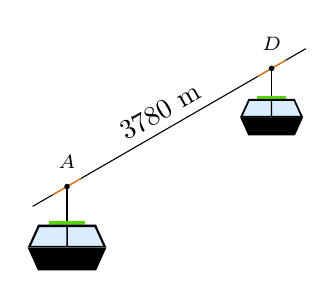
\begin{tikzpicture}[line cap=round,line join=round]
				\def\cabin{\tikz{ 
				 \draw (0,0)--(0,0.5);
				\path[fill={rgb,255:red,85; green,212; blue,0}] (-0.23,0.08)  -- (0.23,0.08) -- (0.23,0.03) -- (-0.23,0.03) -- cycle;
				\fill (0.37,-0.55) -- (-0.37,-0.55) -- (-0.5,-0.26) --  (0.5,-0.26) -- cycle;
				\path[fill={rgb,255:red,217; green,237; blue,255}] (0.37,0.03) -- (-0.37,0.03) -- (-0.5,-0.26) -- (0.5,-0.26)  -- cycle;
				 \path[fill] (0.49,-0.24) -- (0.38,0) -- (0.37,0.03) -- (-0.37,0.03) -- (-0.38,0) -- (-0.49,-0.24) -- (-0.5,-0.26) -- (0.5,-0.26) -- cycle (-0.35,0) -- (-0.01,0) -- (-0.01,-0.24) -- (-0.46,-0.24) -- cycle (0.01,-0.24) -- (0.01,0) -- (0.35,0) -- (0.46,-0.24) -- cycle;
					 }}
				\draw (-150:0.5)--(30:3.5) node[sloped,pos=0.5,above]{$3780$  m};
				\path (0,0) coordinate (A) node[anchor=north,inner sep=0pt]{\cabin} 
					(30:3) coordinate (D) node[anchor=north,inner  sep=0pt,scale=0.8]{\cabin};
				 \draw[orange] (-150:0.2)--(30:0.2)
					 (30:2.8)--(30:3.2);
				\foreach \t/\g in  {A/90,D/90}{
					\fill (\t) circle (1pt) node[shift={(\g:9pt)},font=\scriptsize]{$\t$}; 
				} 
			\end{tikzpicture}
	\end{center}
	 \shortans{840}
	 \loigiai{
		Gọi tọa độ điểm $B(550; y;  z)$.\\
		Ta  có $\overrightarrow{A B}=(540; y-3; z)$.\\
		Do đường đi của cabin cùng phương với  vectơ $\vec{u}=(2;-2; 1)$ nên ta có
		$$\dfrac{540}{2}=\dfrac{y-3}{-2}=\dfrac{z}{1} \Leftrightarrow\heva{&y-3=-540 \\ &z=270} \Leftrightarrow\heva{&y=-537 \\ &z=270} \Rightarrow B(550;-537; 270).$$ 
		Quãng đường $A B$ bằng $A B=\sqrt{540^{2}+(-537-3)^{2}+270^{2}}=810$  m.\\
		Vận tốc  của cabin bằng $v=\dfrac{A B}{3\cdot60}=4{,}5$ m/s.\\
		 Thời gian để cabin chuyển động đều từ điểm $A$ đến điểm $D$ là $\dfrac{3\,780}{4{,}5}=840$ s.
	} 
\end{bt}

% nguồn: Lop_12_Hinh_hoc_Chuong_2
\begin{bt}%[2H2V1-4]%[ma:d2dca604]
	Hình bên dưới minh họa sơ đồ một ngôi nhà trong không gian $Oxyz$, trong đó nền nhà, bốn bức tường và hai mái nhà đều là  hình chữ nhật. Tính số đo góc dốc của mái nhà, tức là số đo của góc nhị diện có cạnh là đường thẳng $FG$ hai mặt $(FGQP)$ và $(FGHE)$.
	\begin{center}
		\begin{tikzpicture}[scale=0.8,line join=round,line cap=round,>=stealth]
				 \def\r{5}
				 \def\k{3.5}
				 \path
					(0,0)  coordinate (C)
					(6,0)  coordinate (B)
					(4,-2) coordinate  (A)
					(-2,-2) coordinate (O) 
					 ($(O)+(90:\r)$) coordinate (E)
					($(A)+(90:\r)$) coordinate (F) 
					 ($(B)+(90:\r)$) coordinate (G)
					 ($(C)+(90:\r)$) coordinate (H)
					($(E)+(30:\k)$) coordinate  (P)
					($(H)+(30:\k)$)  coordinate (Q)
					 ($(O)!2!(C)$) coordinate (y)
					($(O)!1.3!(A)$) coordinate  (x)
					($(O)!1.5!(E)$) coordinate  (z);
				\draw  (O)--(A)--(B)
					(O)--(A)--(F)--(E)--cycle  (B)--(G)--(F)--(A)
					(E)--(P)--(Q)--(H)--cycle  (F)--(P)
					(G)--(Q); 
				 \draw [dashed] (H)--(G)
					 (C)--(H)
					(C)--(O) 
					 (C)--(B);
				 \draw[->,dashed](C)--(y);
				\draw[->](A)--(x)  node[left,below] {$x$};
				\draw[->](O)--(z) node[left,above]  {$z$};
				\filldraw[red] (O) circle (2pt)  node[below] {$O (0,0,1)$};
				\filldraw[red]  (B) circle (2pt) node[right] {$B (4,5,0)$};
				\filldraw[red] (Q) circle  (2pt) node[above] {$Q (2,5,4)$};
				\filldraw[red] (G) circle (2pt) node[right] {$G (4,5,3)$}; 
				\filldraw[red] (P) circle (2pt) node[right] {$P  (2,0,4)$};
				 \filldraw[red] (E) circle (2pt) node[left] {$E (0,0,3)$};
				\filldraw[fill=blue!30,opacity=0.4] (O) -- (A) --  (F) -- (E) -- cycle;
				\filldraw[fill=orange!30,opacity=0.7] (A) -- (F) --  (G) -- (B) -- cycle;
				\filldraw[fill=red!30,opacity=0.3] (F)  -- (P) -- (Q) -- (G) -- cycle;
				\filldraw[fill=red!30,opacity=0.3] (H) -- (Q) -- (P)  -- (E) -- cycle;
				\filldraw[fill=green!30,opacity=0.3]  (F) -- (P) -- (E) -- cycle;
				\foreach \i/\g  in {A/-90,C/-90,y/-90,H/90,F/-60}
				\fill  (\i) circle (1pt)+(\g:0.35) node[scale=1]{$\i$};
			\end{tikzpicture}
	\end{center}
	 \shortans{26,6}
	\loigiai{ 
		Để tính góc của  mái nhà, ta tính số đo của góc nhị diện có cạnh là đường thẳng $FG$, hai mặt lần lượt là $(FGQP)$ và $(FGHE)$.\\
		Do mặt mặt phẳng $(Oxy)$ vuông góc với hai mặt phẳng $(FGPQ)$ và $(FGHE)$.\\ 
		Ta có  $\heva{&(Oxy)\perp (FGQP)\\&(Oxy)\perp (FGHE)\\&FP=(Oxy)\cap (FGQP)\\&FE=(Oxy)\cap (FGEH)}\Rightarrow \widehat {PFE}$ là góc phẳng nhị diện cần tìm.\\
		Tứ giác $(OAFE)$ là hình chữ nhật nên  $x_F=x_A=4$, $z_F=z_E=3$.\\
		Do $F$ nằm trên mặt phẳng $(Oxz)$ nên  tọa độ điểm $F(4;0;3)$.\\
		Ta có  $\overrightarrow{FP}=(-2;0;1)$, $\overrightarrow{FE}=(-4;0;0)$, suy ra
		\begin{eqnarray*}
			\cos  \widehat{PFE}&=&\cos \big(\overrightarrow{FP};\overrightarrow{FE}\big)\\
			&=&\dfrac{\overrightarrow{FP}\cdot  \overrightarrow{FE}}{FP\cdot FE}\\
			&=&\dfrac{(-2)\cdot(-4)+0\cdot0+1\cdot0}{\sqrt{(-2)^2+0^2+1^2}\sqrt{(-4)^2+0^2+0^2}}\\ 
			 &=&\dfrac{2\sqrt{5}}{5}.
		\end{eqnarray*}
		Suy ra $\widehat{PFE}=26{,}6^\circ$. Vậy góc dốc mái nhà  khoảng $26{,}6^\circ$.
	} 
\end{bt}

% nguồn: Lop_12_Hinh_hoc_Chuong_2
\begin{bt}%[2H2V1-4]%[ma:d91c0563]
	\immini[thm]{Một chiếc đèn trang trí (gồm các bóng đèn gắn vào một giá hình tròn) như hình bên dưới. Đèn được treo song song với mặt phẳng nằm ngang bởi ba sợi dây không dãn xuất phát  từ điểm $O$ trên trần nhà và lần lượt buộc vào ba điểm $A$, $B$, $C$ trên giá sao cho tam giác $ABC$ đều. Độ dài của ba đoạn dây $OA$, $OB$, $OC$ đều bằng $L$, trọng lượng của chiếc đèn là $27$ N, bán kính của giá hình tròn là $0{,}5$ m.
	Biết rằng mỗi sợi dây đó được thiết kế để chịu được lực căng tối đa là $12$ N. Hỏi chiều dài tối thiểu của mỗi sợi dây là bao nhiêu mét? (kết quả làm tròn đến hàng phần trăm).}{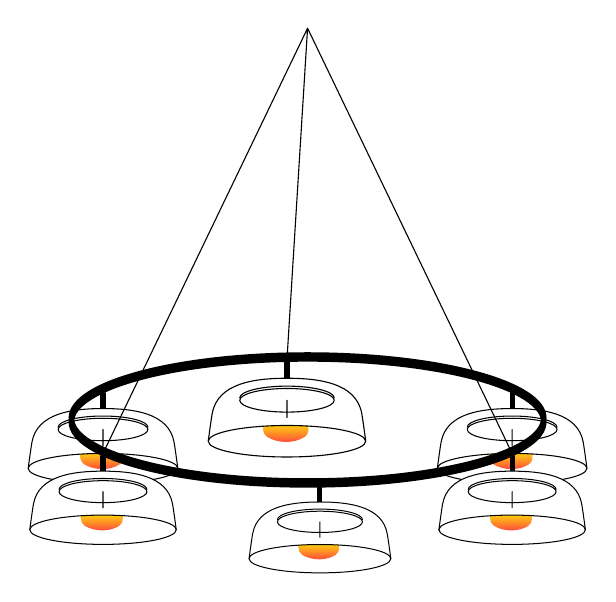
\begin{tikzpicture}[line cap=round,line join=round]
		 \def\longden{\tikz{
		\draw[line  width=2pt] (0,-0.2)--(0,0);
		\draw[fill=white] (-1,-1)..  controls +(0:0) and +(-100:0.1).. (-0.95,-0.65).. controls +(80:0.4) and +(180:0.4).. (0,-0.2).. controls +(0:0.4) and +(100:0.4).. (0.95,-0.65).. controls +(-80:0.1) and +(0:0).. (1,-1);
		\begin{scope}
			\clip  (0,-1) ellipse (1 and 0.2);
			\path[bottom color=red!75,top  color=yellow,rounded corners=2pt]
				(-0.29,-0.71) -- (-0.31,-0.91).. controls (-0.11,-1.03) and  (0.09,-1.03)..
				 (0.28,-0.91) -- (0.26,-0.73);
		\end{scope}
		\draw (0.6,-0.45) arc (0:180:0.6  and 0.15);
		\draw (0,-0.48) ellipse (0.6  and 0.15)
			 (0,-0.48)--+(0,-0.22)
			(0,-1) ellipse (1 and  0.2);
			}} 
		\path (95:3 and 0.8)  node[anchor=north,inner sep=0pt]{\longden};
		\path (30:3 and 0.8) node[anchor=north,inner sep=0pt,scale=0.95]{\longden} 
			(150:3  and 0.8) node[anchor=north,inner sep=0pt,scale=0.95]{\longden};
		\path  (-30:3 and 0.8) node[anchor=north,inner sep=0pt,scale=0.93]{\longden}
			(-150:3 and 0.8) node[anchor=north,inner sep=0pt,scale=0.93]{\longden}; 
		\path  (273:3 and 0.8) node[anchor=north,inner sep=0pt,scale=0.9]{\longden};
		 \draw (0,5)--(95:3 and 0.8)
			 (-30:3 and 0.8)--(0,5)--(210:3 and 0.8);
		\draw[line width=0.07cm] (0,0) ellipse  (3 and 0.8)
			(0,0.05) ellipse (3 and  0.8);
	\end{tikzpicture}
	 }
	 \shortans{0,76}
	 \loigiai{
	\immini{Gọi $G$ là trọng tâm tam giác $ABC$.  Vì tam giác $ABC$ đều nên $G$ là tâm đường tròn ngoại tiếp tam giác $ABC$. \\
		Do đó, $GA = GB = GC = 0{,}5$ m. Gọi $F$ là độ lớn của các lực căng $\overrightarrow{F}_1$, $\overrightarrow{F}_2$, $\overrightarrow{F}_3$ trên  mỗi sợi dây. Khi đó, $F = F(L)$ là một hàm số với biến số là $L$.\\
		Ta có $OA = OB = OC = L$ nên $\heva{&OG \perp (ABC) \\ &\left|\vec{OA}\right| = \left|\vec{OB}\right| =  \left|\vec{OC}\right| = L.}$\\
		Do đó, $\left|\vec{F_1}\right| = \left|\vec{F_2}\right| = \left|\vec{F_3}\right|$.}{ 
		\begin{tikzpicture}[declare function={r=3;},scale=.8,font=\footnotesize]
				\path (160:{r} and  {r*0.35}) coordinate (A)
					 (260:{r} and {r*0.5}) coordinate (C)
					 (20:{r} and {r*0.35}) coordinate (B)
					 (90:{r*1.25}) coordinate (O);
				 \draw[dash pattern=on 2pt off 2 pt] (A)--(B);
				\draw (A)--(C)--(B)--(O)--cycle  (O)--(C);
				 \path
					($(O)!1/3!(A)$)  coordinate (a)
					 ($(O)!1/3!(B)$) coordinate (b)
					($(O)!1/3!(C)$)  coordinate (c)
					($(B)!.5!(C)$) coordinate (M) 
					($(A)!2/3!(M)$) coordinate (G) 
					 ($(O)!3/2!(G)$) coordinate (g);
				\draw[->,red](O)--(a) node[left]{$\overrightarrow{F}_1$}; 
				\draw[->,red](O)--(b) node[right]{$\overrightarrow{F}_2$}; 
				\draw[->,red] (O)--(c) node[left]{$\overrightarrow{F}_3$}; 
				\draw[->,red]  (G)--(g) node[right]{$\overrightarrow{P}$};
				 \draw[dashed](O)--(G)--(A)
					(C)--(G)--(B); 
				\foreach  \x/\g in {A/-90,B/0,C/-90,O/0,G/60}\fill (\x) circle (1pt)+(\g:.3) node{$\x$};
			\end{tikzpicture}
		} 
		 \noindent
		Vì vậy tồn tại hằng số $c \neq 0$ sao cho $\vec{F_1} = c\vec{OA}$, $\vec{F_2} =  c\vec{OB}$, $\vec{F_3} = c\vec{OC}$.\\
		Suy ra $\vec{F_1} + \vec{F_2} + \vec{F_3} = c\left(\vec{OA} + \vec{OB} +  \vec{OC}\right) = 3c\vec{OG}$.\\
		Mặt khác, ta lại có $\vec{F_1} + \vec{F_2} + \vec{F_3} =  \vec{P}$ với $\vec{P}$ là trọng lực tác dụng lên chiếc đèn.\\
		Mà trọng lực tác dụng lên chiếc đèn là $27$ (N) nên $\left|\vec{P}\right| = 27 \Rightarrow 3c\left|\vec{OG}\right| = 27 \Rightarrow c  = \dfrac{9}{OG}$.\\
		Tam giác $AOG$ vuông tại $G$ (do $OG \perp (ABC)$) nên ta suy ra $OG = \sqrt{OA^2 - GA^2} = \sqrt{L^2 - 0{,}5^2}$ (m) với $L >  0{,}5$.\\
		Do đó, $OG = \sqrt{L^2 -  0{,}5^2} \Rightarrow c = \dfrac{9}{\sqrt{L^2 - 0{,}5^2}}$.\\
		Khi đó, $\left|\vec{F}\right| = \left|\vec{F_1}\right| = c\left|\vec{OA}\right| = \dfrac{9L}{\sqrt{L^2 - 0{,}5^2}}$ (với $L  > 0{,}5$).\\
		Ta có lực căng tối đa của  mỗi sợi dây là $12$ (N).\\
		Suy ra \begin{eqnarray*}
		&& F(L) \le 12 \Leftrightarrow \dfrac{9L}{\sqrt{L^2 -  0{,}5^2}} \le 12 \\
		&\Leftrightarrow& 3L \le 4\sqrt{L^2 - 0{,}5^2}\\  &\Leftrightarrow& 9L^2 \le 16L^2 - 4 \\
		&\Leftrightarrow&  7L^2 \ge 4\\
		&\Rightarrow&  L \ge \dfrac{2\sqrt{7}}{7}.
	\end{eqnarray*}
Vậy chiều dài tối thiểu  của mỗi sợi dây là $\dfrac{2\sqrt{7}}{7} \approx 0{,}76$ (m).}
\end{bt}

% nguồn: Lop_12_Hinh_hoc_Chuong_2
\begin{bt}%[2H2V1-4]%[ma:ed733884]
	Để chuẩn bị cho một buổi triển lãm quốc tế, các trang sức có giá trị lớn được đặt bảo mật trong các khối chóp tứ giác đều $S.A B C D$ và đặt lên phía trên một trụ hình hộp chữ nhật $A B C D . A^{\prime} B^{\prime} C^{\prime} D^{\prime}$ có đáy là hình vuông (như hình vẽ). Chọn hệ trục tọa độ Oxyz (đơn vị trên mỗi trục là mét) sao cho $A^{\prime}(0; 0; 0), A(0; 0; 1), B(0;  0{,}5; 1)$. Biết rằng, ban tổ chức sự kiện dự định dùng các tấm kính cường lực
	hình tam giác cân có cạnh bên là $60$ cm để lắp ráp thành khối chóp nói trên. Khi  đó, tọa độ điểm $S$ là $(a; b; c)$. Tính giá trị của $a+b+c$. Làm tròn kết quả đến hàng phần trăm.
	\begin{center}
		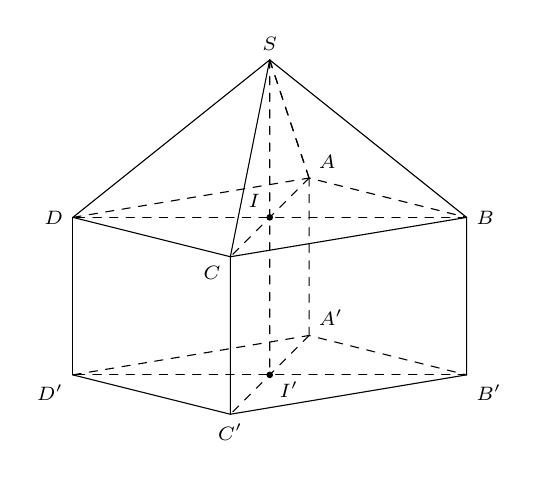
\begin{tikzpicture}[scale=1,font=\scriptsize,line join=round,line cap=round,>=stealth]
				 \draw[dashed] (0,0)--(3,0.5)--(5,0)
					 (3,0.5)--(3,2.5)
					(0,2)--(3,2.5)--(5,2) 
					 (2.5,4)--(3,2.5);
				\draw (5,0)--(5,2)--(2,1.5)--(0,2) 
					(2.5,4)--(0,2) 
					(2,-0.5)--(2,1.5) 
					(2.5,4)--(2,1.5); 
				 \draw (0,0)--(2,-0.5);
				\draw (0,2)--(0,0); 
				 \draw (2,-0.5)--(5,0);
				\draw  (2.5,4)--(5,2);
				 \draw[dashed] (2.5,4)--(3,2.5);
				\node[below left] at (0,0)  {$D'$};
				\node[below] at (2,-0.5)  {$C'$};
				\node[below  right] at (5,0) {$B'$};
				\node[left] at (0,2) {$D$}; 
				\node[above right] at (3,0.5) {$A'$}; 
				\node[right] at (5,2) {$B$}; 
				 \node[below left] at (2,1.5) {$C$};
				\node[above  right] at (3,2.5) {$A$};
				\node[above] at (2.5,4) {$S$}; 
				 \coordinate (A) at (3,2.5);
				\coordinate (B)  at (5,2);
				 \coordinate (C) at (2,1.5);
				 \coordinate (D) at (0,2);
				\coordinate (A') at (3,0.5); 
				\coordinate  (B') at (5,0);
				\coordinate (C')  at (2,-0.5);
				\coordinate (D') at (0,0); 
				\coordinate  (S) at (2.5,4);
				 \coordinate (I) at (intersection cs: first line={(A)--(C)},second line={(B)--(D)});
				\fill  (I) circle (1.2pt) node[above left] {$I$};
				\coordinate (I') at (intersection cs: first line={(A')--(C')},second line={(B')--(D')}); 
				\fill (I') circle (1.2pt) node[below  right,yshift=1pt] {$I'$};
				 \draw[dashed] (A)--(C);
				\draw[dashed] (B)--(D); 
				 \draw[dashed] (A')--(C');
				 \draw[dashed] (B')--(D');
				 \draw[dashed] (S)--(I');
			\end{tikzpicture}
	\end{center}
	 \shortans{1,98}
	 \loigiai{
		Đổi $60$ cm $=0{,}6$ m.\\ 
		 Ta có $S A=0{,}6$ m.\\
		$A^{\prime}(0; 0; 0), A(0; 0; 1), B(0; 0{,}5; 1) \Rightarrow A B=\dfrac{1}{2}, A A^{\prime}=1$.\\ 
		Gọi $I=A C  \cap B D, I^{\prime}=A^{\prime} C^{\prime} \cap B^{\prime} D^{\prime}$.\\
		Vì $S . A B C D$ là khối chóp tứ giác đều nên $A B C  D$ là hình vuông và $S I \perp(A B C D)$.\\
		Vì $A B C D . A^{\prime} B^{\prime} C^{\prime} D^{\prime}$ là hình hộp chữ nhật nên $(A B C  D) \parallel \left(A^{\prime} B^{\prime} C^{\prime} D^{\prime}\right), I I^{\prime} \perp\left(A^{\prime} B^{\prime} C^{\prime} D^{\prime}\right)$.\\
		Do đó $S I \perp\left(A^{\prime} B^{\prime} C^{\prime} D^{\prime}\right)$.  \\
		Suy ra $S,  I, I^{\prime}$ thẳng hàng.\\
		Vì vậy $S I^{\prime} \perp\left(A^{\prime} B^{\prime} C^{\prime} D^{\prime}\right)$.\\ 
		Xét tam giác vuông $A B  C$ có $A C=\sqrt{A B^{2}+B C^{2}}=\sqrt{\left(\dfrac{1}{2}\right)^{2}+\left(\dfrac{1}{2}\right)^{2}}=\dfrac{\sqrt{2}}{2} \Rightarrow A I=\dfrac{\sqrt{2}}{4}$.\\
		Xét tam giác vuông  $S I A$ có $S I=\sqrt{S A^{2}-A I^{2}}=\sqrt{0{,}6^{2}-\left(\dfrac{\sqrt{2}}{4}\right)^{2}}=\dfrac{\sqrt{94}}{20}$.\\
		Gọi $I^{\prime}$  là trung điểm của $A^{\prime} C^{\prime} \Rightarrow I I^{\prime}=A A^{\prime}=1 \Rightarrow S I^{\prime}=I I^{\prime}+S I=1+\dfrac{\sqrt{94}}{20}=\dfrac{20+\sqrt{94}}{20}$.\\
		Ta có $A A^{\prime} B^{\prime} B$ là hình chữ nhật và $A^{\prime}(0; 0; 0), A(0; 0; 1), B(0; 0{,}5; 1) \Rightarrow B^{\prime}(0; 0{,}5; 0)  \in O y$.\\
		Mà $A^{\prime}(0; 0; 0) \equiv O, A(0; 0; 1) \in O z \Rightarrow D^{\prime} \in Ox$.\\ 
		Vì $A B C D$ là hình vuông nên $A^{\prime} B^{\prime} C^{\prime} D^{\prime}$ là hình  vuông cạnh $\dfrac{1}{2}$.\\
		Suy  ra $A^{\prime} D^{\prime}=\dfrac{1}{2} \Rightarrow D^{\prime}(0{,}5; 0; 0) \Rightarrow I^{\prime}(0{,}25; 0{,}25; 0)$.\\
		Vì $I^{\prime}(0{,}25; 0{,}25; 0)$ là hình chiếu của $S$ trên mặt phẳng  $Oxy$ và $S I^{\prime}=\dfrac{20+\sqrt{94}}{20}$ nên $$ S\left(0{,}25; 0{,}25; \dfrac{20+\sqrt{94}}{20}\right).$$
	Do đó $ a+b+c=0{,}25+0{,}25+\dfrac{20+\sqrt{94}}{20}  \approx 1{,}98$.}
\end{bt}

% nguồn: Lop_12_Hinh_hoc_Chuong_2
\begin{bt}%[2H2V1-4]%[ma:69264c15]
	Một chiếc xe đang  kéo căng sợi dây cáp $A B$ trong công trường xây dựng, trên đó đã thiết lập hệ toạ độ $Oxyz$ như hình vẽ dưới với độ dài đơn vị trên các trục tọa độ bằng $1$ m. Biết $\overrightarrow{A B}=(x; y; z)$. Tính $x+2 y-z$ (làm tròn đến hàng phần mười).
	\begin{center}
		\begin{tikzpicture}[line join = round,line cap=round,>=stealth,font=\footnotesize,scale=0.7]
				\path (0,0) coordinate  (O)
					(5,0) coordinate (H) 
					(-2,-2) coordinate (K) 
					($(K)+(H)-(O)$) coordinate  (B)
					($(O)+(0,3.6)$)  coordinate (A);
				 \foreach \x/\y in{K/x,H/y,A/z}
				\draw[->,line  width=1pt,scale=1.5] (O)--(\x)--($(O)!1.4!(\x)$) node[right]{$\y$};
				 \draw[pattern=crosshatch] (-0.2,0) rectangle (0.3,4)
					 (-2.5,3.6) rectangle (0.3,4);
				\draw[pattern=crosshatch,rotate=-50,xshift=-3cm,yshift=2.4cm] 
					(-0.2,0) rectangle (0.3,1.5); 
				 \draw[cyan,line width=4pt] (O)--(A);
				\foreach \x/\goc/\t in {A/0/A,K/180/K,H/90/H,B/70/B,O/-90/O} 
				\draw[fill=white] (\x) circle (1pt) node[shift={(\goc:7pt)},font=\scriptsize]{$\t$}; 
				\draw[dashed] (O)--($(O)-(1,0)$); 
				\draw[<->,line width=2pt]  ($(O)-(1,0)$)--($(A)-(1,0)$)
					node[pos=0.5,left,font=\footnotesize]{$10$ m}; 
				\draw[line width=1pt]  (O)--(B)
					 node[pos=0.45,below,rotate=-30,font=\footnotesize]{$15$ m};
				\draw (K)--(B)--(H) 
					(B)--(O); 
				\draw  pic[draw,angle radius=6mm] {angle = B--O--H};
				\draw ($(O)+(1.2,-0.25)$)  node{$30^\circ$};
				\draw[->,line width=2pt]  (A)--(B);
				\draw (B)  node[xshift=0.5cm,yshift=-0.5cm]{
			\begin{tikzpicture}[line join = round,line cap=round,>=stealth,font=\footnotesize,scale=0.4]
					\draw[rotate=-65,scale=1,line width=5pt,xshift=1.8cm,yshift=2.4cm] (0.7,-1.5) ellipse  (0.4cm and 0.3cm);
					 \fill[green!80] (0,0)--(0,-1)--(1,-2)--(2,-2)--(2,-1)--(1,0)--cycle;
					 \draw (0,0)--(0,-1)--(1,-2)--(2,-2)--(2,-1)--(1,0)--cycle;
					\draw[rotate=-65,scale=1,line width=5pt] (1,-0.4) ellipse (0.4cm and 0.3cm); 
					\draw[rotate=-65,scale=1,,line width=5pt,xshift=1.4cm,yshift=1.5cm] (0.7,-1.5) ellipse (0.4cm  and 0.3cm);
				\end{tikzpicture}
		}; 
	\end{tikzpicture}
\end{center}
 \shortans{43,5}
\loigiai{ 
	Vì $\overrightarrow{O A}$ cùng hướng với $\vec{k}$ và $O A=10$ nên $\overrightarrow{O A}=10 \vec{k}$.\\ 
	Xét $\triangle O B H$ vuông tại $H$, có $B H=O B \cdot \sin 30^{\circ}=15 \cdot  \dfrac{1}{2}=7{,}5$ m.\\
	 $O H=O B \cdot \cos 30^{\circ}=15 \cdot\dfrac{\sqrt{3}}{2}=\dfrac{15 \sqrt{3}}{2}$ m.\\
	Vì $\overrightarrow{O H}$ cùng  hướng với $\vec{j}$ nên $\overrightarrow{O H}=\dfrac{15 \sqrt{3}}{2} \vec{j}$.\\
	Vì $\overrightarrow{A B}=\overrightarrow{O B}-\overrightarrow{O A}=\overrightarrow{O  H}+\overrightarrow{O K}-\overrightarrow{O A}=7,5 \vec{i}+\dfrac{15 \sqrt{3}}{2} \vec{j}-10 \vec{k}$.\\
	Do  đó $\overrightarrow{A B}=\left(7,5; \dfrac{15 \sqrt{3}}{2};-10\right)$.\\
Vậy $x+2 y-z=7{,}5+2 \cdot \dfrac{15 \sqrt{3}}{2}+10  \approx 43{,}5$ m.}
\end{bt}

% nguồn: Lop_12_Hinh_hoc_Chuong_2
\begin{bt}%[2H2V1-4]%[ma:b682464d]
	Trong không gian, cho tứ diện  $ABCD$ có các điểm $M$, $N$, $P$ lần lượt thuộc các cạnh $BC$, $BD$ và $AC$ sao cho $\overrightarrow{BC}=4\overrightarrow{BM}$, $ \overrightarrow{AC}=3\overrightarrow{AP}$, $ \overrightarrow{BD}=2\overrightarrow{BN}$. Mặt phẳng $\left(MNP\right)$ cắt đường thẳng $AD$ tại điểm $Q$.
	Tính tỉ  số $\dfrac{AQ}{AD}$.
	 \shortans{0,6}
	\loigiai{ 
		\begin{center}
			\begin{tikzpicture}[scale=1.5,line join=round]
					\coordinate[label=above:  $A$] (A) at (-0.2,2.2);
					\coordinate[label=left: $B$] (B) at (-1,0); 
					 \coordinate[label=right: $D$] (D) at (3,0);
					\coordinate[label=below: $C$] (C)  at (1,-0.8);
					 \coordinate[label=above: $N$] (N) at ($(B)!0.5!(D)$);
					 \coordinate[label=below: $M$] (M) at ($(B)!0.25!(C)$);
					\coordinate[label=left: $P$] (P) at ($(A)!0.333!(C)$); 
					\coordinate[label=above: $Q$] (Q) at  ($(A)!0.6!(D)$);
					\coordinate[label=right:$R$]  (R) at (4,0.4);
					\draw (A) -- (B) --  (C) -- (D) -- cycle (A) -- (C);
					\draw  (A) -- (D)
						(M)  -- (P)
						 (P)--(R);
					\draw[dashed] (B)  -- (D)
						(P) --  (N);
					\draw[dashed] (M) -- (R); 
					\foreach \pt in {A,B,C,D,R,M,N,Q,P} 
					\fill (\pt)  circle (1.5pt);
				\end{tikzpicture}
		\end{center}
		Đặt  $\overrightarrow{AB}=\overrightarrow{a}$, $\overrightarrow{AC}=\overrightarrow{b}$, $\overrightarrow{AD}=\overrightarrow{c}$, $\overrightarrow{AQ}=k \overrightarrow{AD}=k \overrightarrow{c}$.\\
		Theo  đề bài, ta có $\overrightarrow{AM}=\dfrac{3}{4}\overrightarrow{a}+\dfrac{1}{4}\overrightarrow{b}$; $ \overrightarrow{AN}=\dfrac{1}{2}(\overrightarrow{a}+\overrightarrow{c})$; $\overrightarrow{AP}=\dfrac{1}{3}\overrightarrow{b}$.\\
		Ta có  $\heva{&\overrightarrow{MN}=\overrightarrow{AN}-\overrightarrow{AM}=-\dfrac{1}{4}\overrightarrow{a}-\dfrac{1}{4}\overrightarrow{b}+\dfrac{1}{2}\overrightarrow{c}\\
		&\overrightarrow{MP}=\overrightarrow{AP} - \overrightarrow{AM}=-\dfrac{3}{4}\overrightarrow{a}+\dfrac{1}{12}\overrightarrow{b}\\ 
		&\overrightarrow{MQ}=\overrightarrow{AQ} -  \overrightarrow{AM}=-\dfrac{3}{4}\overrightarrow{a}-\dfrac{1}{4}\overrightarrow{b}+k \overrightarrow{c}.}$\\
		Vì $M$, $N$, $P$, $Q$ đồng phẳng nên  $x\overrightarrow{MN}+y\overrightarrow{MP}=\overrightarrow{MQ} \Leftrightarrow
		\heva{ 
		 &0{,}25x+0{,}75y=0{,}75 \\
		&0{,}25x-\dfrac{1}{12}y=0{,}25  \\
		&0{,}5x=k} 
		\Leftrightarrow 
		\heva{ 
		&x=\dfrac{3}{5} \\ 
		&y=\dfrac{3}{5} \\ 
		&k=\dfrac{3}{5} 
		.} 
		$\\ 
	Vậy $\dfrac{AQ}{AD}=\dfrac{3}{5}=0{,}6$.} 
\end{bt}

% nguồn: Lop_12_Hinh_hoc_Chuong_2
\begin{bt}%[2H2V1-4]%[ma:e20ea898]
	\immini[thm]{Có ba lực cùng tác động vào một cái bàn như hình vẽ. Trong đó hai lực $\vec{F}_1$, $\vec{F}_2$ có giá nằm trên mặt phẳng chứa mặt bàn, tạo với nhau một góc $110^\circ$ và có độ lớn lần lượt là $9$ (N) và $4$ (N), lực $\vec{F}_3$ vuông góc với mặt bàn và có độ lớn $7$ (N). Độ lớn hợp lực của ba lực  trên là $a$ (N), tìm giá trị của $a$. (kết quả quy tròn về số nguyên).
	 \shortans{11}
	}{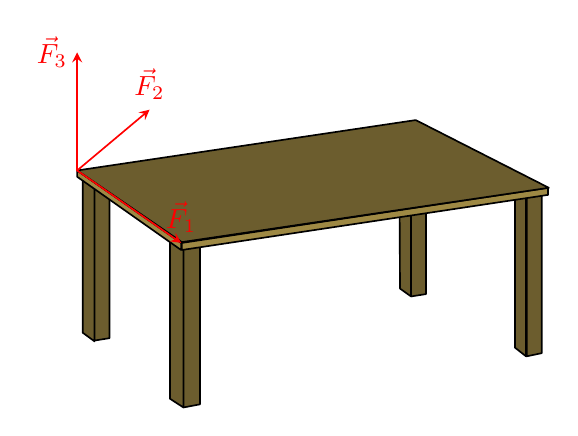
\begin{tikzpicture}[line cap=round,line join=round,semithick,>=stealth]
		 \definecolor{c6c5d2e}{RGB}{108,93,46}
		 \definecolor{c9e8944}{RGB}{158,137,68}
		\path[draw,fill=c6c5d2e] (0.23,-1.87) -- (0.23,-3.96) --  (0.42,-3.93) -- (0.42,-1.84) -- cycle
			(0.08,-1.82) -- (0.08,-3.86) --  (0.23,-3.97) -- (0.23,-1.86) -- cycle
			(5.72,-2.07) -- (5.72,-4.16) -- (5.91,-4.12)  -- (5.91,-2.04) -- cycle
			 (5.57,-2.01) -- (5.57,-4.05) -- (5.71,-4.16) -- (5.71,-2.05) -- cycle
			(4.25,-1.36)  -- (4.25,-3.4) -- (4.44,-3.37) -- (4.44,-1.33) -- (4.25,-1.36) -- cycle
			(4.1,-1.3) -- (4.11,-3.3) -- (4.25,-3.4) -- (4.25,-1.34) --  cycle
			(1.36,-2.63) -- (1.36,-4.81) --  (1.57,-4.77) -- (1.57,-2.6) -- cycle
			(1.19,-2.57)  -- (1.19,-4.7) -- (1.36,-4.81) -- (1.36,-2.61) -- cycle;
		\path[draw,fill=c9e8944] 
			(1.33,-2.81)  -- (0.01,-1.88) -- (0.01,-1.8) -- (1.33,-2.72) -- cycle
			(1.34,-2.72) -- (1.34,-2.81) --  (5.99,-2.11) -- (5.99,-2.02) --cycle;
		\path[draw,fill=c6c5d2e] (0.01,-1.8) -- (1.34,-2.71) -- (6,-2.02) -- (4.31,-1.16) -- (0.01,-1.8) --  cycle;
		 \draw[red,->](0.01,-1.8) coordinate (O) -- (1.33,-2.72) node[above]{$\vec{F}_1$};
		\draw[red,->] (O) -- +(90:1.5) node[left]{$\vec{F}_3$}; 
		\draw[red,->] (O) -- +(40:1.2)  node[above]{$\vec{F}_2$};
	\end{tikzpicture}
	 }
	 \shortans{11}
	 \loigiai{
		Ta có\begin{eqnarray*}
		 \left|\vec{F}_{12}\right| = \left|\vec{F}_1 + \vec{F}_2\right| &=& \sqrt{\left|\vec{F}_1\right|^2 + \left|\vec{F}_2\right|^2 + 2\left|\vec{F}_1\right|\left|\vec{F}_2\right|\cos\left(\vec{F}_1, \vec{F}_2\right)}\\
		&=& \sqrt{9^2 + 4^2 + 2 \cdot  9 \cdot 4 \cdot \cos 110^\circ} \approx 8{,}5.
	\end{eqnarray*}
	$\vec{F}  = \vec{F}_1 + \vec{F}_2 + \vec{F}_3 = \vec{F}_{12} + \vec{F}_3 \Rightarrow \left|\vec{F}\right| = \sqrt{\left|\vec{F}_{12}\right|^2 + \left|\vec{F}_3\right|^2} = \sqrt{(8{,}5)^2 + 7^2} \approx 11$ (N).\\
Vậy $a$ xấp xỉ $11$.} 
\end{bt}

% nguồn: Lop_12_Hinh_hoc_Chuong_2
\begin{bt}%[2H2V1-4]%[ma:eabd344b]
	Trong không gian, cho hình hộp $ABCD.A'B'C'D'$. Biết $\overrightarrow{MA'}=k\cdot\overrightarrow{MC}$, $\overrightarrow{NC'}=l\cdot \overrightarrow{ND}$. Khi $MN$ song song với $BD'$ thì $k+l$ có  giá trị là bao nhiêu?
	\shortans{-4} 
	\loigiai{ 
		\begin{center}
			\begin{tikzpicture}[scale=0.6,font=\footnotesize,line join=round,line cap=round]
					 \def\h{4}
					\foreach  \x\y\t in {0/0/A,-1/-1.1/B,2.6/-1.1/C}
					\coordinate  (\t) at (\x,\y);
					\coordinate (D)  at ($(A)+(C)-(B)$);
					\coordinate (A') at ($(A)+(0,3.2)$); 
					\coordinate (B')  at ($(B)+(0,3.2)$);
					\coordinate (C') at ($(C)+(0,3.2)$); 
					\coordinate (D') at ($(D)+(0,3.2)$); 
					\draw (B')--(A')--(D')--(C')--(B')--(B)--(C)--(D)--(D') 
						 (C')--(C);
					 \draw[dashed](B)--(A)--(D)
						 (A)--(A');
					 \foreach \t/\g in {A/170,B/-150,C/-70,D/0,A'/100,B'/170,C'/-20,D'/50}
					\draw  (\t) circle (1pt)
						node[shift={(\g:7pt)}]{$\t$}; 
				\end{tikzpicture}
		\end{center}
		Đặt $\overrightarrow{AB}=\overrightarrow{a}$ , $\overrightarrow{AD}=\overrightarrow{b}$  , $\overrightarrow{AA'}=\overrightarrow{c}$.\\
		Ta có $\overrightarrow{MA'}=k\cdot\overrightarrow{MC} \Leftrightarrow \overrightarrow{AA'} -  \overrightarrow{AM}=k\left(\overrightarrow{AC} - \overrightarrow{AM}\right) \Leftrightarrow \overrightarrow{AM}=\dfrac{-k\left(\overrightarrow{a}+\overrightarrow{b}\right)+\overrightarrow{c}}{1-k}$.\\
		Mặt khác  $\overrightarrow{NC'}=l\cdot\overrightarrow{ND} \Leftrightarrow \overrightarrow{AN}=\dfrac{\overrightarrow{a}+\overrightarrow{b}+\overrightarrow{c}-l\overrightarrow{b}}{1-l}$.\\
		Suy ra  $\overrightarrow{MN}=\overrightarrow{AM}-\overrightarrow{AN}=\left(-\dfrac{k}{1-k}-\dfrac{1}{1-l}\right)\overrightarrow{a}+\left(-\dfrac{k}{1-k}-1\right)\overrightarrow{b}+\left(\dfrac{1}{1-k}-\dfrac{1}{1-l}\right)\overrightarrow{c}$.\\
		Hơn nữa $\overrightarrow{BD'}=\overrightarrow{AD'} - \overrightarrow{AB}=-\overrightarrow{a}+\overrightarrow{b}+\overrightarrow{c}$.\\ 
		Vì $MN\parallel BD'$ nên $\overrightarrow{MN} \parallel \overrightarrow{BD'}  \Leftrightarrow \dfrac{3k+1}{1-k}=-2 \Leftrightarrow k=-3 \Rightarrow l=-1$.\\
	Vậy  $k+l=-4$.}
\end{bt}

% nguồn: Lop_12_Hinh_hoc_Chuong_2
\begin{bt}%[2H2V1-4]%[ma:eef5618b]
	Người ta treo một chiếc đèn trang trí có trọng lượng $200$ N lên trên trần nhà bằng ba sợi dây không giãn, bằng nhau tại ba điểm $A$, $B$, $C$ tạo thành tam giác đều. Mỗi sợi dây tạo với mặt phẳng trần nhà một góc $30^{\circ}$ và được giữ ở trạng thái cân bằng. Tính lực căng của mỗi sợi  dây (kết quả làm tròn đến hàng đơn vị).
	 \shortans{133}
	\loigiai{ 
		\begin{center}
			\begin{tikzpicture}[>=stealth,line join=round,line cap=round,font=\footnotesize,scale=1]
					\coordinate (A) at  (0,0);
					\coordinate (B)  at (5,2);
					\coordinate (C)  at (7,0);
					\coordinate  (M) at ($(B)!1/2!(C)$);
					\coordinate (G) at  ($(A)!2/3!(M)$);
					\coordinate  (S) at ($(G)+(0,-3)$);
					\coordinate (P)  at ($(S)!1/2!(A)$);
					\coordinate  (Q) at ($(S)!2/5!(B)$);
					\coordinate (R) at  ($(S)!1/2!(C)$);
					\coordinate (H) at  ($(S)+(0,-3)$);
					\draw  (A)--(B)--(C)--(A)--(M)
						 (G)--(B)
						 (G)--(C);
					\draw  [->] (S)--(A);
					 \draw [->] (S)--(C);
					\draw [->] (S)--(H) node  [below]{$\overrightarrow{P}$};
					\draw [dashed,->] (S)--(M); 
					 \draw [dashed,->] (S)--(G);
					\draw  [dashed,->] (S)--(B);
					\draw [->,line width=1.3,color=red] (S)--(P)  node [left]{$\overrightarrow{F}_1$};
					\draw [->,line width=1.3,color=red] (S)--(Q) node [right]{$\overrightarrow{F}_2$}; 
					 \draw [->,line width=1.3,color=red] (S)--(R) node [right]{$\overrightarrow{F}_3$};
					\foreach \x/\g in {A/90,B/90,C/0,M/30,G/145,S/-45}\fill  (\x)+(\g:3mm) node{$ \x $};
				\end{tikzpicture}
		\end{center}
		Giả sử $\alpha$ là góc hợp bởi sợi dây và mặt phẳng trần nhà. Ta  có $\alpha=30^{\circ}$.\\
		Xét tứ diện $S.ABC$ có các cạnh $SA, SB,  SC$ biểu diễn độ lớn lực căng dây và $SP$ biểu diễn độ lớn của trọng lực tác dụng lên vật $S$.\\
		Với $G$ là trọng tâm của tam giác đều $ABC$, ta có \begin{center}
		$\left|\overrightarrow{F}_1\right|=SA; \left|\overrightarrow{F}_2\right|=SB; \left|\overrightarrow{F}_3\right|=SC,  \left|\overrightarrow{P}\right|=SG$ và $3\overrightarrow{SG}+\overrightarrow{SP}=\vec{0}$.
	\end{center}
	Do hệ cân bằng nên ta có \[\overrightarrow{SA}+\overrightarrow{SB}+\overrightarrow{SC}+\overrightarrow{P}=\vec{0}.\] 
	Theo phương thẳng  đứng, ta có \[F_1\sin{\alpha}+F_2\sin{\alpha}+F_3\sin{\alpha}=P\Leftrightarrow 3F_1\sin{\alpha}=P\Leftrightarrow F_1=\dfrac{P}{3\sin{\alpha}}=\dfrac{200}{3\sin{30^{\circ}}}=\dfrac{400}{3}\approx 133 (\mathrm{N}).\]
} 
\end{bt}

% nguồn: Lop_12_Hinh_hoc_Chuong_2
\begin{bt}%[2H2V1-4]%[ma:f23afbe4]
	Hình sau đây minh họa sơ đồ một ngôi nhà trong hệ trục tọa độ $Oxy$, trong đó nền nhà, bốn bức tường và hai mái nhà đều là hình chữ nhật. Biết $F(a;b;c)$. Giá  trị của tổng $a+b+c$ bằng bao nhiêu?
	\begin{center}
		\begin{tikzpicture}[scale=0.8,line join=round,line cap=round,>=stealth]
				 \def\r{5}
				\def\k{3.5} 
				 \path
					(0,0) coordinate (C) 
					(6,0) coordinate (B) 
					 (4,-2) coordinate (A)
					(-2,-2)  coordinate (O)
					($(O)+(90:\r)$)  coordinate (E)
					 ($(A)+(90:\r)$) coordinate (F)
					 ($(B)+(90:\r)$) coordinate (G)
					($(C)+(90:\r)$) coordinate (H) 
					($(E)+(30:\k)$)  coordinate (P)
					($(H)+(30:\k)$) coordinate  (Q)
					($(O)!2!(C)$)  coordinate (y)
					($(O)!1.3!(A)$)  coordinate (x)
					($(O)!1.5!(E)$)  coordinate (z);
				\draw  (O)--(A)--(B)
					 (O)--(A)--(F)--(E)--cycle (B)--(G)--(F)--(A)
					 (E)--(P)--(Q)--(H)--cycle (F)--(P)
					(G)--(Q); 
				\draw [dashed]  (H)--(G)
					 (C)--(H)
					 (C)--(O)
					(C)--(B); 
				 \draw[->,dashed](C)--(y);
				\draw[->](A)--(x) node[left,below]  {$x$};
				\draw[->](O)--(z)  node[left,above] {$z$};
				\filldraw[red]  (O) circle (2pt) node[below] {$O (0,0,1)$};
				\filldraw[red] (B) circle (2pt)  node[right] {$B (4,5,0)$};
				\filldraw[red] (Q) circle  (2pt) node[above] {$Q (2,5,4)$};
				\filldraw[red] (G) circle (2pt)  node[right] {$G (4,5,3)$};
				\filldraw[red] (P) circle (2pt) node[right] {$P (2,0,4)$}; 
				\filldraw[red] (E)  circle (2pt) node[left] {$E (0,0,3)$};
				\filldraw[fill=blue!30,opacity=0.4] (O) -- (A) -- (F)  -- (E) -- cycle;
				\filldraw[fill=orange!30,opacity=0.7] (A) -- (F) -- (G) -- (B) -- cycle; 
				\filldraw[fill=red!30,opacity=0.3] (F) -- (P) -- (Q)  -- (G) -- cycle;
				\filldraw[fill=red!30,opacity=0.3] (H)  -- (Q) -- (P) -- (E) -- cycle;
				\filldraw[fill=green!30,opacity=0.3] (F) -- (P) -- (E)  -- cycle;
				 \foreach \i/\g in {A/-90,C/-90,y/-90,H/90,F/-60}
				\fill (\i)  circle (1pt)+(\g:0.35) node[scale=1]{$\i$};
			\end{tikzpicture}
	\end{center}
	 \shortans{7}
	 \loigiai{
		Ta có  \\
		 $\overrightarrow{QP}=(0;-5;0)$; $\overrightarrow{GF}=(a-4;b-5;c-3)$.\\
		Do $PQGF$ là hình chữ nhật nên  ta có\\
		\[\overrightarrow{QP}=\overrightarrow{GF}\Leftrightarrow \heva{&a-4=0\\&b-5=-5\\&c-3=0}\Leftrightarrow  \heva{&a=4\\&b=0\\&c=3.}\]
		Vậy $a+b+c=4+0+3=7$. 
	} 
\end{bt}

% nguồn: Lop_12_Hinh_hoc_Chuong_2
\begin{bt}%[2H2V1-4]%[ma:0e28c4da]
	\immini{Treo một vật nặng có trọng lượng $30$ N bởi ba sợi dây giống hệt  nhau, các sợi dây đôi một tạo với nhau một góc $90^{\circ}$ (như hình vẽ). Gọi $\overrightarrow{F}_1$; $\overrightarrow{F}_2$; $\overrightarrow{F}_3$ lần lượt là lực căng của ba sợi dây nói trên. Độ lớn của lực $F_1$ bằng bao nhiêu? (làm tròn kết quả đến hàng đơn vị)}{
	\begin{tikzpicture}[>=stealth,line join=round,line cap=round,font=\footnotesize,scale=1]
			\coordinate (A) at  (0,0);
			\coordinate  (B) at (5,2);
			\coordinate (C) at  (7,0);
			\coordinate (M) at  ($(B)!1/2!(C)$);
			\coordinate (G) at ($(A)!2/3!(M)$); 
			\coordinate (S)  at ($(G)+(0,-3)$);
			\coordinate (P) at  ($(S)!1/2!(A)$);
			 \coordinate (Q) at ($(S)!2/5!(B)$);
			\coordinate (R)  at ($(S)!1/2!(C)$);
			\coordinate (H) at ($(S)+(0,-3)$); 
			\draw (A)--(B)--(C)--(A)--(M); 
			\draw  [->] (S)--(A);
			\draw [->] (S)--(C); 
			\draw [->] (S)--(H)  node [below]{$\overrightarrow{P}$};
			\draw [dashed,->] (S)--(M); 
			\draw [dashed,->] (S)--(G); 
			\draw [dashed,->] (S)--(B); 
			\draw  [->,line width=1.3,color=red] (S)--(P) node [left]{$\overrightarrow{F}_1$};
			 \draw [->,line width=1.3,color=red] (S)--(Q) node [right]{$\overrightarrow{F}_2$};
			\draw [->,line width=1.3,color=red] (S)--(R)  node [right]{$\overrightarrow{F}_3$};
			\foreach \x/\g in {A/90,B/90,C/0,M/30,G/45,S/-45}\fill  (\x)+(\g:3mm) node{$ \x $};
		\end{tikzpicture}
	} 
	\shortans{17} 
	\loigiai{ 
		Xét tứ diện $S.ABC$ có các cạnh $SA$, $SB$, $SC$ biểu diễn độ  lớn lực căng dây và $SP$ biểu diễn độ lớn của trọng lực tác dụng lên vật $S$.\\
		Với $G$ là trọng tâm của tam giác đều $ABC$, ta có \begin{center}
		$\left|\overrightarrow{F}_1\right|=SA; \left|\overrightarrow{F}_2\right|=SB; \left|\overrightarrow{F}_3\right|=SC,  \left|\overrightarrow{P}\right|=SG$ và $3\overrightarrow{SG}+\overrightarrow{SP}=\vec{0}$.
	\end{center}
	Đặt $x=SA$, $x>0\Rightarrow  AC=x\sqrt{2}$.\\
	 Khi đó $AG=\dfrac{2}{3}AM=\dfrac{2}{3}\left(\dfrac{AC\sqrt{3}}{2}\right)=\dfrac{x\sqrt{6}}{3}$.\\
	Mặt  khác, $SG=\dfrac{SP}{3}=10$ nên xét $\triangle{SAG}$ vuông tại $G$ có \[SA^2=SG^2+AG^2\Rightarrow x^2=10^2+\dfrac{2x^2}{3}\Rightarrow x=10\sqrt{3}\approx 17\,\,(\mathrm{N}).\]
} 
\end{bt}

% nguồn: Lop_12_Hinh_hoc_Chuong_2
\begin{bt}%[2H2V1-4]%[ma:1a70aebd]
	Có ba lực cùng tác động vào một vật. Lực $\overrightarrow{F}_1$, $\overrightarrow{F}_2$ hợp với nhau một góc $110^{\circ}$ và có độ lớn lần lượt là  $24$N và $16$N. Lực $\overrightarrow{F}_3$ vuông góc với mặt phẳng tạo bởi hai lực đã cho và có độ lớn là $4$N. Tính độ lớn của hợp lực của ba lực nói trên (kết quả làm tròn đến hàng phần chục).
	\shortans{24,2} 
	 \loigiai{
	 \immini{
		Ta  có
		\begin{align*}
			&\,\left|\overrightarrow{F}_1+\overrightarrow{F}_2+\overrightarrow{F}_3\right|=\sqrt{ \left|\overrightarrow{F}_1+\overrightarrow{F}_2+\overrightarrow{F}_3\right|^2}=\sqrt{  \left(\overrightarrow{F}_1+\overrightarrow{F}_2+\overrightarrow{F}_3\right)^2}\\
			=&\,\sqrt{F_1^2+F_2^2+F_3^2+2\overrightarrow{F}_1\cdot\overrightarrow{F}_2+2\overrightarrow{F}_2\cdot\overrightarrow{F}_3+2\overrightarrow{F}_3\cdot\overrightarrow{F_1}}\\ 
			=&\,\sqrt{F_1^2+F_2^2+F_3^2+2F_1\cdot F_2\cos{110^{\circ}}+2F_2\cdot F_3\cos{90^{\circ}}+2F_3\cdot F_1\cos{90^{\circ}}}\\ 
			=&\,\sqrt{24^2+16^2+4^2+2\cdot24\cdot16\cdot\cos{110^{\circ}}}\\ 
			 \approx&\,24{,}2.
		\end{align*}
		}{ 
		\begin{tikzpicture}[scale=0.9,font=\footnotesize,line join=round,line cap=round]
				 \foreach \x\y\t in {0/0/O,-2/-1.3/B,4/0/A,0/3/C}
				\coordinate  (\t) at (\x,\y);
				 \coordinate (D) at ($(A)+(B)$);
				\coordinate (E)  at ($(C)+(D)$);
				\coordinate (x) at (intersection of A--O and E--D); 
				\path (x)--(A)  node[pos=0.5,above]{$\overrightarrow{F_1}$};
				\path (O)--(B) node[pos=0.5,above left]{$\overrightarrow{F_2}$}; 
				\path (O)--(C) node[pos=0.5,left]{$\overrightarrow{F_3}$}; 
				\path (O) pic[draw,angle radius=6]{angle=B--O--A}node[shift={(-85:10pt)}]{$110^{\circ}$}; 
				 \foreach \a\b in {O/B,x/A,O/D,O/C,O/E}
				\draw[-{Stealth[length=2mm]}]  (\a)--(\b);
				\draw  (B)--(D)--(A)
					 (C)--(E)--(D);
				\draw[dashed] (O)--(x); 
				\foreach \t\g  in {O/170,A/90,B/150,C/90,D/-80,E/45}
				\draw  (\t) circle (0.6pt) +(\g:8pt) node{$\t$};
			\end{tikzpicture}
		} 
	 }
\end{bt}

% nguồn: Lop_12_Hinh_hoc_Chuong_2
\begin{bt}%[2H2V1-4]%[ma:0efeab41]
	\immini{ 
	Một chiếc đèn chùm treo có khối lượng $m=5 \mathrm{\,kg}$ được thiết kế với đĩa đèn được giữ bởi bốn đoạn xích $SA$, $SB$, $SC$, $SD$ sao cho $S.ABCD$ là hình chóp tứ giác đều có $\widehat{ASC}=60^{\circ}$. Biết $\overrightarrow{P}=m\cdot \overrightarrow{g}$, trong đó $\overrightarrow{g}$ là véctơ gia tốc rơi tự do có độ lớn $10$ m/s$^2$, $\overrightarrow{P}$ là trọng lực tác dụng lên vật có đơn vị là N, $m$ là khối lượng của vật có đơn vị kg. Độ lớn của lực căng  cho mỗi sợi xích bằng bao nhiêu Niu-tơn (làm tròn kết quả đến hàng đơn vị)?
	} 
	{\begin{tikzpicture}[line cap=round,line join=round]
		\tikzset{ 
			chain/.style={ 
			 decoration={
			 markings,
			 mark=between positions 0 and 2 step 4pt with {
		\draw (0,0) ellipse (2pt and 1pt); 
		} 
			}, 
			 postaction={decorate}
		} 
		 }
		\path[top color=orange,bottom  color=orange!75!black]
			(-2,0).. controls +(-90:0.16)  and +(165:0.52)..
			(-1.2,-0.48)..  controls +(-15:0.2) and +(180:0.4)..
			(0,-0.6).. controls +(0:0.4) and  +(-165:0.2)..
			(1.2,-0.48).. controls  +(15:0.4) and +(-90:0.16)..
			(2,0).. controls +(-165:0.52).. cycle; 
		\path[draw,line width=1pt,fill=white] (0,0) ellipse (2 and  0.32);
		 \path (60:{2 and 0.32}) coordinate (B)
			 (240:{2 and 0.32}) coordinate (D)
			 (2,0) coordinate (A)
			 (-2,0) coordinate (C);
		\draw[rounded corners=2pt,fill=brown!65!black] (-0.4,3.04) rectangle (0.4,3.36); 
		\foreach \diem/\goc in {A/-60,B/-90,C/-110,D/-90}{ 
			 \draw[chain] (\diem)--(0,3.2);
			\path[ball color=orange] (\diem) circle  (1pt)
			node[shift={(\goc:10pt)}]{$\diem$}; 
		} 
		\path[ball color=orange] (0,3.2) circle  (2pt);
	\end{tikzpicture}
	 }
	\shortans{14} 
	\loigiai{ 
		\begin{itemize}
			 \item Ta có $\overrightarrow{P}=m \cdot \overrightarrow{g}$ nên $\left|\overrightarrow{P}\right|=m\cdot\left|\overrightarrow{g}\right|=5 \cdot 10=50 \mathrm{\,N}$.\\
			Vậy độ lớn của trọng lực $\overrightarrow{P}$ tác động lên chiếc  đèn chùm là $50 \mathrm{\,N}$.
			\item Gọi $O$ là trọng  tâm của chiếc đèn chùm cũng là chân đường cao hình chóp đều $S.ABCD$.\\
			 Vẽ $\overrightarrow{OP}$ biểu diễn trọng lực tác động lên đèn chùm với $OP \perp (ABCD).$\\
			Khi đó lực căng mỗi sợi xích sẽ  là $\overrightarrow{AS}$, $\overrightarrow{BS}$, $\overrightarrow{CS}$, $\overrightarrow{DS}$.\\
			Chiếc đèn chùm đứng yên nên 
			 $\overrightarrow{AS}+\overrightarrow{BS}+\overrightarrow{CS}+\overrightarrow{DS}+\overrightarrow{OP}=\overrightarrow{0}$.
		 \immini{
			Suy ra \begin{eqnarray*}
			\overrightarrow{OP} 
			 &=\overrightarrow{SA}+\overrightarrow{SC}+\overrightarrow{SB}+\overrightarrow{SD}\\
			 &=2\overrightarrow{SO}+2\overrightarrow{SO}=4\overrightarrow{SO}.
		\end{eqnarray*}\\
		 Suy ra $SO=\dfrac{1}{4}\cdot OP=\dfrac{50}{4}=\dfrac{25}{2}$.\\
		Tam giác $SAC$ cân tại  $S$ có $\cos\widehat{OSA}=\dfrac{SO}{SA}$.\\
		Vậy lực căng mỗi  sợi xích là $SA=\dfrac{SO}{\cos 30^{\circ}}=\dfrac{\tfrac{25}{2}}{\tfrac{\sqrt{3}}{2}}=\dfrac{25\sqrt{3}}{3} \approx 14 $.
		 }{
		\begin{tikzpicture}[scale=0.75,font=\footnotesize,line join=round,line cap=round]
				\foreach \x\y\t  in {0/0/A,-1.9/-1./B,1.6/-1./C}
				\coordinate (\t) at  (\x,\y);
				 \coordinate (D) at ($(A)+(C)-(B)$);
				 \coordinate (O) at ($(A)!1/2!(C)$);
				\coordinate (S)  at ($(O)+(0,3.)$);
				\coordinate  (P) at ($(O)-(0,3.9)$);
				\foreach \a\b in  {O/P,B/S,C/S,D/S}
				\draw  (S)--(C)--(B)--(S)--(D)--(C)
					 (O)--(P);
				\draw[dashed](C)--(A)--(B)--(D)--(A)--(S)--(O); 
				\foreach \t/\g in {S/90,A/160,B/-135,C/-70,D/0,O/-135,P/0} 
				\draw (\t)  circle (1pt)
					 node[shift={(\g:7pt)}]{$\t$};
			\end{tikzpicture}
		 }
	\end{itemize}
} 
\end{bt}

% nguồn: Lop_12_Hinh_hoc_Chuong_2
\begin{bt}%[2H2V1-4]%[ma:3833e98e]
	Một bể cá đầy nước có dạng hình hộp chữ nhật $A B C D . E F  G H$ với $A B=6$ dm, $A D=8$ dm và cạnh bên bằng $10$ dm. Một chú cá con bơi theo những đoạn thẳng từ điểm $G$ đến chạm mặt đáy của hồ, rồi từ điểm đó bơi đến vị trí điểm $M$ là trung điểm của $A F$ được mô hình hóa như hình vẽ sau:
	\begin{center}
		\begin{tikzpicture}[scale=1]
				\coordinate (A) at (0,0,0); 
				\coordinate  (B) at (3,0,0);
				 \coordinate (C) at (3,-2,0);
				\coordinate (D) at (0,-2,0); 
				\coordinate (E)  at (0,0,2);
				\coordinate  (F) at (3,0,2);
				\coordinate (G) at (3,-2,2); 
				 \coordinate (H) at (0,-2,2);
				\coordinate (M) at  ($(A)!0.5!(F)$);
				\draw  (A)--(B);
				 \draw (B)--(C);
				\draw[dashed]  (C)--(D);
				 \draw[dashed] (D)--(A);
				\draw (E)--(F); 
				 \draw (F)--(G);
				\draw (G)--(H); 
				\draw  (H)--(E);
				 \draw (A)--(E);
				 \draw (B)--(F);
				 \draw (C)--(G);
				\draw[dashed]  (D)--(H);
				\draw[dashed]  (A)--(F);
				 \fill (M) circle (1.5pt);
				\node[right,yshift=4pt] at  (M) {$M$};
				\node[above left]  at (A) {$A$};
				\node[above right]  at (B) {$B$};
				\node[below right]  at (C) {$C$};
				 \node[above left] at (D) {$D$};
				\node[above left]  at (E) {$E$};
				\node[below  right] at (F) {$F$};
				\node[below right]  at (G) {$G$};
				\node[below left] at  (H) {$H$};
			\end{tikzpicture}
	\end{center}
	Để đường đi ngắn nhất thì chú cá bơi  đến điểm dưới đáy hồ cách $B A$ và $B C$ những đoạn bằng $a$ và $b$. Khi đó tổng $D=3 a+6 b$ bao nhiêu?
	\shortans{20} 
	\loigiai{ 
		\begin{center}
			\begin{tikzpicture}[scale=1]
					\coordinate (A) at  (0,0,0);
					\coordinate (B) at  (3,0,0);
					\coordinate  (C) at (3,-2,0);
					\coordinate (D) at (0,-2,0); 
					\coordinate (E) at (0,0,2); 
					\coordinate (F)  at (3,0,2);
					\coordinate (G)  at (3,-2,2);
					\coordinate (H)  at (0,-2,2);
					 \coordinate (M) at ($(A)!0.5!(F)$);
					 \coordinate (I) at ($(A)!0.5!(C)$);
					 \coordinate (K) at ($(A)!0.5!(B)$);
					\coordinate  (N) at ($(K)!-1!(M)$);
					\draw (A)--(B); 
					\draw  (B)--(C);
					\draw[dashed]  (C)--(D);
					 \draw[dashed] (D)--(A);
					 \draw (E)--(F);
					 \draw (F)--(G);
					\draw  (G)--(H);
					\draw  (H)--(E);
					 \draw (A)--(E);
					\draw (B)--(F); 
					\draw (C)--(G); 
					\draw[dashed] (D)--(H); 
					\draw[dashed] (A)--(F); 
					\draw  (M)--(N);
					 \draw[dashed] (I)--(M);
					\draw[dashed]  (I)--(N);
					\draw[dashed]  (I)--(C);
					 \fill (M) circle (1.5pt) node[left,yshift=-4pt] {$M$};
					\fill (I) circle (1.5pt) node[below]  {$I$};
					\fill (K) circle (1.5pt) node[above]  {$K$};
					\fill (N)  circle (1.5pt) node[right] {$N$};
					\draw[->]  (B)--($(B)!1.6!(C)$) node[right]{$x$};
					\draw[->]  (B)--($(B)!1.6!(A)$) node[left]{$y$};
					\draw[->] (B)--($(B)!2.5!(F)$) node[above]{$z$}; 
					\node[above left] at  (A) {$A$};
					\node[above  right] at (B) {$B$};
					\node[below  right] at (C) {$C$};
					 \node[left] at (D) {$D$};
					 \node[above left] at (E) {$E$};
					\node[below  right] at (F) {$F$};
					 \node[below right] at (G) {$G$};
					 \node[below left] at (H) {$H$};
				\end{tikzpicture}
		\end{center}
		Dựng hệ trục $Oxyz$ như  hình vẽ.\\
		Khi đó tọa độ các điểm là $B(0; 0;  0), C(8; 0; 0), D(8; 6; 0), A(0; 6; 0), G(8; 0; 10), F(0; 0; 10)$.\\
		Ta có $M$ là trung điểm của $A F \Rightarrow M(0; 3; 5)$.\\ 
		Con cá bơi từ điểm $G$ đến chạm mặt đáy hồ tại điểm $I(x; y; 0) \in(Oxy)$ với $0 \leq  x \leq 8$, $0 \leq y \leq 6$.\\
		Gọi $N$ là điểm đối xứng  của điểm $M$ qua $(Oxy) \Rightarrow N(0; 3;-5)$.\\
		Quãng đường di chuyển của con cá là $G-I-M$.\\ 
		Ta  có $I M+I G=I N+I G \geq G N=\sqrt{(0-8)^{2}+(3-0)^{2}+(-5-10)^{2}}=\sqrt{298}$.\\
		Để $I M+I G$ nhỏ nhất thì ba điểm $I, G, N$ thẳng hàng.\\ 
		Suy ra $\overrightarrow{I G}, \overrightarrow{N  G}$ cùng phương.\\
		Ta có $\overrightarrow{I  G}=(8-x;-y; 10)$;
		$\overrightarrow{N G}=(8;-3; 15)$.\\ 
		Do  đó $\dfrac{8-x}{8}=\dfrac{-y}{-3}=\dfrac{10}{15}$.\\
		 Suy ra $x=\dfrac{8}{3}, y=2 \Rightarrow I\left(\dfrac{8}{3}; 2; 0\right)$.\\
		Khi đó, $a=\mathrm{d}(I, B A)=\dfrac{8}{3}, b=\mathrm{d}(I,  B C)=2$.\\
	 Vậy $D=3 a+6 b=3 \cdot \dfrac{8}{3}+6 \cdot 2=20$.}
\end{bt}

% nguồn: Lop_12_Hinh_hoc_Chuong_2
\begin{bt}%[2H2V1-4]%[ma:1131ef66]
	Bạn Chi rất thích nhảy hiện đại. Thời gian tập nhảy mỗi ngày trong thời  gian gần đây của bạn Chi được thống kê lại ở bảng sau
	\begin{longtable}{|c|c|c|c|c|c|}
		\hline 
		Thời gian (phút)  & $[20;25)$&$[25;30)$&$[30;35)$&$[35;40)$&$[40;45)$ \\
		 \hline
		Số ngày &$6$&$6$&  $4$&$1$&$1$ \\
		\hline 
	\end{longtable}
	Phương sai của mẫu số liệu ghép nhóm có giá trị  bằng bao nhiêu? (làm tròn đến hàng phần chục)
	 \shortans{31,3}
	\loigiai{Cỡ mẫu của  mẫu số liệu là $n=6+6+4+1+1=18$.\\
		Ta viết lại bảng số liệu trên kèm  hàng giá trị đại diện như sau
		\begin{center}
			\begin{tabular}{|c|c|c|c|c|c|}
				\hline 
				Thời gian (phút) & $[20;25)$&$[25;30)$&$[30;35)$&$[35;40)$&$[40;45)$  \\
				\hline 
				Giá trị  đại diện& $22{,}5$&$27{,}5$&$32{,}5$&$37{,}5$&$42{,}5$ \\
				\hline 
				Số ngày &$6$&$6$& $4$&$1$&$1$  \\
				 \hline
			\end{tabular}
		\end{center}
		Số trung bình là  $\overline{x}=\dfrac{22{,}5 \cdot 6+ 27{,}5 \cdot 6+ 32{,}5 \cdot 4+ 37{,}5 \cdot 1+ 42{,}5 \cdot 1}{18}=\dfrac{85}{3}$.\\
		Phương sai của mẫu số liệu là 
	$$s^2=\dfrac{1}{18}\left(6 \cdot 22{,}5^2+6 \cdot  27{,}5^2+4 \cdot 32{,}5^2+1 \cdot 37{,}5^2+ 1 \cdot 42{,}5^2\right)-\left(\dfrac{85}{3}\right)^2=\dfrac{125}{4} \approx 31{,}3.$$}
\end{bt}

% nguồn: Lop_12_Hinh_hoc_Chuong_2
\begin{bt}%[2H2V1-4]%[ma:b67ee7b5]
	 \immini
	{ 
	Một chiếc ô tô được đặt trên mặt đáy dưới của một khung sắt có dạng hình hộp chữ nhật với đáy trên là hình chữ nhật $ABCD$, mặt phẳng $(ABCD)$ song song với mặt phẳng nằm ngang. Khung sắt đó được buộc vào móc $E$ của chiếc cần cẩu sao cho các đoạn dây cáp $EA$, $EB$, $EC$, $ED$ có độ dài bằng nhau và cùng tạo với mặt phẳng $(ABCD)$ một góc bằng $60^\circ$. Chiếc cần cẩu kéo khung sắt lên theo phương thẳng đứng. 
	Tính trọng lượng của  chiếc xe ô tô (làm tròn đến hàng đơn vị), biết rằng các lực căng $\vec{F_1}$, $\vec{F_2}$, $\vec{F_3}$, $\vec{F_4}$ đều có cường độ là $3\,500$ N và trọng lượng của khung sắt là $32\,500$ N.
	 }
	 {
	\begin{tikzpicture}[line join = round,line cap=round,>=stealth,font=\footnotesize,scale=0.6]
			\tikzset{icon-xe/.pic={ 
			 \draw[fill=white]
				(0,0) coordinate (A)--(0,10) coordinate  (B)--(20,-5) coordinate (C)
				--($(A)+(C)-(B)$) coordinate (D)--cycle; 
			\draw[fill=white] (B)--(C)--(35,8) coordinate (E)--($(B)+(E)-(C)$) coordinate (F)--cycle; 
			\draw[fill=white] (F)--(E)--(40,20) coordinate (H)--($(F)+(H)-(E)$) coordinate (G)--cycle; 
			\draw[fill=white] (G)--(H)--(60,30) coordinate (I) -- ($(G)+(I)-(H)$) coordinate (J)--cycle; 
			\draw[fill=white] (J)--(I)--(70,25) coordinate (L) -- ($(J)+(L)-(I)$) coordinate (K)--cycle; 
			\path 
				(75,10) coordinate (M') 
				($(I)+(D)-(H)$) coordinate  (D')
				(intersection of D--D' and L--M') coordinate  (M);
			\draw (D)--(M)--(L) 
				 (E)--(L);
			\draw[rotate=45]  ($(D)!1/4!(M)$) ellipse (10cm and 8cm);
			\draw[rotate=45,fill=white] ($(D)!1/4!(M)$)  ellipse (8cm and 6cm);
			\draw[rotate=45] ($(D)!3/4!(M)$) ellipse (10cm and  8cm);
			\draw[rotate=45,fill=white] ($(D)!3/4!(M)$) ellipse (8cm and 6cm); 
				 }}
			\path 
				 (0,0) coordinate (A)
				 (4,-2) coordinate (B)
				(10,0.5)  coordinate (C)
				($(A)+(C)-(B)$) coordinate (D) 
				($(A)!1/2!(C)$) coordinate (O) 
				($(O)+(0,8)$) coordinate  (E);
			\draw[fill=white] ($(A)+(0,-0.5)$)--($(B)+(0,-0.5)$)--($(C)+(0,-0.5)$)--($(D)+(0,-0.5)$)--cycle; 
			\draw[fill=white]  (A)--(B)--(C)--(D)--cycle;
			 \draw[fill=white]
				($(A)+(0,-0.5)$)--(A)--(B)--($(B)+(0,-0.5)$)--cycle 
				($(B)+(0,-0.5)$)--(B)--(C)--($(C)+(0,-0.5)$)--cycle; 
			 \path
				(2,0) pic[scale=0.07,rotate=-1]{icon-xe} 
				 (0,0) coordinate (A)
				(4,-2)  coordinate (B)
				(10,0.5)  coordinate (C)
				($(A)+(C)-(B)$) coordinate (D) 
				($(A)!1/2!(C)$) coordinate (O) 
				($(O)+(0,10)$) coordinate  (E)
				 ($(A)+(0,5)$) coordinate (A')
				($(B)+(0,5)$) coordinate (B') 
				($(C)+(0,5)$) coordinate  (C')
				($(D)+(0,5)$)  coordinate (D');
			\draw[line width=1pt]  (A)--(A')
				 (B)--(B')
				(C)--(C') 
				 (D)--(D')
				 (A')--(E)
				(B')--(E) 
				(C')--(E) 
				 (D')--(E)
				(A')--(B')--(C')--(D')--cycle; 
			\draw  (A') node[left,scale=2]{$A$}
				(B') node[above  left=0cm,yshift=0.5cm,scale=2]{$B$}
				(C')  node[right,scale=2]{$C$}
				(D')  node[above right,scale=2]{$D$}
				 (E) node[left,scale=2]{$E$}
				(E) node[scale=0.5]{ 
		\begin{tikzpicture}[line join = round,line cap=round,>=stealth,font=\footnotesize,scale=1]
				\draw[line width=8pt]  (-0.5,2)..controls +(-20:0) and +(100:1).. (-1,1)
					..controls +(0:2) and  +(-90:1).. (0,3)--(0,4);
				\fill (0,4)  circle (8pt);
			\end{tikzpicture}
	}; 
	\draw[->,line width=2pt] (E)--($(E)!1/3!(A')$)node[left,scale=2]{$\overrightarrow{F}_1$}; 
	 \draw[->,line width=2pt] (E)--($(E)!1/3!(B')$)node[left,scale=2]{$\overrightarrow{F}_2$};
	\draw[->,line width=2pt]  (E)--($(E)!1/3!(C')$)node[right,scale=2]{$\overrightarrow{F}_3$};
	\draw[->,line width=2pt]  (E)--($(E)!1/2!(D')$)node[below,scale=2,xshift=-0.1cm]{$\overrightarrow{F}_4$};
\end{tikzpicture}
} 
 \shortans{9624}
 \loigiai{
\immini 
{ 
Lấy các điểm $M$,  $N$, $P$, $Q$ lần lượt trên các tia $EA$, $EB$, $EC$, $ED$ sao cho
 \[
 \vec{EM} = \vec{F_1},\ \vec{EN} = \vec{F_2},\ \vec{EP} = \vec{F_3},\ \vec{EQ} = \vec{F_4}.
 \]
Do các lực căng $\vec{F_1}$, $\vec{F_2}$,  $\vec{F_3}$, $\vec{F_4}$ đều có cường độ là $3\,500$ N nên $EM = EN = EP = EQ = 3\,500$.\\
Kết hợp $EA = EB = EC = ED$ ta thu được $MN \parallel AB$, $NP\parallel BC$, $PQ\parallel  CD$, $QM\parallel DA$.\\
Khi đó tứ  giác $MNPQ$ là hình chữ nhật và $EM$, $EN$, $EP$, $EQ$ cùng tạo với mặt phẳng $MNPQ$ một góc $60^\circ$.
} 
{ 
\begin{tikzpicture}[line join=round,line cap = round,>=stealth,scale=.8,font=\footnotesize,transform shape]
		\foreach \x/\y/\z/\g in 
			 {
			-3/0/A/180,-1/-1/B/-90,3/0/C/0,1/1/D/45,0/4/E/90 
		} 
		\draw (\x,\y) circle (1pt) coordinate  (\z)
			($(\z)+(\g:3.5mm)$) node{$\z$}; 
		 \path
			($(E)!.75!(A)$) coordinate (M) 
			($(E)!.75!(B)$) coordinate  (N)
			 ($(E)!.75!(C)$) coordinate (P)
			 ($(E)!.75!(D)$) coordinate (Q)
			($(M)!.5!(P)$) coordinate (O); 
		\draw (E)--(A)--(B)--(E)--(C)--(B) 
			(M)--(N)--(P); 
		 \draw[dashed] (M)--(P)--(Q)--(M)
			 (N)--(Q)
			(O)--(E)--(D)--(C) 
			(A)--(D); 
		\foreach \x/\g  in {M/135,N/-45,P/45,Q/45,O/135}
		\draw[fill =  white] (\x) circle (1pt)
			($(\x)+(\g:3mm)$) node{$\x$}; 
	\end{tikzpicture}
 }
Gọi $O$ là tâm của $MNPQ$. Khi đó $O$ là trung điểm của  $MP$, $NQ$ và $OM = ON = OP = OQ$.\\
Do $EM = EN = EP =EQ$ nên $EO \perp (MNPQ)$, do  đó $\widehat{EMO} = \left(EM;(MNPQ)\right) = 60^\circ$.\\
Suy ra $EO = EM \sin  60^\circ = 1\,750\sqrt{3}$.\\
Gọi $\vec{P}$ là trọng lực tác dụng lên cả hệ, do $O$  là trung điểm $MP$, $NQ$ nên ta có:
\begin{eqnarray*}
	& \vec{P}  & = \vec{F_1}+\vec{F_2}+\vec{F_3}+\vec{F_4}\\
	& & = \vec{EM } + \vec{EN} + \vec{EP} + \vec{EQ}\\ 
	 & & = \vec{EO} + \vec{OM} + \vec{EO} + \vec{ON} + \vec{EO} + \vec{OP} + \vec{EO} + \vec{OQ}\\
	& & = 4\vec{EO} + \left(\vec{OM} + \vec{OP}\right)  + \left(\vec{ON} + \vec{OQ}\right)\\
	& & = 4\vec{EO}. 
\end{eqnarray*}
Suy ra trọng lượng của toàn bộ hệ là $\left| \vec{P} \right|  = 4\left| \vec{EO}\right| = 4EO = 7\,000\sqrt{3}$ N.\\
Do trọng trượng khung sắt là $2\,500$ N nên trọng lượng của xe ô tô là $7\,000\sqrt{3}  - 2\,500 \approx 9\,624$ N.
} 
\end{bt}

% nguồn: Lop_12_Hinh_hoc_Chuong_2
\begin{bt}%[2H2V1-4]%[ma:983a34d8]
	Một giỏ hoa treo trong nhà làm bằng $3$ sợi dây không giãn, mỗi sợi dây dài $60$ (cm) miếng kê là một miếng gỗ cân đối hình tròn bán kính $20$ (cm), ba sợi dây được thắt một đầu bên trên và đỡ giá gỗ tại $3$ điểm tạo thành tam giác đều (giả sử mỗi thắt của $3$ sợi dây và mỗi nối của mỗi sợi dây  với miếng gỗ không đáng kể). Biết lực chịu đựng của mỗi sợi dây bằng nhau và mỗi sợi dây chịu không quá $15$ (N) trọng lượng của miếng giá gỗ là $5$ (N). Tính trọng lượng tối đa của các chậu hoa để dây treo không bị đứt (đơn vị $N$, kết quả làm tròn đến hàng phần chục).
	 \shortans{37,4}
	 \loigiai{
	\immini{Gọi điểm thắt một đầu bên trên là $O$ và 3 điểm nối 3 sợi dây với  giá gỗ tạo thành tam giác đều $ABC$. Gọi $G$ là trọng tâm tam giác $ABC$.\\
		Vì tam giác $ABC$ đều nên $G$ là tâm đường tròn ngoại tiếp tam giác  $ABC$.\\
		Do đó, $GA = GB = GC =  20$ (cm).\\
		Gọi $F$ là độ lớn của các  lực căng $\overrightarrow{F}_1$, $\overrightarrow{F}_2$, $\overrightarrow{F}_3$ trên mỗi sợi dây.\\
		Đặt $F = x$  với $0 < x \le 15$.\\
		Theo bài ra ta có $OA = OB = OC = 60cm$ nên $OG \perp (ABC)$ và $\left|\vec{OA}\right| = \left|\vec{OB}\right| = \left|\vec{OC}\right| = 60$.}{\begin{tikzpicture}[declare function={r=3;},scale=.8,font=\footnotesize]
		\path (160:{r} and {r*0.35}) coordinate (A) 
			(260:{r} and  {r*0.5}) coordinate (C)
			(20:{r} and {r*0.35})  coordinate (B)
			(90:{r*1.25}) coordinate  (O);
		\draw[dash  pattern=on 2pt off 2 pt] (A)--(B);
		 \draw (A)--(C)--(B)--(O)--cycle (O)--(C);
		\path 
			($(O)!1/3!(A)$) coordinate (a) 
			($(O)!1/3!(B)$) coordinate (b) 
			($(O)!1/3!(C)$) coordinate  (c)
			 ($(B)!.5!(C)$) coordinate (M)
			($(A)!2/3!(M)$) coordinate  (G)
			($(O)!3/2!(G)$) coordinate  (g);
		 \draw[->,red](O)--(a) node[left]{$\overrightarrow{F}_1$};
		 \draw[->,red](O)--(b) node[right]{$\overrightarrow{F}_2$};
		 \draw[->,red] (O)--(c) node[left]{$\overrightarrow{F}_3$};
		\draw[->,red] (G)--(g); 
		 \draw[dashed](O)--(G)--(A)
			(C)--(G)--(B); 
		\foreach \x/\g in {A/-90,B/0,C/-90,O/0,G/60}\fill (\x) circle (1pt)+(\g:.3)  node{$\x$};
	\end{tikzpicture}
		} 
		 \noindent
		Do đó, $\left|\vec{F}_1\right| = \left|\vec{F}_2\right| = \left|\vec{F}_3\right|$. Từ đó ta có  $\vec{F}_1 = \dfrac{x}{60}\vec{OA}$, $\vec{F}_2 = \dfrac{x}{60}\vec{OB}$, $\vec{F}_3 = \dfrac{x}{60}\vec{OC}$.\\
		Suy ra $\vec{F}_1 + \vec{F}_2 +  \vec{F}_3 = \dfrac{x}{60}(\vec{OA} + \vec{OB} + \vec{OC}) = \dfrac{3x}{60}\vec{OG} = \dfrac{x}{20}\vec{OG}$.\\
		Mặt khác, ta lại có $\vec{F}_1 + \vec{F}_2 + \vec{F}_3 =  \vec{P}$ với $\vec{P}$ là trọng lượng của giá gỗ và các chậu hoa.\\
		Nên ta  có
		$\left|\overrightarrow{P}\right| =  \dfrac{x}{20}\left|\overrightarrow{OG}\right|
		= \dfrac{x\sqrt{60^2 - 20^2}}{20} 
		=  x\sqrt{8} \leq 15\sqrt{8}$.\\
		Vậy giá trị lớn nhất trọng lượng giá gỗ và chậu hoa là 
		$\max \left|\overrightarrow{P}\right|  = 15\sqrt{8}$.\\
		Suy ra trọng lượng tối đa của  các chậu hoa để dây treo không bị đứt là
		$15\sqrt{8}  - 5 \approx 37{,}4$ (N).
	 }
\end{bt}

% nguồn: Lop_12_Hinh_hoc_Chuong_2
\begin{bt}%[2H2C1-4]%[ma:ba6e8153]
	Trong không gian, cho hình hộp $ABCD.A_1B_1C_1D_1$ có $G_1$; $G_2$ lần lượt là trọng tâm tam giác $BDA_1$ và $CB_1D_1$. Biết $\overrightarrow{AC_1}=a\overrightarrow{AG_1}+b\overrightarrow{AG_2}$.  Tính $a+b$.
	\shortans{2,25} 
	\loigiai{ 
		Ta có $\heva{&\overrightarrow{AB}=\overrightarrow{AG_1}+\overrightarrow{G_1B}\\ &\overrightarrow{AD}=\overrightarrow{AG_1}+\overrightarrow{G_1D}\\ &\overrightarrow{AA_1}=\overrightarrow{AG_1}+\overrightarrow{G_1A_1}}$\\ 
		Suy ra $\overrightarrow{AB}+\overrightarrow{AD}+\overrightarrow{AA_1}=3\overrightarrow{AG_1}$ mà $\overrightarrow{AB}+\overrightarrow{AD}+\overrightarrow{AA_1}=\overrightarrow{AC_1}$ suy ra  $\overrightarrow{AC_1}=3\overrightarrow{AG_1}.\quad (1)$\\
		 Ta lại có:
		$\heva{&\overrightarrow{AC}=\overrightarrow{AG_2}+\overrightarrow{G_2C}\\  &\overrightarrow{AB_1}=\overrightarrow{AG_2}+\overrightarrow{G_2B_1}\\ &\overrightarrow{AD_1}=\overrightarrow{AG_2}+\overrightarrow{G_2D_1}}$\\
		Suy ra $\overrightarrow{AC}+\overrightarrow{AB_1}+\overrightarrow{AD_1}=3\overrightarrow{AG_2}  \Rightarrow \overrightarrow{AB}+\overrightarrow{AD}+\overrightarrow{AB}+\overrightarrow{AA_1}+\overrightarrow{AD}+\overrightarrow{AA_1}=3\overrightarrow{AG_2}$\\
		$\Leftrightarrow  \overrightarrow{AB}+\overrightarrow{AD}+\overrightarrow{AA_1}=\dfrac{3}{2}\overrightarrow{AG_2}$\\
		$\Leftrightarrow \overrightarrow{AC_1}=\dfrac{3}{2}\overrightarrow{AG_2}.  \quad(2)$\\
		Từ $(1)$  và $(2)$ suy ra $\overrightarrow{AC_1}=\dfrac{3}{2}\overrightarrow{AG_2}+\dfrac{3}{4}\overrightarrow{AG_1}$.\\
	Vậy  $a+b=\dfrac{9}{4}=2{,}25$.}
\end{bt}

% nguồn: Lop_12_Hinh_hoc_Chuong_2
\begin{bt}%[2H2C1-4]%[ma:bfa3c0ff]
	Cho hình  chóp $S.ABC$ với $SA=3$, $SB=4$, $SC=5$. Một mặt phẳng $(G)$ thay đổi luôn đi qua trọng tâm $G$ của $S.ABC$ cắt các cạnh $SA$, $SB$, $SC$ tại các điểm $A'$, $B'$, $C'$. Tìm giá trị nhỏ nhất của biểu thức $P=\dfrac{1}{SA'^2}+\dfrac{1}{SB'^2}+\dfrac{1}{SC'^2}$.
	 \shortans{0,32}
	 \loigiai{Gọi $G$ là trọng tâm của $S.ABC$ khi đó $\overrightarrow{GA}+\overrightarrow{GB}+\overrightarrow{GC}+\overrightarrow{GS}=\overrightarrow{0}$.\\
		Khi đó  $\overrightarrow{SG}=\dfrac{1}{4}\left(\overrightarrow{SA}+\overrightarrow{SB}+\overrightarrow{SC}\right). \quad (1)$ \\
		Ta có $\dfrac{\overrightarrow{SA'}}{\overrightarrow{SA}}=\dfrac{SA'}{SA}$, $\dfrac{\overrightarrow{SB'}}{\overrightarrow{SB}}=\dfrac{SB'}{SB}$,  $\dfrac{\overrightarrow{SC'}}{\overrightarrow{SC}}=\dfrac{SC'}{SC}$.\\
		 Vậy $(1)$ tương đương với $\overrightarrow{SG}=\dfrac{1}{4}\left(\dfrac{SA}{SA'}\overrightarrow{SA'}+\dfrac{SB}{SB'}\overrightarrow{SB'}+\dfrac{SC}{SC'}\overrightarrow{SC'}\right).\quad (2)$\\
		Do $G$, $A'$, $B'$, $C'$ thuộc  một mặt phẳng nên từ $(2)$ ta có $\dfrac{1}{4}\left(\dfrac{SA}{SA'}+\dfrac{SB}{SB'}+\dfrac{SC}{SC'}\right)=1$\\
		Hay $\dfrac{3}{4}x+\dfrac{4}{4}y+\dfrac{5}{4}z=1$ trong đó $x=\dfrac{SA'}{SA}$, $ y=\dfrac{SB'}{SB}$,  $ z=\dfrac{SC'}{SC}$.\\
		Vậy bài toán quy về  tìm giá trị nhỏ nhất của $P=\dfrac{1}{x^2}+\dfrac{1}{y^2}+\dfrac{1}{z^2}$ trong điều kiện $\dfrac{3}{4}x+\dfrac{4}{4}y+\dfrac{5}{4}z=1$ và $0 < x \le 3$; $0 < y \le 4$; $0 < z \le 5$.\\
		Ta có $16=\left(\dfrac{3}{x}+\dfrac{4}{y}+\dfrac{5}{z}\right)^2\le \left(3^2+4^2+5^2\right)\left(\dfrac{1}{x^2}+\dfrac{1}{y^2}+\dfrac{1}{z^2}\right)$.\\ 
	Suy ra  $P=\dfrac{1}{x^2}+\dfrac{1}{y^2}+\dfrac{1}{z^2} \ge \dfrac{8}{25}=0{,}32$.}
\end{bt}


%%%%%%%%%%%%%%%% TỰ LUẬN %%%%%%%%%%%%%%%%

% nguồn: Lop_12_Hinh_hoc_Chuong_2
\begin{bt}%[2H2H1-4]%[ma:65b86f02]
	Trong không gian với một hệ trục toạ độ cho trước  (đơn vị đo lấy theo km), ra đa phát hiện một chiếc máy bay di chuyển với vận tốc và hướng không đổi từ điểm $A\left(800;500;7\right)$ đến điểm $B\left(940;550;8\right)$ trong $10$ phút. Nếu máy bay tiếp tục giữ nguyên vận tốc và hướng bay thì toạ độ của máy bay sau $10$ phút tiếp theo $D\left(x;y;z\right)$. Khi đó $x+y+z=?$
	\begin{center}
		\begin{tikzpicture}[scale=1,font=\footnotesize,line join=round,line cap=round,>=stealth]
				\draw[dashed] (0,0) node[shift={(-158:5mm)},rotate=-25]{\color{cyan}\Huge \faPlane}--(4,1.5); 
				 \draw[->] (4,1.5)--(5,1.875);
				\fill (0,0) node[above]{$A$} circle  (1pt)
					(4,1.5) node[above]{$B$} circle (1pt) 
					 (5,1.875) node[above]{$D$};
			\end{tikzpicture}
	\end{center}
	 \loigiai{
		Gọi $D\left(x;y;z\right)$ là vị trí của máy bay sau $10$ phút bay tiếp theo (tính từ thời điểm máy bay ở điểm $B$). Vì hướng của máy bay không đổi nên $\overrightarrow{AB}$ và $\overrightarrow{BD}$ cùng hướng. Do vận tốc máy bay không đổi và thời gian bay từ $A$ đến $B$ bằng thời gian bay từ $B$ đến $D$ nên $AB=BD$.\\ 
		Do đó, $\overrightarrow{BD}=\overrightarrow{AB}=\left(140;50;1\right)$.\\ 
		Mặt khác $\overrightarrow{BD}=\left(x-940;y-550;z-8\right)$ nên $\heva{x-940&=140\\ y-550&=50 \\ z-8&=1}  \Leftrightarrow \heva{x&=1080 \\ y&=600 \\ z&=9}.$\\
		Vậy $D\left(1080;600;9\right)$. Vậy tọa độ của máy bay trong $10$ phút tiếp theo  là $\left(1080;600;9\right)$.\\
		 Suy ra $x+y+z=1689$.
	} 
\end{bt}

% nguồn: Lop_12_Hinh_hoc_Chuong_2
\begin{bt}%[2H2H1-4]%[ma:163a2717]
	\immini{Tính khoảng cách từ trọng tâm của một khối Rubik (đồng chất) hình tứ diện đều  đến một mặt của nó, biết rằng chiều cao của khối Rubik là $8\text{ cm}$.
	}{ 
	\begin{tikzpicture}[line join=round,line cap=round,font=\footnotesize,scale=1,>=stealth]
			\def  \r{3}
			 \path
				(0,0) coordinate  (B)
				(0:\r) coordinate (D) 
				(-40:0.5*\r) coordinate (C) 
				($(C)!0.5!(D)$)  coordinate (M)
				($(B)!2/3!(M)$) coordinate  (G)
				($(B)!(G)!(D)$) coordinate (X) 
				($(X)!1.1!90:(D)$)  coordinate (A)
				($(A)!1/3!(B)$) coordinate  (T1)
				($(A)!1/3!(C)$) coordinate (T2) 
				($(A)!1/3!(D)$) coordinate (T3) 
				($(A)!2/3!(B)$) coordinate  (N1)
				($(A)!2/3!(C)$)  coordinate (N2)
				 ($(A)!2/3!(D)$) coordinate (N3)
				 ($(B)!1/3!(C)$) coordinate (K1)
				($(B)!2/3!(C)$)  coordinate (K2)
				($(D)!1/3!(C)$) coordinate  (H1)
				($(D)!2/3!(C)$)  coordinate (H2);
			 \fill[blue](A)--(B)--(C)--cycle;
			\fill[red](A)--(C)--(D)--cycle; 
			 \draw (A)--(B)--(C)--(D)--(A)--(C)
				(T1)--(T2)--(T3) 
				(N1)--(N2)--(N3) 
				 (K1)--(N1)
				 (K2)--(T1)
				(K1)--(T2) 
				(K2)--(N2) 
				 (N3)--(H1)
				(H2)--(T3) 
				(N2)--(H2) 
				(T2)--(H1); 
		\end{tikzpicture}
	} 
	\loigiai{ 
	\immini{Giả sử khối Rubik (đồng chất) hình  tứ diện đều được mô phỏng như hình vẽ.\\
		Vì $G$ là trọng tâm $DBC$  nên $I$ là trọng tâm của tứ diện.\\
		Vì $ABCD$  là hình tứ diện đều nên $AG \perp (BCD)$ và $AG = 8\text{ cm}$.\\
		Mặt khác $\overrightarrow{AI}=3\overrightarrow{IG}$ nên $3$ điểm $A$,  $I$, $G$ thẳng hàng và $IG=\dfrac{1}{4}AG$.\\
		Do đó $IG \perp (BCD) \Rightarrow \mathrm{d}(I,(BCD)) =  IG = \dfrac{1}{4}AG = 2\text{ cm}$.
		 }{
		\begin{tikzpicture}[line join=round,line cap=round,font=\footnotesize,scale=1,>=stealth]
				\def \r{3} 
				\path 
					(0,0) coordinate (B) 
					(0:\r) coordinate (D) 
					 (-40:0.5*\r) coordinate (C)
					($(C)!0.5!(D)$) coordinate  (M)
					($(B)!2/3!(M)$)  coordinate (G)
					($(B)!(G)!(D)$) coordinate (X) 
					($(X)!1.1!90:(D)$) coordinate (A) 
					 ($(A)!0.6!(G)$) coordinate (I);
				 \draw (A)--(B)--(C)--(D)--(A)--(C);
				\draw[dashed] (B)--(D) 
					(A)--(G); 
				\foreach \x/\g in {A/90,B/180,C/-90,D/0,G/-90,I/0}\fill (\x) circle (1pt)+(\g:.3)  node{$\x$};
			\end{tikzpicture}
		} 
	 }
\end{bt}

% nguồn: Lop_12_Hinh_hoc_Chuong_2
\begin{bt}%[2H2H1-4]%[ma:fa776d14]
	\immini{Ba lực $\overrightarrow{F_1}$, $\overrightarrow{F_2}$, $\overrightarrow{F_3}$ cùng tác dụng vào một vật có phương đôi một vuông góc với  nhau và có độ lớn lần lượt là $2\text{ N}$, $3\text{ N}$ và $4\text{ N}$.
	\begin{enumerate}
		\item Tính  độ lớn hợp hai lực $\overrightarrow{F_2}$, $\overrightarrow{F_3}$.
		\item Tính  độ lớn hợp lực của ba lực đã cho.
	\end{enumerate}
	}{ 
	\begin{tikzpicture}[line join=round,line cap=round,font=\footnotesize,scale=1,>=stealth]
			\def \r{2} 
			\path 
				(0,0) coordinate (O) 
				 (90:0.6*\r) coordinate (A)
				(0:\r) coordinate  (B)
				(220:0.6*\r) coordinate  (C)
				 ($(O)!0.5!(A)$) coordinate (Z) node[right]{$\overrightarrow{F}_1$}
				($(O)!0.5!(B)$) coordinate (X) node[below]{$\overrightarrow{F}_2$} 
				($(O)!0.5!(C)$) coordinate (Y) node[above  left]{$\overrightarrow{F}_3$};
			\draw[-stealth](O)--(A); 
			 \draw[-stealth](O)--(B);
			\draw[-stealth](O)--(C); 
			 \pic[draw,angle radius=2mm] {right angle = B--O--A};
			\pic[draw,angle  radius=2mm] {right angle = A--O--C};
			\pic[draw,angle radius=2mm]  {right angle = C--O--B};
		\end{tikzpicture}
	} 
	\loigiai{ 
		\begin{center}
			\begin{tikzpicture}[line join=round,line cap=round,font=\footnotesize,scale=1,>=stealth]
					\def  \r{3}
					 \path
						(0,0)  coordinate (O)
						 (90:0.6*\r) coordinate (A)
						(0:\r) coordinate  (B)
						(220:0.6*\r)  coordinate (C)
						($(O)!0.5!(A)$) coordinate (Z) node[right]{$\overrightarrow{F}_1$} 
						($(O)!0.5!(B)$)  coordinate (X) node[below left]{$\overrightarrow{F}_2$}
						($(O)!0.5!(C)$) coordinate (Y) node[above left]{$\overrightarrow{F}_3$} 
						($(B)+(C)$) coordinate (E) 
						 ($(A)+(E)$) coordinate (F);
					\draw[-stealth](O)--(A); 
					\draw[-stealth](O)--(B); 
					 \draw[-stealth](O)--(C);
					\draw[-stealth](O)--(E); 
					 \draw[-stealth](O)--(F);
					\draw[dashed] (B)--(E)--(C) 
						(A)--(F)--(E); 
					\pic[draw,angle radius=2mm] {right  angle = B--O--A};
					\pic[draw,angle radius=2mm] {right angle =  A--O--C};
					 \pic[draw,angle radius=2mm] {right angle = C--O--B};
					\foreach  \x/\g in {A/180,B/90,C/160,O/150,E/-70,F/60}\fill (\x) circle (1pt)+(\g:.3) node{$\x$};
				\end{tikzpicture}
		\end{center}
		\begin{enumerate}
			\item Gọi $O$ là vị trí trên vật mà ba lực cùng tác động vào. Gọi $A, B, C$ là các điểm  sao cho $\overrightarrow{F_1}=\overrightarrow{OA}$, $\overrightarrow{F_2}=\overrightarrow{OB}$, $\overrightarrow{F_3}=\overrightarrow{OC}$. Khi đó $\left|\overrightarrow{F_2}+\overrightarrow{F_3}\right|=OE=\sqrt{3^2+4^2}=5\text{ N}$.
			\item Dựng các hình chữ nhật $OBEC$ và $OEFA$ thì ta  có
			$\heva{&\overrightarrow{OB}+\overrightarrow{OC}=\overrightarrow{OE}\\& 
			 \overrightarrow{OA}+\overrightarrow{OE}=\overrightarrow{OF}.}$\\
			 Do đó $\overrightarrow{F_1}+\overrightarrow{F_2}+\overrightarrow{F_3}=\overrightarrow{OA}+\overrightarrow{OB}+\overrightarrow{OC}=\overrightarrow{OA}+\overrightarrow{OE}=\overrightarrow{OF}$.
			Vậy độ lớn  hợp lực của cả ba lực là
			$\left|\overrightarrow{F_1}+\overrightarrow{F_2}+\overrightarrow{F_3}\right|=\overrightarrow{OF}=\sqrt{OA^2+OE^2}=\sqrt{OA^2+OB^2+OC^2}=\sqrt{2^2+3^2+4^2}=\sqrt{29}\text{ N}$. 
		\end{enumerate}
	} 
\end{bt}

% nguồn: Lop_12_Hinh_hoc_Chuong_2
\begin{bt}%[2H2H1-4]%[ma:4695171a]
	\immini{Ba sợi dây không giãn với khối lượng không đáng kể được buộc chung một đầu và được kéo căng về ba hướng khác nhau. Nếu các lực kéo làm cho ba sợi dây ở trạng thái đứng yên thì khi đó ba sợi  dây nằm trên cùng một mặt phẳng. Hãy giải thích vì sao?
	 }{
	\begin{tikzpicture}[line join=round,line cap=round,font=\footnotesize,scale=1,>=stealth]
			 \def \r{1.5}
			\path 
				 (0,0) coordinate (O)
				 (0:\r) coordinate (C)
				(120:\r) coordinate (A) 
				(-120:\r) coordinate  (B)
				($(O)!-1!(C)$) coordinate  (D);
			\draw[line width=2pt,-stealth] (O)--(A); 
			 \draw[line width=2pt,-stealth] (O)--(B);
			\draw[line width=2pt,-stealth]  (O)--(C);
		\end{tikzpicture}
	} 
	 \loigiai{
	\immini{Giả sử lực kéo trên mỗi sợi dây được biểu diễn bởi các vector $\overrightarrow{OA}$, $\overrightarrow{OB}$,  $\overrightarrow{OC}$ với $O$ là đầu chung của ba sợi dây. Khi ba sợi dây cân bằng thì $\overrightarrow{OA}+\overrightarrow{OB}+\overrightarrow{OC}=\overrightarrow{0}$.\\
		Vẽ hình bình hành  $OADB$. Theo quy tắc hình bình hành thì $\overrightarrow{OA}+\overrightarrow{OB}=\overrightarrow{OD}$.\\
		Do đó $\overrightarrow{OA}+\overrightarrow{OB}+\overrightarrow{OC}=\overrightarrow{0}  \Rightarrow \overrightarrow{OD}+\overrightarrow{OC}=\overrightarrow{0} \Rightarrow \overrightarrow{OC}=-\overrightarrow{OD}$.
		 }{
		\begin{tikzpicture}[line join=round,line cap=round,font=\footnotesize,scale=1,>=stealth]
				\def  \r{1.5}
				\path 
					 (0,0) coordinate (O)
					 (0:\r) coordinate (C)
					(120:\r) coordinate (A) 
					(-120:\r)  coordinate (B)
					($(O)!-1!(C)$)  coordinate (D);
				\draw (A)--(D)--(B); 
				\draw[-stealth] (O)--(A); 
				 \draw[-stealth] (O)--(B);
				 \draw[-stealth] (O)--(C);
				\draw[-stealth]  (O)--(D);
				 \foreach \x/\g in {A/90,B/180,C/-70,D/180,O/-90}\fill (\x) circle (1pt)+(\g:.3) node{$\x$};
			\end{tikzpicture}
		 }
		Hay  $O$ là trung điểm của $CD$. Do đó các điểm $O$, $A$, $B$, $C$ cùng thuộc mặt phẳng $(ABCD)$.\\
		Suy  ra ba sợi dây cùng nằm trong mặt phẳng đó.
	 }
\end{bt}

% nguồn: Lop_12_Hinh_hoc_Chuong_2
\begin{bt}%[2H2V1-4]%[ma:28602f22]
	\immini{Một chiếc đèn chùm treo có khối lượng $m=8$ kg được thiết kế với đĩa đèn được giữ bởi bốn đoạn xích $SA$, $SB$, $SC$, $SD$ sao cho $S.ABCD$ là hình chóp tứ giác đều có $\widehat{ASC}=60^{\circ}$. Biết $\vec{P}=m\vec{g}$ trong đó $\vec{g}$ là vectơ gia tốc rơi tự do có độ lớn $9{,}8$ m/s$^2$, $\vec{P}$ là trọng lực tác động vật có đơn bị là N, $m$ là khối lượng của vật có đơn  vị kg. Tính độ lớn của lực căng cho mỗi sợi xích. (tính chính xác đến hàng phần mười).}{
	\begin{tikzpicture}[scale=.7,>=stealth,font=\footnotesize,line join=round,line cap=round]
			 \tikzset{day/.pic=
				 {\draw[rounded corners=.5ex,line width=.5pt]
				 (0,0) rectangle (1mm,2mm)
				(.5mm,0)--(.5mm,-.2) 
				 (.5mm,2mm)--(.5mm,.4);}
			 }
			\def\h{6} 
			 \def\a{3}
			\def\b{1.5} 
			\path 
				(0,0) coordinate (O) 
				 ($(O)+(0,\h)$) coordinate (S)
				 ($(O)+(10:\a cm and \b cm)$) coordinate (M)
				($(O)+(180:\a cm and 0.8*\b cm)$)  coordinate (A)
				($(O)+(0:\a cm  and 0.8*\b cm)$) coordinate (C)
				($(O)+(0,.05)+(60:\a cm and 0.8*\b cm)$) coordinate  (B)
				($(O)+(.2,0)+(-120:\a cm and 0.8*\b cm)$) coordinate  (D);
			\draw[fill=violet!10!white] (M) arc (10:-190:\a cm and  \b cm);
			\draw[fill=white] (M) arc (10:-190:\a cm and  0.8*\b cm);
			\draw[fill=white]  (M) arc (10:190:\a cm and 0.8*\b cm);
			 \foreach \m in {0,1,2,...,11,11}{\pic[rotate=-22] at ($(A)+(.25*\m,.5*\m)$) {day};}
			\foreach \m in {0,1,2,...,13}{\pic[rotate=-15] at ($(D)+(.09*\m,.5*\m)$) {day};} 
			\foreach \m in {0,1,2,...,8,9}{\pic[rotate=12] at ($(B)+(-.12,0)+(-.15*\m,.5*\m)$)  {day};}
			\foreach \m in  {0,1,2,...,11}{\pic[rotate=22] at ($(C)+(-.15,0)+(-.25*\m,.5*\m)$) {day};}
			\foreach  \x/\y in {A/180,B/150,C/-45,D/-90}
			 \fill (\x) circle (2pt)
				($(\y:7mm)+(\x)$)  node {$\x$};
			 \fill ($(S)+(0,-.22)$) circle (2pt)
				($(80:6mm)+(S)$)  node {$S$};
			 \draw[fill=violet!10!white] (S) circle (6pt);
			\draw[fill=white] (S)  circle (4pt);
			\draw[fill=brown!20!orange] ($(O)+(.3*\a,0)$) arc (0:-180:.3*\a cm and 0.15*\b cm)--  ++(0,.3)-- ++(.6*\a,0)--cycle;
			\draw[fill=brown!20!orange] ($(O)+(.3*\a,.3)$) arc (0:360:.3*\a  cm and 0.15*\b cm);
		\end{tikzpicture}
	 }
	 \loigiai{
		\begin{center}
			\begin{tikzpicture}[scale=1,font=\footnotesize,line join=round,line cap=round,>=stealth]
					 \path
						(0,0) coordinate  (A)
						 (4,0) coordinate (D)
						 (2,1) coordinate (B)
						($(B)+(D)-(A)$) coordinate (C) 
						 ($(A)!.5!(C)$) coordinate (O)
						(O)+(0,4) coordinate  (S);
					\draw  (S)--(A)--(D)--(C)--cycle (S)--(D);
					\draw[dashed] (S)--(O) 
						 (A)--(B)--(C)
						 (S)--(B)
						(A)--(C) 
						 (B)--(D);
					\foreach \p/\r  in {A/-135,B/150,D/-60,C/0,O/-90,S/90}
					\fill (\p) circle (1pt)  node[shift={(\r:3mm)}]{$\p$};
				\end{tikzpicture}
		\end{center}
		Ta  có $P=8\cdot 9{,}8=78{,}4$ N.\\
		Vì $S.ABCD$ là hình chóp tứ giác đều nên  $SA=SB=SC=SD$.\\
		Mà  $\widehat{ASC}=60^{\circ} \Rightarrow$ Tam giác $SAC$ đều.\\
		 Gọi $O$ là trung điểm $AC$.\\
		Ta có hợp lực của  $4$ sợi xích là $$\vec{F}=\vec{SA}+\vec{SC}+\vec{SB}+\vec{SD}=2\vec{SO}+2\vec{SO}=4\vec{SO}.$$
		Để  đèn chùm đứng yên thì hợp lực của các sợi xích phải cân bằng với trọng lực. Khi đó
		\begin{eqnarray*}
			 & &4\vec{SO}=-\vec{P}\\
			&\Leftrightarrow&4SO=P\Leftrightarrow SO=19{,}6. 
		\end{eqnarray*}
		Xét tam giác đều $SAC$, ta  có $SA=\dfrac{SO}{\sin 60^\circ} = \dfrac{19{,}6 \cdot 2}{\sqrt{3}} \approx 22{,}6$.\\
		Vậy độ lớn của lực căng cho mỗi sợi xích là  $22{,}6$ N.
	} 
\end{bt}

% nguồn: Lop_12_Hinh_hoc_Chuong_2
\begin{bt}%[2H2V1-4]%[ma:77ce5a07]
	Cho ba lực $\vec{F_1}=\vec{MA}$, $\vec{F_2}=\vec{MB}$,  $\vec{F_3}=\vec{MC}$ cùng tác động vào một ô tô tại điểm $M$ và ô tô đứng yên. Cho biết cường độ hai lực $\vec{F}_1$, $\vec{F}_2$ đều bằng $25$ N và góc $\widehat{AMB}=60^{\circ}$. Khi đó cường độ lực $\vec{F}_3$ bằng bao nhiêu? (đơn vị N, kết quả làm tròn đến hàng phần mười)
	\begin{center}
		\begin{tikzpicture}[line cap=round,line join=round,>=stealth]
				 \def\xe{\tikz{
				\def\thanxe{(8,0).. controls +(-180:2.46) and +(0:2.87).. (0,0).. controls +(180:0.51) and +(-29:0.21).. (-1.47,0.24)..  controls +(149:0.1) and +(-70:0.1).. (-1.69,0.55).. controls +(106:0.1) and +(-112:0.1).. (-1.64,1.31).. controls +(65:0.1) and +(-164:0.1).. (-1.36,1.65).. controls +(21:0.31) and +(-167:0.41).. (-0.17,1.85).. controls +(14:0.82) and +(-171:0.72).. (2.02,2.55).. controls +(10:0.62) and +(175:0.41).. (3.76,2.59).. controls +(-6:0.82) and +(149:0.21).. (5.63,1.89).. controls +(-35:0.31) and +(169:0.21).. (6.51,1.61).. controls +(0:0) and +(159:0.31).. (7.6,1.36).. controls +(-19:0.21) and +(119:0.1).. (8.13,0.98).. controls +(-60:0.21) and +(76:0).. (8.25,0.26).. controls +(-101:0.1) and +(0:0.1).. cycle;}
				\draw (-1.5,0.45) --  (-1.8,0.45) -- (-1.8,0.3) -- (-1.35,0.3);
				\path[draw,fill=white]\thanxe; 
				\begin{scope}
					\clip  \thanxe
					\path[draw,rounded corners=2pt] (-1.77,1.37) -- (-1.29,1.37) -- (-1.52,1.02) -- (-1.79,1.03); 
				\end{scope}
				 \path[draw] (2.83,1.63) -- (2.84,2.57).. controls +(180:1.33) and +(12:0.82).. (-0.08,1.81).. controls +(-5:0.92) and +(179:0.92).. (2.75,1.63) -- cycle;
				\path[draw] (3.05,2.56)  -- (3.13,1.64).. controls +(1:0.92) and +(-175:0.82).. (5.71,1.74).. controls +(146:1.03) and +(1:0.92).. (3.05,2.56) -- cycle;
				\path[draw,fill=white] (5.36,1.72).. controls +(-31:0.1) and +(45:0).. (5.39,1.6).. controls +(-146:0) and +(-14:0).. (5.29,1.65).. controls +(172:0.1) and +(-42:0.1).. (4.86,1.61).. controls +(138:0.1) and +(-127:0.1).. (4.85,1.96)..  controls +(58:0.1) and +(166:0).. (5.15,1.94).. controls +(-12:0.31) and +(151:0.1).. (5.36,1.72) -- cycle;
				\path[draw] (7.23,1.22).. controls +(-63:0.21) and +(152:0.1).. (7.54,0.83).. controls +(-12:0.21) and +(-153:0).. (8.02,0.8).. controls +(97:0.21) and +(4:0.31).. (7.23,1.22) --  cycle;
				\def\taycam{(3.3,1.5) -- (3.5,1.5).. controls +(0:0.1) and +(90:0.1).. (3.7,1.4) -- (3.7,1.35) -- (3.1,1.35) --  (3.1,1.4).. controls +(90:0.1) and +(180:0.1).. cycle}
				 \path[draw] {[shift={(0.15,0)}]\taycam}{[shift={(-2,0)}]\taycam};
				\path[draw,rounded corners=1pt] (7.7,0.55) rectangle  (7.8,0.15);
				\path[draw,fill=white] (8.17,0.63).. controls +(45:0) and +(135:0).. (8.27,0.63).. controls +(-45:0) and +(27:0).. (8.27,0.24).. controls +(-162:0) and +(-45:0).. (8.16,0.24)..  controls +(117:0) and +(-124:0).. (8.17,0.63) -- cycle;
				\foreach \x in  {0.7,6}{
					\path[fill=white,draw] (\x,0.15) coordinate (A) circle (0.65); 
					\draw (A)  circle (0.45);
				 }
					 }}
				\path (0,0)  node{\resizebox{!}{1cm}{\xe}};
				 \draw (0,0) coordinate (O) -- (-2,1) coordinate (A)
					 (O)--(-2,-1) coordinate (B);
				\draw[->,semithick] (O)--+(2,0)  node[above,pos=0.6]{$\vec{F}_3$} node[below]{$C$};
				\path ($(A)+(B)$) coordinate  (D);
				\foreach  \x/\y/\z in {A/O/B}{
					\path  (\y) pic[draw,red,semithick,angle radius=12pt,angle eccentricity=2,"$60^\circ$"shift={(0,-5pt)}]{angle = \x--\y--\z};
				 }
				\draw[semithick,->] (O)--(A) node[above]{$A$}  node[above,pos=0.65]{$\vec{F}_1$};
				\draw[semithick,->]  (O)--(B) node[below]{$B$} node[below,pos=0.65]{$\vec{F}_2$};
				\draw[dashed](A)--(D)--(B); 
				\draw[->,red] (O)--(D) node[above,pos=0.5]{$\vec{F}_1+\vec{F}_2$} node[below]{$D$}; 
				\fill (O)  circle (2pt) node[below=7pt]{$M$};
			\end{tikzpicture}
	\end{center}
	\loigiai{ 
		Ta có $\vec{F_1}+\vec{F_2}=\vec{MA}+\vec{MB}=\vec{MD}$ (Với $D$ là  điểm sao cho $AMBD$ là hình bình hành).\\
		Ta có  $MA=\left|\vec{MA}\right|=\left|\vec{F_1}\right|=25N$;
		 $MB=\left|\vec{MB}\right|=\left|\vec{F_2}\right|=25N$.\\
		Do $\widehat{AMB}=60^{\circ}$ nên $MAB$ là tam giác  đều. Khi đó
		 $MD=2\cdot\dfrac{25\sqrt{3}}{2}=25\sqrt{3}$.\\
		 Do ô tô đứng yên nên $\vec{F}_1+\vec{F}_2+\vec{F}_3=\vec{0}$.\\
		Suy  ra $\vec{F_3}=-\left(\vec{F_1}+\vec{F_2}\right)\Rightarrow\left|\vec{F_3}\right|=\left|-\left(\vec{F_1}+\vec{F_2}\right)\right|=\left|\vec{DM}\right|=MD=25\sqrt{3}$ (N).\\
		Vậy cường độ của  $\vec{F_3}$ là $25\sqrt{3}\approx 43{,}3$ (N).
	 }
\end{bt}

% nguồn: Lop_12_Hinh_hoc_Chuong_2
\begin{bt}%[2H2V1-4]%[ma:d81c3494]
	Có ba lực cùng tác động vào một vật.  Hai trong ba lực này hợp với nhau một góc $100^\circ$ và có độ lớn lần lượt là $25$ N và $12$ N. Lực thứ ba vuông góc với mặt phẳng tạo bởi hai lực đã cho và có độ lớn $4$ N. Tính độ lớn của hợp lực của ba lực trên.
	 \loigiai{
		\begin{center}
			\begin{tikzpicture}[scale=0.75,>=stealth,line join=round,line cap=round,font=\footnotesize,declare function={goc=215; a=3; b=5; h=5;}]
					 \path
						(0,0) coordinate  (O)--+(0,h) coordinate (C)
						(b,0) coordinate (A) 
						 (goc:a) coordinate (B)
						 ($(B)+(A)-(O)$) coordinate (D)--+(0,h) coordinate (E);
					\draw[dashed] (O)--(2.7,0) coordinate (T); 
					\foreach \i/\j in  {B/2,C/3}{\draw[->] (O)--(\i) node[pos=0.5,above left]{$\overrightarrow{F_\j}$};}
					 \draw[->] (T)--(A) node[pos=0.25,below]{$\overrightarrow{F_1}$};
					\draw[dashed] (O)--(3,0)  coordinate (T);
					 \draw (O)--(B)--(D)--(E)--(C)--(O)--(D)--(A);
					\foreach  \x/\y/\z in {B/O/A}{
						\path (\y) pic[draw,angle  radius=7pt,angle eccentricity=2.75,"$100^\circ$"]{angle = \x--\y--\z};
					} 
					\foreach  \x/\g in {O/180,A/0,B/-90,C/90,D/-90,E/90}{
						\draw (\x) circle  (1pt) node[shift={(\g:7pt)},font=\footnotesize]{$\x$};}
				\end{tikzpicture}
		\end{center}
		Gọi $\overrightarrow{F_1}$, $\overrightarrow{F_2}$, $\overrightarrow{F_3}$ là ba lực tác động vào vật đặt tại điểm $O$ lần lượt có độ lớn là  $25N$, $12N$, $4N$.\\
		Vẽ $\overrightarrow{OA} = \overrightarrow{F_1}$, $\overrightarrow{OB} = \overrightarrow{F_2}$, $\overrightarrow{OC} = \overrightarrow{F_3}$.\\ 
		Dựng hình bình hành $OADB$ và  hình bình hành $ODEC$.\\
		 Hợp lực tác động vào vật là $\overrightarrow{F} =\overrightarrow{OA} + \overrightarrow{OB} +\overrightarrow{OC} = \overrightarrow{OD} + \overrightarrow{OC} =\overrightarrow{OE}$.\\
		Áp dụng định lí  côsintrong tam giác $OBD$, ta có
		$$OD^2 = BD^2 + OB^2 - 2\cdot BD\cdot OB\cdot \cos\widehat{OBD} = OA^2 +  OB^2 + 2\cdot OA\cdot OB\cdot \cos100^\circ.$$
		Vì $OC \perp (OADB)$ nên $OC \perp OD$  suy ra $ODEC$ là hình chữ nhật.\\
		Do đó tam giác $ODE$ vuông  tại $D$.\\
		Ta có $$OE^2 = OC^2 + OD^2 = OC^2 + OA^2  + OB^2 + 2\cdot OA\cdot OB\cdot \cos100^\circ.$$
		Suy ra $OE = \sqrt{OC^2 + OA^2 + OB^2 + 2\cdot OA\cdot OB\cdot \cos100^\circ}= \sqrt{4^2 + 25^2 + 12^2 + 2 \cdot  25 \cdot 12 \cdot \cos100^\circ} \approx 26{,}092$.\\
		Vậy độ lớn của hợp lực là $F = OE  \approx 26$ N.
	 }
\end{bt}

% nguồn: Lop_12_Hinh_hoc_Chuong_2
\begin{bt}%[2H2V1-4]%[ma:9f3d638f]
	\immini{Người ta treo một bóng đèn có khối lượng $m=1$ kg bằng cách luồn sợi dây qua một cái móc của đèn và hai đầu dây được gắn chặt trên trần nhà. Hai nửa sợi dây có chiều dài bằng  nhau và hợp với nhau một góc bằng $60^{\circ}$. Tính lực căng của mỗi nửa sợi dây, đơn vị N. Lấy $g=10$ m/s$^2$ (làm tròn kết quả đến hàng phần trăm).}{
	\begin{tikzpicture}[line cap=round,line join=round,>=stealth]
			\def\bongden{\tikz{ 
			\path[fill=yellow,line width=0.03cm] (0,1.32) arc (270.23:242:1.33 and 
				 -1.33) arc (229.65:62.91:1.35 and -1.35) arc (50.18:-89.68:1.35 and -1.35) -- cycle;
			\path[draw,line width=3pt]  (170:1.35) arc (170:370:1.35);
			\path[fill=cyan!60!black] (1.08,1.24) -- (1.08,2.17) arc (359.74:310.7:0.27  and -0.27) -- (-0.46,2.37) arc (270:180.14:0.27 and -0.27) -- (-0.73,1.24) -- cycle;
			\path[fill=green!70!blue] (2.06,0.16) -- (1.08,1.33) -- (-0.66,1.33) -- (-1.64,0.16) arc (219.81:89.91:0.27 and -0.27) -- (1.85,-0.28) arc (90.37:-39.81:0.27 and -0.27) -- cycle; 
			 \path[fill]
				(1.05,1.22)  -- (2.02,0.06)..
				controls (2.1,-0.04) and (2.03,-0.18).. (1.91,-0.18) --  (-1.91,-0.18).. controls (-2.03,-0.18) and (-2.1,-0.04)..
				(-2.02,0.06) -- (-1.05,1.22) --  (1.05,1.22)
				 (1.11,1.35) -- (-1.11,1.35) -- (-2.12,0.15).. controls (-2.27,-0.04) and (-2.14,-0.31)..
				(-1.91,-0.31) -- (1.91,-0.31).. controls (2.01,-0.31) and (2.11,-0.25).. 
				(2.16,-0.15).. controls  (2.2,-0.05) and (2.19,0.06)..
				(2.12,0.15)  -- cycle
				(0,2.95)..  controls (-0.04,2.95) and (-0.07,2.92)..
				(-0.07,2.88) -- (-0.07,2.39) --  (0.07,2.39) --
				(0.07,2.88).. controls (0.07,2.92) and  (0.04,2.95)..
				(0,2.95) --  cycle
				(0.84,2.34) arc (-90:0.25:0.15 and -0.15) -- (0.98,1.34)  -- (-0.98,1.34) -- (-0.98,2.19) arc (179.75:270:0.15 and -0.15) -- (0.84,2.34)
				 (0.84,2.46) -- (-0.84,2.46) arc (269.6:179.87:0.28 and -0.28) -- (-1.11,1.22) -- (1.11,1.22) -- (1.11,2.19) arc (0.13:-90:0.28 and -0.28) -- cycle;
			\path[draw,line  width=3pt] (-120:1.7) -- +(-120:0.5)
				(-90:1.7) --  +(-90:0.5)
				(-60:1.7)  -- +(-60:0.5);
				 }}
			\path[pattern  = north east lines] (-3,3) rectangle (3,3.2);
			 \draw (-3,3)--(3,3);
			\path (0,-.4)  node{\resizebox{!}{1cm}{\bongden}}
				 (0,0.6) node{$60^\circ$};
			 \draw (0,0) coordinate (O) -- (-2,3) coordinate (A)
				(O)--(2,3)  coordinate (B);
			\path  ($(O)!0.25!(A)$) coordinate (At)
				 ($(O)!0.25!(B)$) coordinate (Bt)
				($(At)+(Bt)$)  coordinate (T);
		\end{tikzpicture}
	} 
	\loigiai{ 
		\begin{center}
			\begin{tikzpicture}[line cap=round,line join=round,>=stealth]
					\def\bongden{\tikz{ 
					\path[fill=yellow,line width=0.03cm]  (0,1.32) arc (270.23:242:1.33 and
						-1.33) arc (229.65:62.91:1.35 and  -1.35) arc (50.18:-89.68:1.35 and -1.35) -- cycle;
					\path[draw,line width=3pt] (170:1.35)  arc (170:370:1.35);
					\path[fill=cyan!60!black] (1.08,1.24) -- (1.08,2.17) arc  (359.74:310.7:0.27 and -0.27) -- (-0.46,2.37) arc (270:180.14:0.27 and -0.27) -- (-0.73,1.24) -- cycle;
					\path[fill=green!70!blue] (2.06,0.16)  -- (1.08,1.33) -- (-0.66,1.33) -- (-1.64,0.16) arc (219.81:89.91:0.27 and -0.27) -- (1.85,-0.28) arc (90.37:-39.81:0.27 and -0.27) -- cycle;
					 \path[fill]
						 (1.05,1.22) -- (2.02,0.06)..
						controls (2.1,-0.04) and (2.03,-0.18).. (1.91,-0.18) -- (-1.91,-0.18).. controls (-2.03,-0.18)  and (-2.1,-0.04)..
						(-2.02,0.06) -- (-1.05,1.22)  -- (1.05,1.22)
						(1.11,1.35) -- (-1.11,1.35) -- (-2.12,0.15).. controls  (-2.27,-0.04) and (-2.14,-0.31)..
						(-1.91,-0.31) -- (1.91,-0.31).. controls (2.01,-0.31) and  (2.11,-0.25)..
						(2.16,-0.15)..  controls (2.2,-0.05) and (2.19,0.06)..
						(2.12,0.15)  -- cycle
						(0,2.95)..  controls (-0.04,2.95) and (-0.07,2.92)..
						(-0.07,2.88) -- (-0.07,2.39) --  (0.07,2.39) --
						(0.07,2.88).. controls (0.07,2.92)  and (0.04,2.95)..
						 (0,2.95) -- cycle
						(0.84,2.34) arc (-90:0.25:0.15 and -0.15) -- (0.98,1.34) -- (-0.98,1.34)  -- (-0.98,2.19) arc (179.75:270:0.15 and -0.15) -- (0.84,2.34)
						(0.84,2.46) -- (-0.84,2.46) arc (269.6:179.87:0.28 and -0.28) -- (-1.11,1.22)  -- (1.11,1.22) -- (1.11,2.19) arc (0.13:-90:0.28 and -0.28) -- cycle;
					\path[draw,line width=3pt]  (-120:1.7) -- +(-120:0.5)
						(-90:1.7)  -- +(-90:0.5)
						 (-60:1.7) -- +(-60:0.5);
						}} 
					\path[pattern =  north east lines] (-3,3) rectangle (3,3.2);
					 \draw (-3,3)--(3,3);
					\path  (0,-.4) node{\resizebox{!}{1cm}{\bongden}};
					\draw (0,0) coordinate  (O) -- (-2,3) coordinate (A)
						(O)--(2,3) coordinate  (B);
					\draw[->]  (O)--+(0,-1.5) node[right]{$\vec{P}$};
					\path ($(O)!0.25!(A)$)  coordinate (At)
						($(O)!0.25!(B)$)  coordinate (Bt)
						($(At)+(Bt)$) coordinate  (T);
					\foreach  \x/\y/\z in {Bt/O/T}{
						\path (\y)  pic[draw,angle radius=9pt,angle eccentricity=2,"$\alpha$"]{angle = \x--\y--\z};
					} 
					 \draw[->] (O)--(At) node[left]{$\vec{T}_2$};
					\draw[->] (O)--(Bt) node[right]{$\vec{T}_1$}; 
					\draw[dashed](At)--(T)--(Bt); 
					\draw[->,red]  (O)--(T) node[above]{$\vec{T}'$};
					\fill  (O) circle (2pt) node[left=7pt]{$O$};
				\end{tikzpicture}
		\end{center}
		Ta  có $\vec{P}=m\vec{g}$ nên $P=\left|\vec{P}\right|=m\cdot\left|\vec{g}\right|=10$ N.\\
		Bóng đèn ở vị trí cân bằng nên 
		\begin{eqnarray*}
			&  &\vec{P}+\vec{T_1}+\vec{T_2}=\vec{0}\\
			&\Leftrightarrow& \vec{P}=-\left(\vec{T_1}+\vec{T_2}\right)\\ 
			&\Leftrightarrow&  \vec{P}=-\vec{T'}.\text{ với }\vec{T}_1+\vec{T}_2=\vec{T}'.
		\end{eqnarray*}
		Suy ra $T'=P=10$ N. \\ 
		Vì $T_1=T_2$ và $\left(\vec{T_1},\vec{T_2}\right)=60^{\circ}$  nên
		$\dfrac{T'}{2}=T_1\cdot \cos\left(30^{\circ}\right)\Rightarrow T_1=\dfrac{10}{\sqrt{3}}=\dfrac{10\sqrt{3}}{3}\approx  5{,}77$.
	} 
\end{bt}

% nguồn: Lop_12_Hinh_hoc_Chuong_2
\begin{bt}%[2H2V1-4]%[ma:9e9611e3]
	Một lực tĩnh điện $\overrightarrow{F}$ tác động lên điện tích điểm $M$ trong điện trường làm cho $M$ dịch chuyển theo đường gấp khúc $MNP$. Biết $q=2\cdot 10^{-12}$ C và vectơ cường độ dòng điện có độ lớn $E=1{,}8\cdot 10^5$ N/C và $d=HM=5$ mm. Tính công $A$ sinh bởi lực tĩnh điện  $\overrightarrow{F}$.
	\loigiai{\begin{center}
		\begin{tikzpicture}[scale=0.7,>=stealth,line join=round,line cap=round,font=\footnotesize]
				\path (0,0)  coordinate (O)
					+(2,.5) coordinate (H) 
					 +(6,.5) coordinate (N)
					+(2,4) coordinate  (M)
					+(4,1.5)  coordinate (P)
					($(H)!(P)!(N)$)  coordinate (Q);
				\pic [draw,green!70!black!100,angle radius=0.35cm]  {angle=H--M--P};
				\pic [draw,green!70!black!100,"$\alpha_1$",angle radius=0.4cm,angle  eccentricity=1.5] {angle=H--M--P};
				\pic [draw,green!70!black!100,angle  radius=0.25cm] {angle=H--M--N};
				\pic [draw,green!70!black!100,"$\alpha_2$", 
					angle radius=0.2cm,angle eccentricity=1.9] 
					{angle=Q--P--N}; 
				\draw [draw,green!70!black!100] (H)--(M)--(N)  node [above,pos=.5] {$s$}
					(M)--(P) node [pos=.5,below]  {$s_1$}--(N) node [below,pos=.5] {$s_2$};
				\draw [fill=gray!10] (O) rectangle ++(8,-.5) 
					 (O) ++(0,5) rectangle ++(8,-.5);
				\draw  [dashed,green!70!black!100] (H)--(N)
					(P)--(Q); 
				\draw [<->,draw,green!70!black!100] (O)++(0,.5)--++($(M)-(H)$) node  [right,midway] {$d$};
				\draw [->,draw,green!70!black!100] (M)--++(-90:1.2) node  [left] {$\vv{F}$};
				\draw [->,red!70!black!100] (M)++(3.5,0)--++(-90:1.2) node [above  right] {$\vv{E}$};
				 \foreach \x in {1,...,8}{
					\draw  (O)++({.5+(\x-1)},-.3) node [red!70!black!100] {$-$}
					 (O)++(0,5)++({.5+(\x-1)},-.25) node [red!70!black!100] {$+$};
				} 
				\foreach \x/\y  in {H/180,M/180,N/0,P/180}{
					\draw (\x) circle (1pt)  ++(\y:0.4) node {$\x$};
				 }
				\draw (M)++(-10:.5) node {$\alpha$}; 
			\end{tikzpicture}
	\end{center}
	Đổi $5$ mm  $= 0{,}005$ m.\\
	Gọi $K$ là điểm thuộc $MH$ sao  cho $PK \perp MH$, $L$ là điểm thuộc $HN$ sao cho $PL \perp HN$.\\
	Ta  có
	\begin{eqnarray*}
		A_{MNP} &=&  A_{MP} + A_{PN}\\
		&=& F_d\cdot MP\cdot \cos \alpha_1 + F_d\cdot  PN\cdot \cos \alpha_2\\
		 &=& qE\cdot \dfrac{MK}{\cos \alpha_1}\cdot \cos \alpha_1 + qE\cdot \dfrac{PL}{\cos \alpha_2}\cdot \cos \alpha_2\\
		&=& qE\cdot (MK + PL) = qE\cdot (MK +  KH) = qE\cdot MH = 2\cdot 10^{-12}\cdot1{,}8\cdot 10^5\cdot0{,}005\\
		&=& 1{,}8\cdot 10^{-9} (J). 
	\end{eqnarray*}
} 
\end{bt}
